\section{PIP-PGD Input Similarities}
\label{appendix:combined}

\FloatBarrier
\subsection*{Global Features}

\begin{figure}[h]
  \centering
  \begin{subfigure}[t]{0.32\textwidth}
    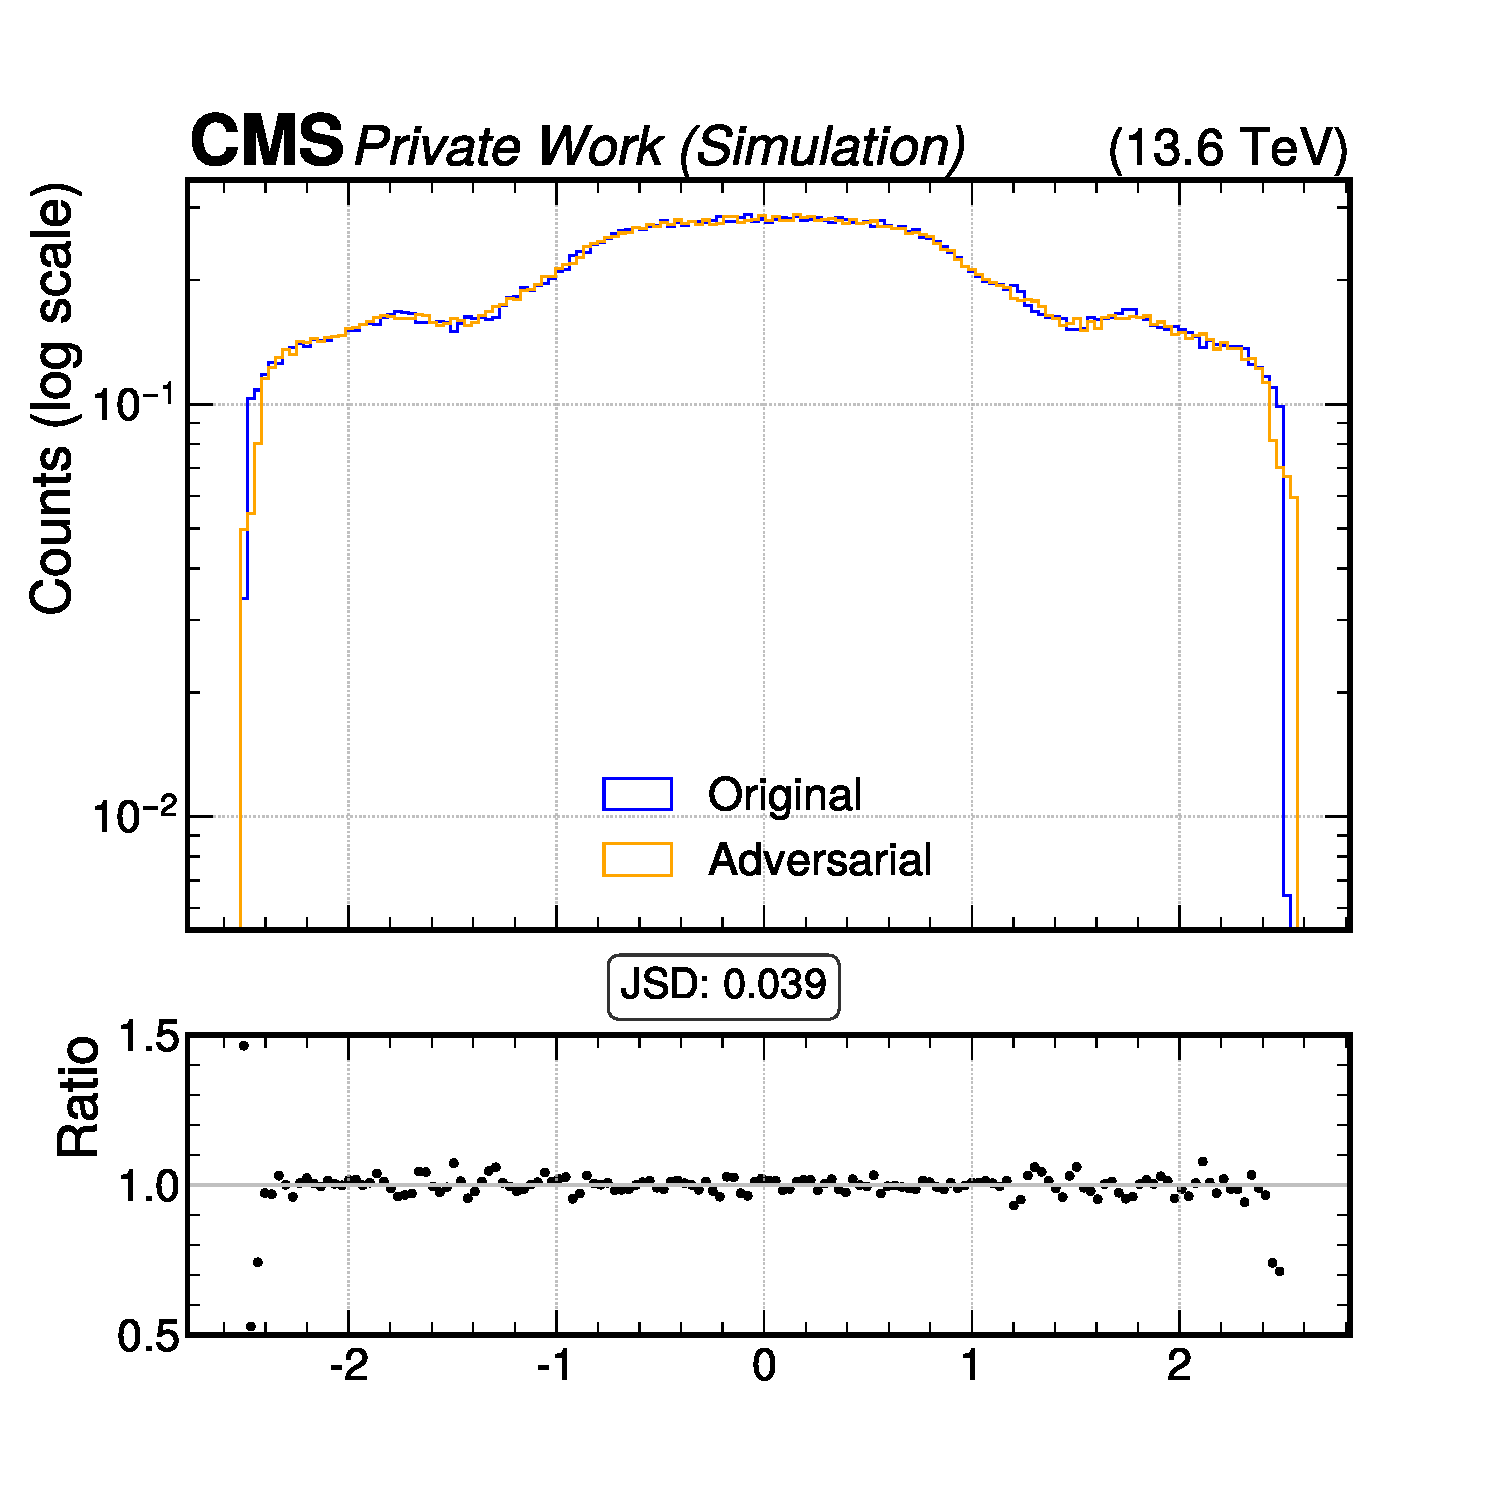
\includegraphics[width=\linewidth]{media/output/features/compare/combined_it_1/cmp_global_features_jet_eta.pdf}
    \caption*{Input similarity for PIP-PGD(1).}
  \end{subfigure}\hfill
  \begin{subfigure}[t]{0.32\textwidth}
    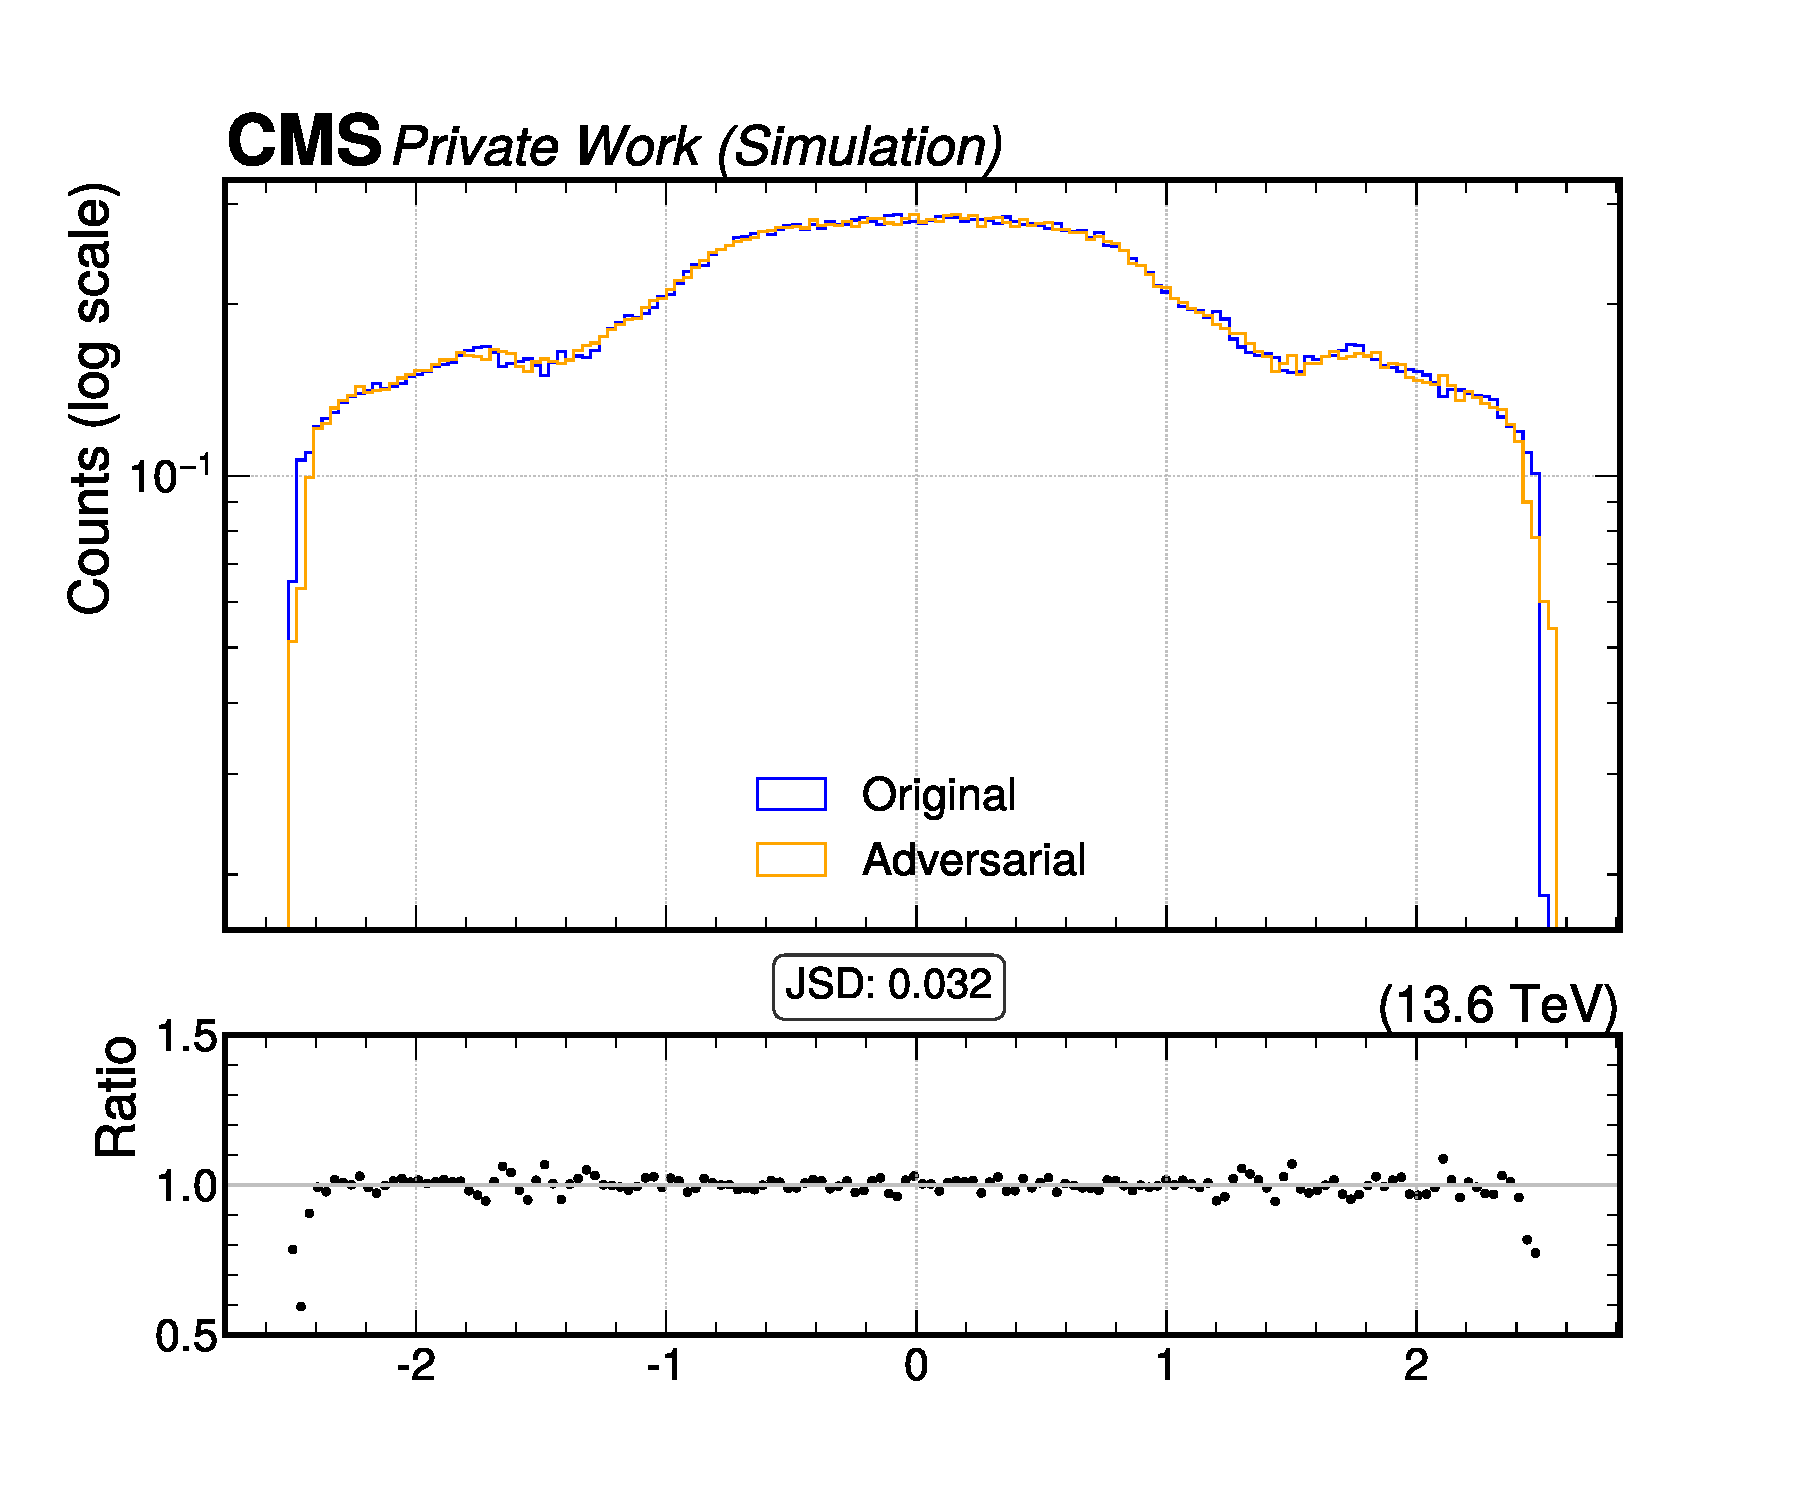
\includegraphics[width=\linewidth]{media/output/features/compare/combined_it_2/cmp_global_features_jet_eta.pdf}
    \caption*{Input similarity for PIP-PGD(2).}
  \end{subfigure}\hfill
  \begin{subfigure}[t]{0.32\textwidth}
    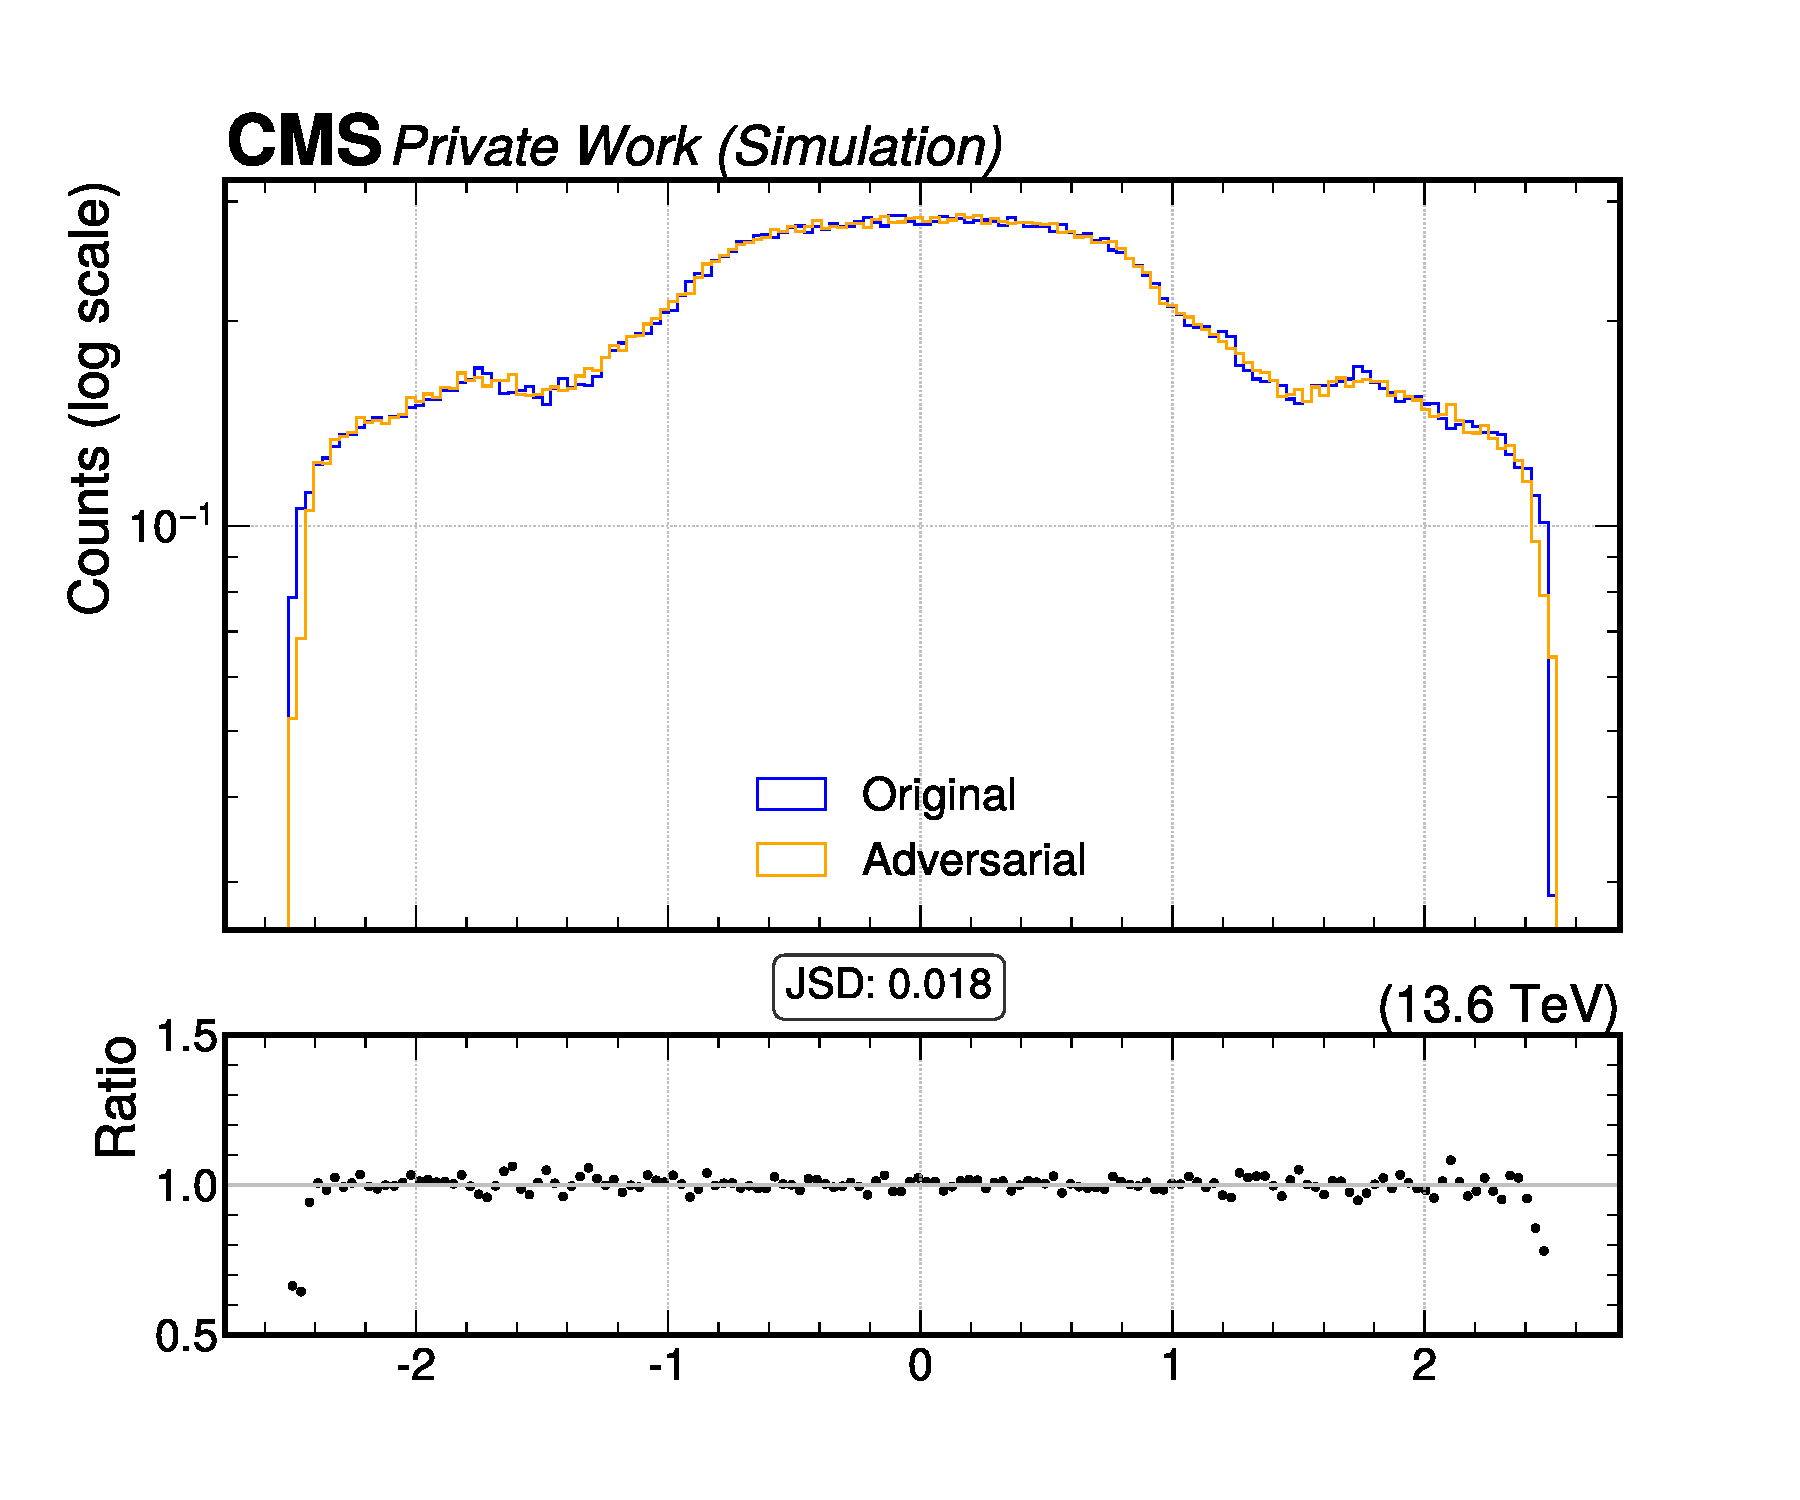
\includegraphics[width=\linewidth]{media/output/features/compare/combined_it_3/cmp_global_features_jet_eta.pdf}
    \caption*{Input similarity for PIP-PGD(3).}
  \end{subfigure}

  \caption*{Histogram of \texttt{jet\_eta} for multiple iterations of PIP-PGD tested against nominal inputs.}
  \label{fig:combined_input_jet_eta}
\end{figure}

\begin{figure}[h]
  \centering
  \begin{subfigure}[t]{0.32\textwidth}
    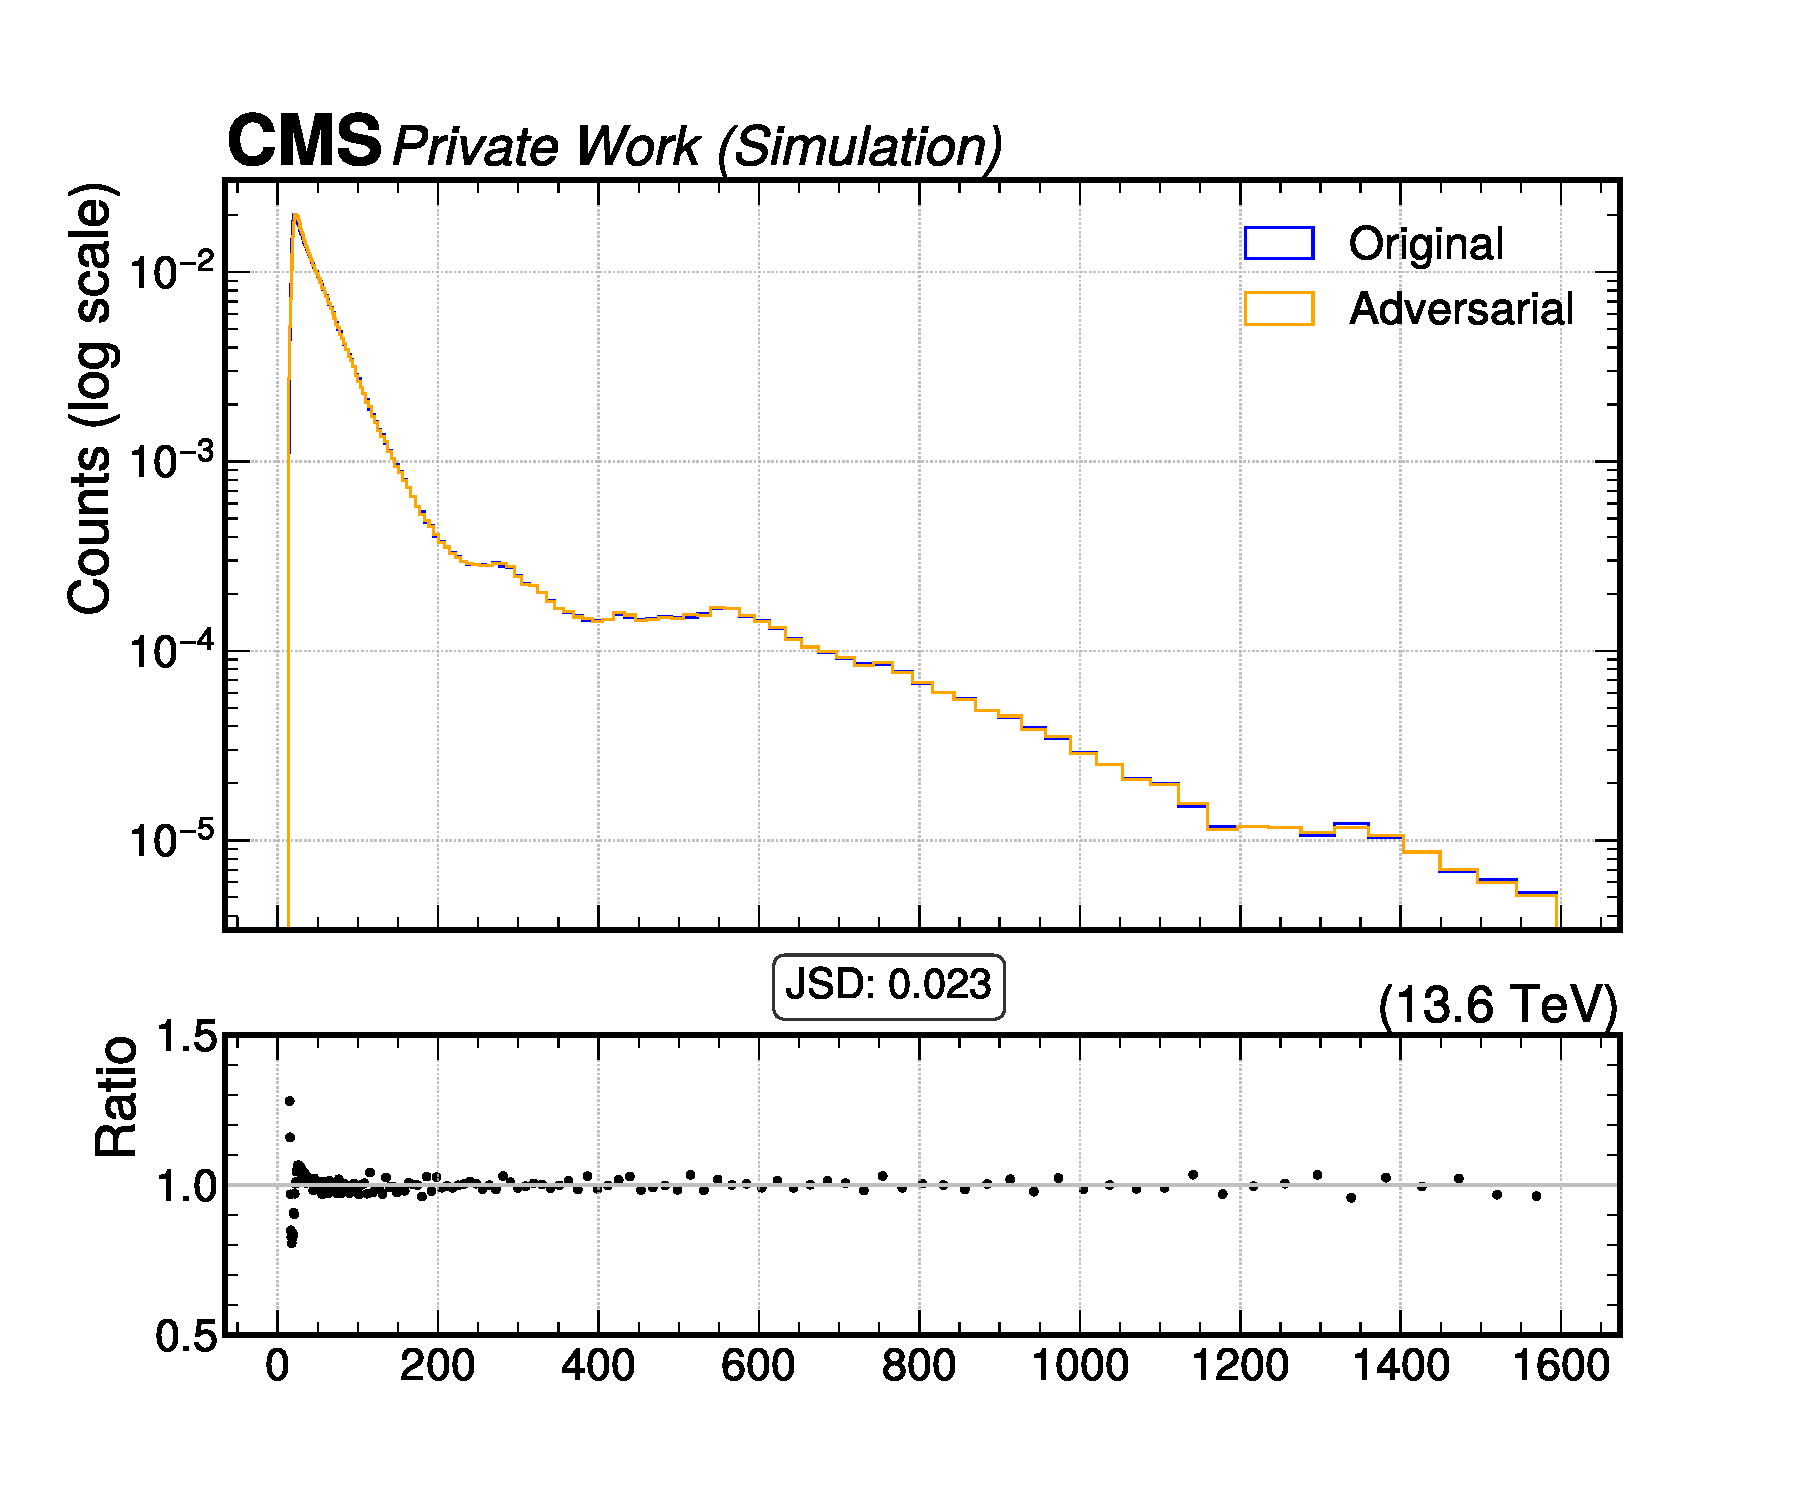
\includegraphics[width=\linewidth]{media/output/features/compare/combined_it_1/cmp_global_features_jet_pt.pdf}
    \caption*{Input similarity for PIP-PGD(1).}
  \end{subfigure}\hfill
  \begin{subfigure}[t]{0.32\textwidth}
    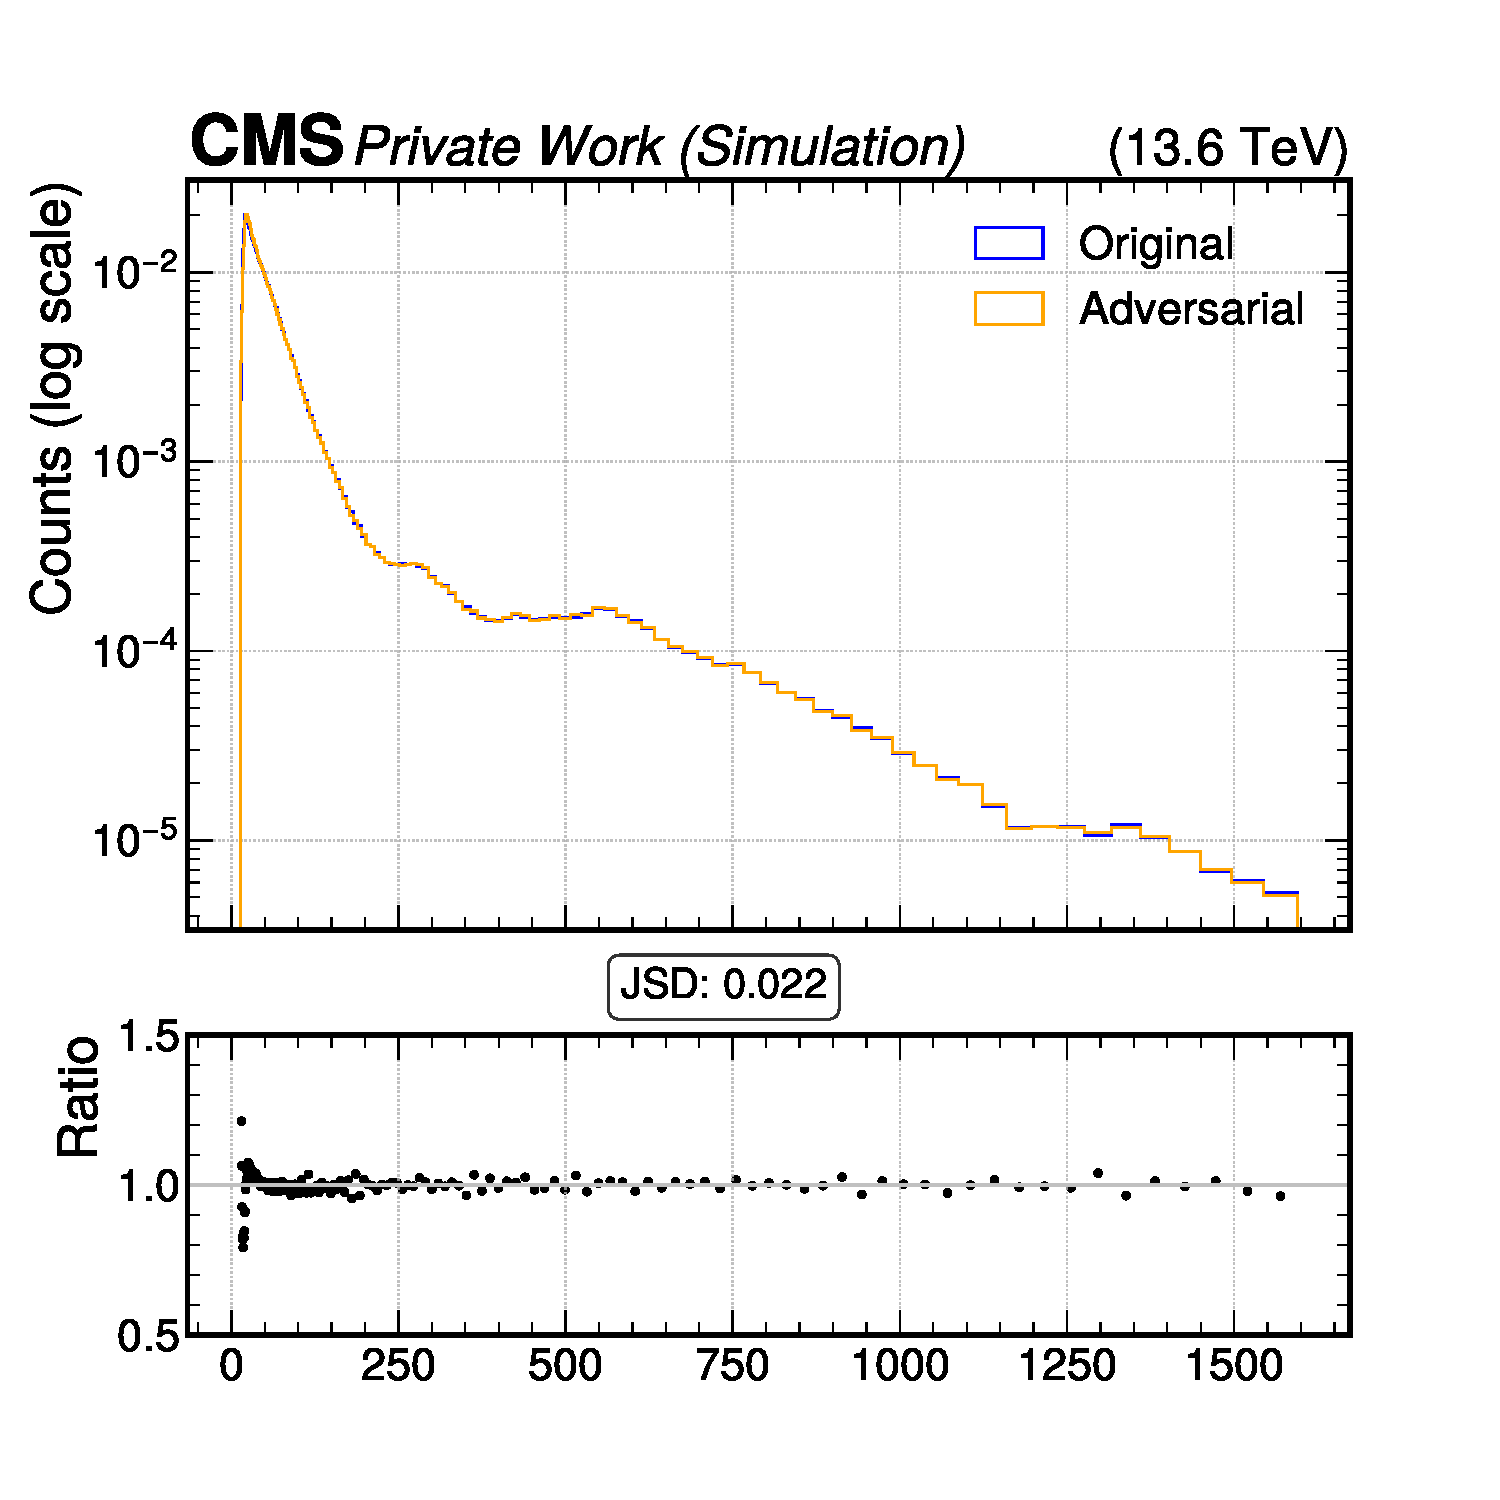
\includegraphics[width=\linewidth]{media/output/features/compare/combined_it_2/cmp_global_features_jet_pt.pdf}
    \caption*{Input similarity for PIP-PGD(2).}
  \end{subfigure}\hfill
  \begin{subfigure}[t]{0.32\textwidth}
    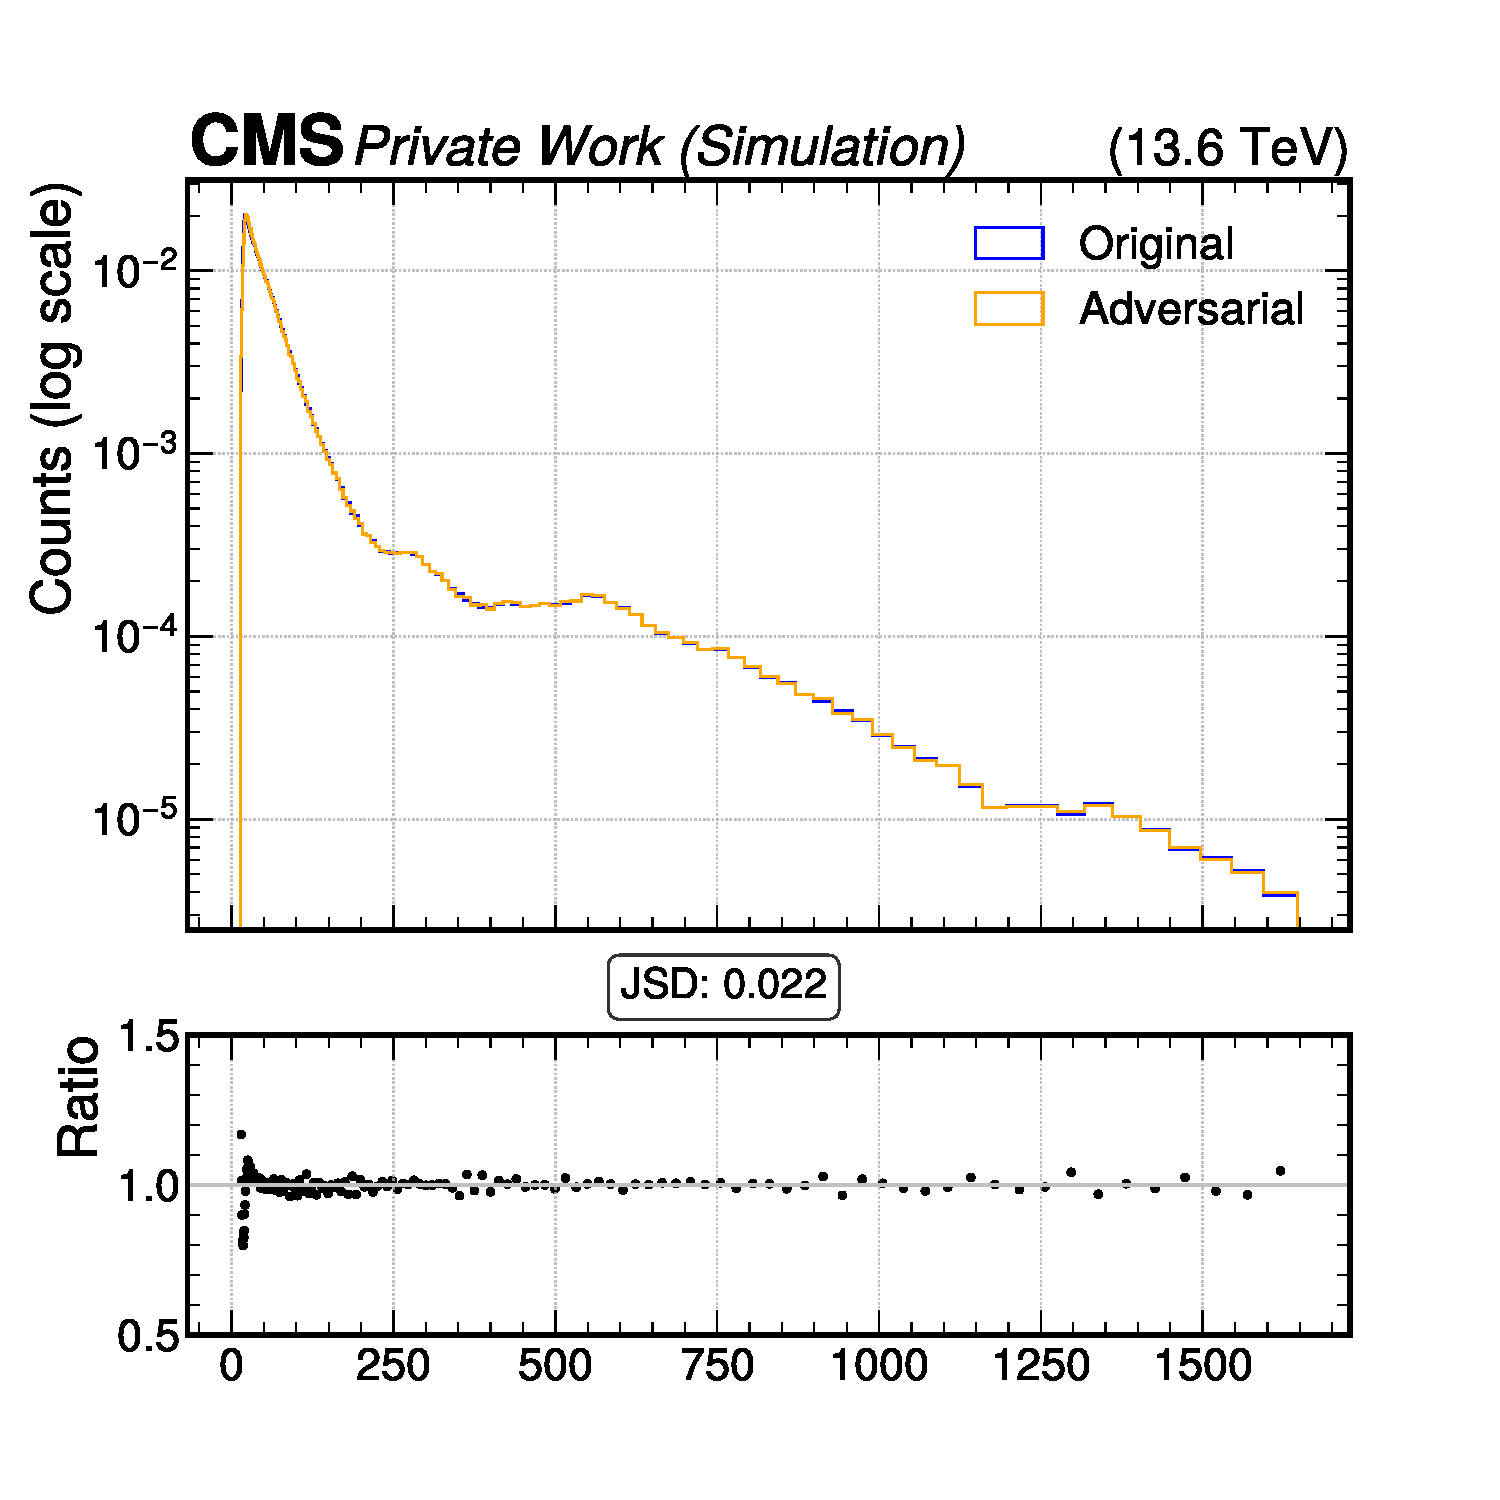
\includegraphics[width=\linewidth]{media/output/features/compare/combined_it_3/cmp_global_features_jet_pt.pdf}
    \caption*{Input similarity for PIP-PGD(3).}
  \end{subfigure}

  \caption*{Histogram of \texttt{jet\_pt} for multiple iterations of PIP-PGD tested against nominal inputs.}
  \label{fig:combined_input_jet_pt}
\end{figure}

\begin{figure}[h]
  \centering
  \begin{subfigure}[t]{0.32\textwidth}
    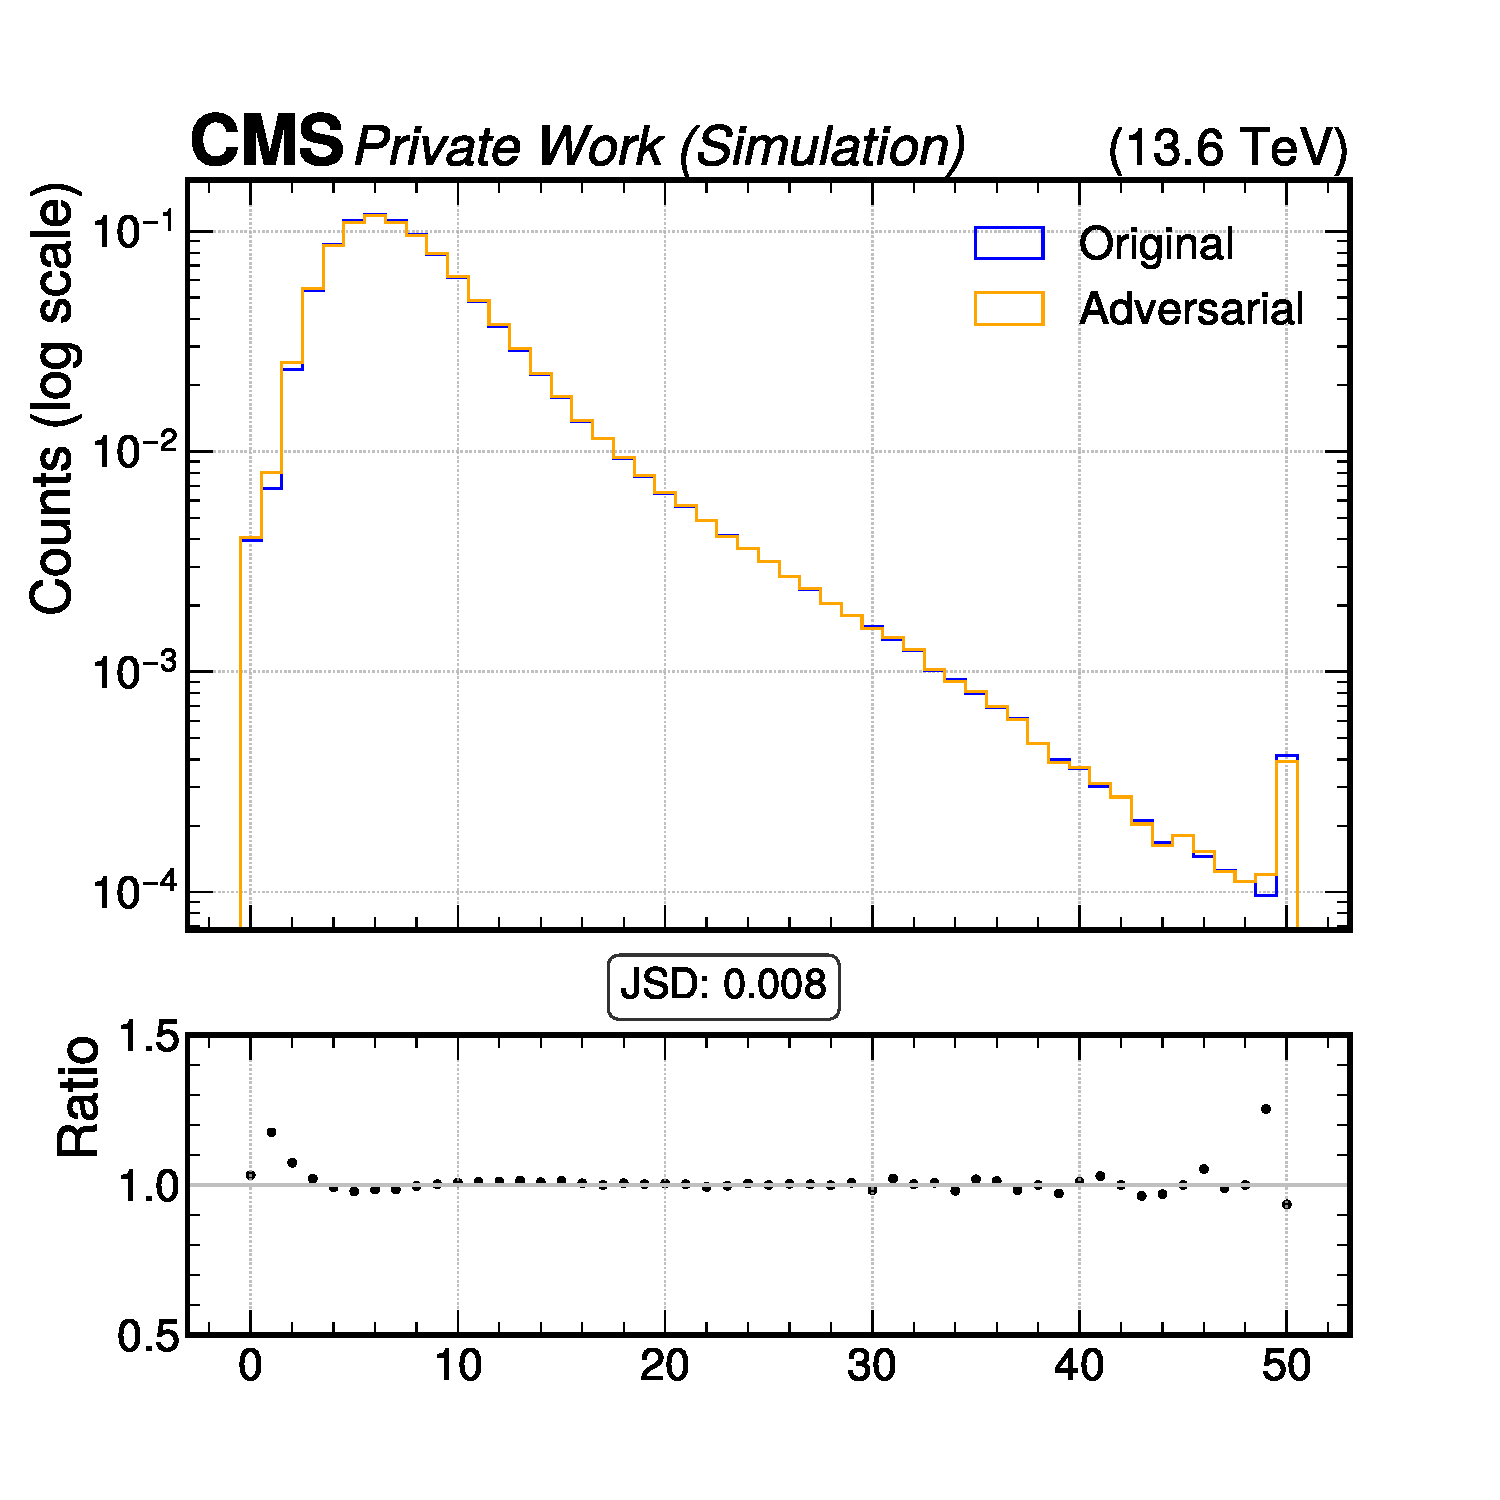
\includegraphics[width=\linewidth]{media/output/features/compare/combined_it_1/cmp_global_features_n_Cpfcand.pdf}
    \caption*{Input similarity for PIP-PGD(1).}
  \end{subfigure}\hfill
  \begin{subfigure}[t]{0.32\textwidth}
    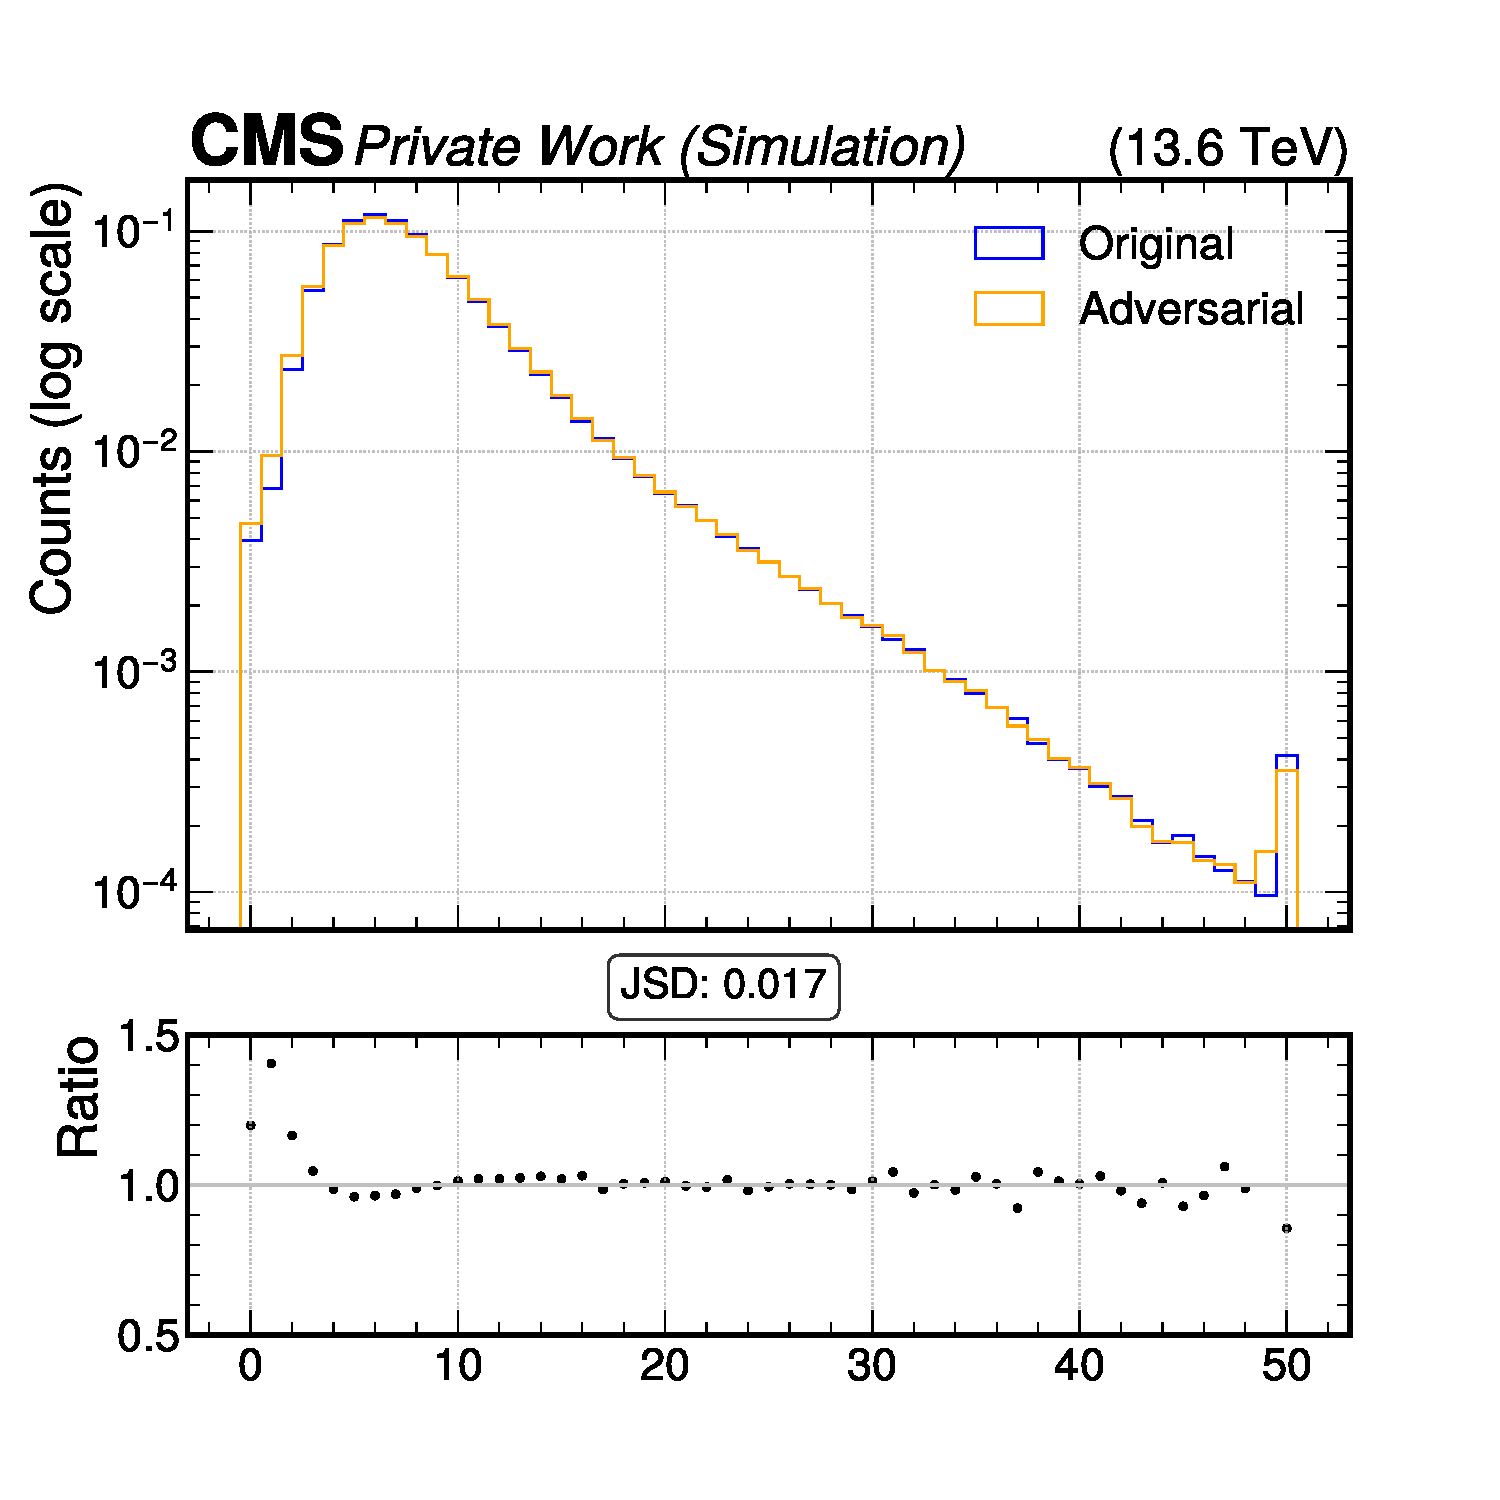
\includegraphics[width=\linewidth]{media/output/features/compare/combined_it_2/cmp_global_features_n_Cpfcand.pdf}
    \caption*{Input similarity for PIP-PGD(2).}
  \end{subfigure}\hfill
  \begin{subfigure}[t]{0.32\textwidth}
    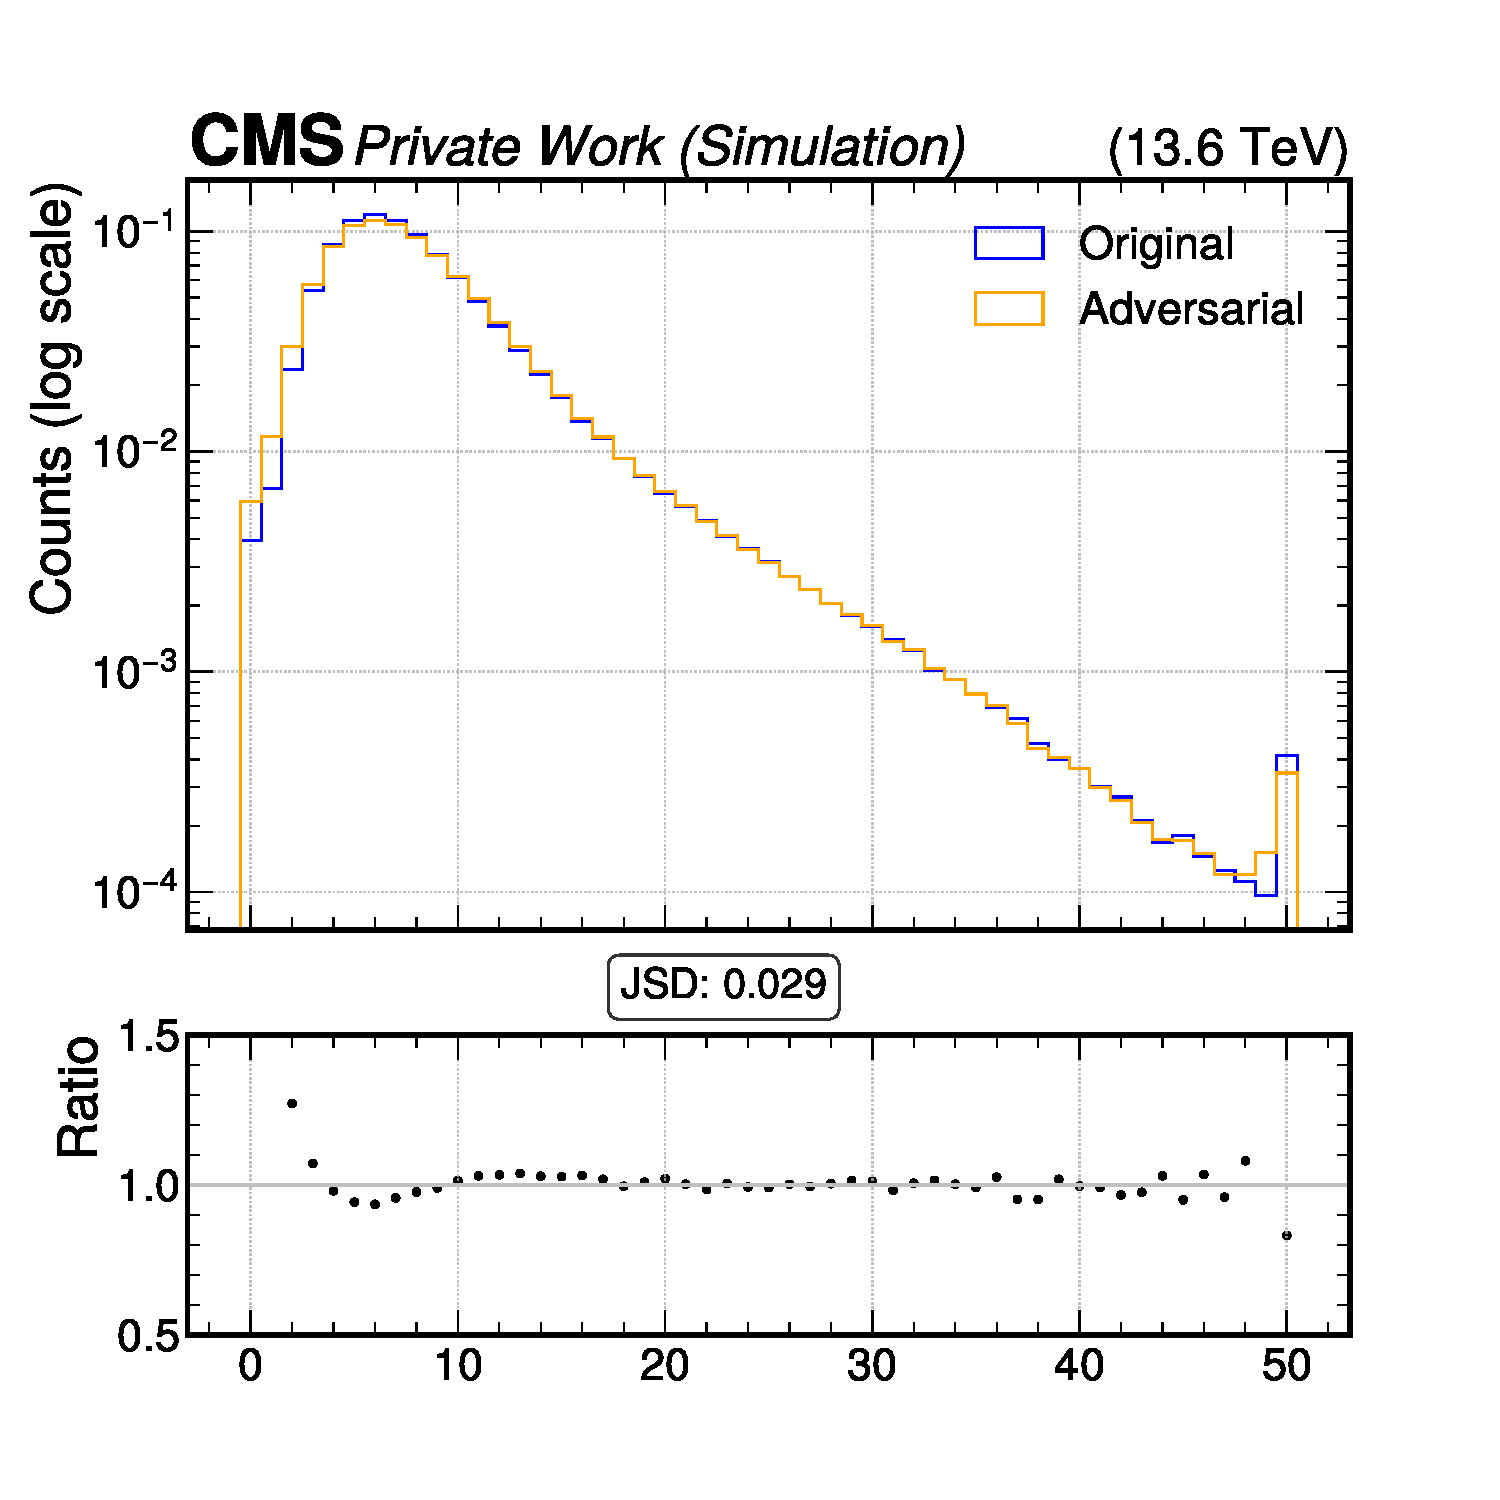
\includegraphics[width=\linewidth]{media/output/features/compare/combined_it_3/cmp_global_features_n_Cpfcand.pdf}
    \caption*{Input similarity for PIP-PGD(3).}
  \end{subfigure}

  \caption*{Histogram of \texttt{n\_Cpfcand} for multiple iterations of PIP-PGD tested against nominal inputs.}
  \label{fig:combined_input_n_Cpfcand}
\end{figure}

\begin{figure}[h]
  \centering
  \begin{subfigure}[t]{0.32\textwidth}
    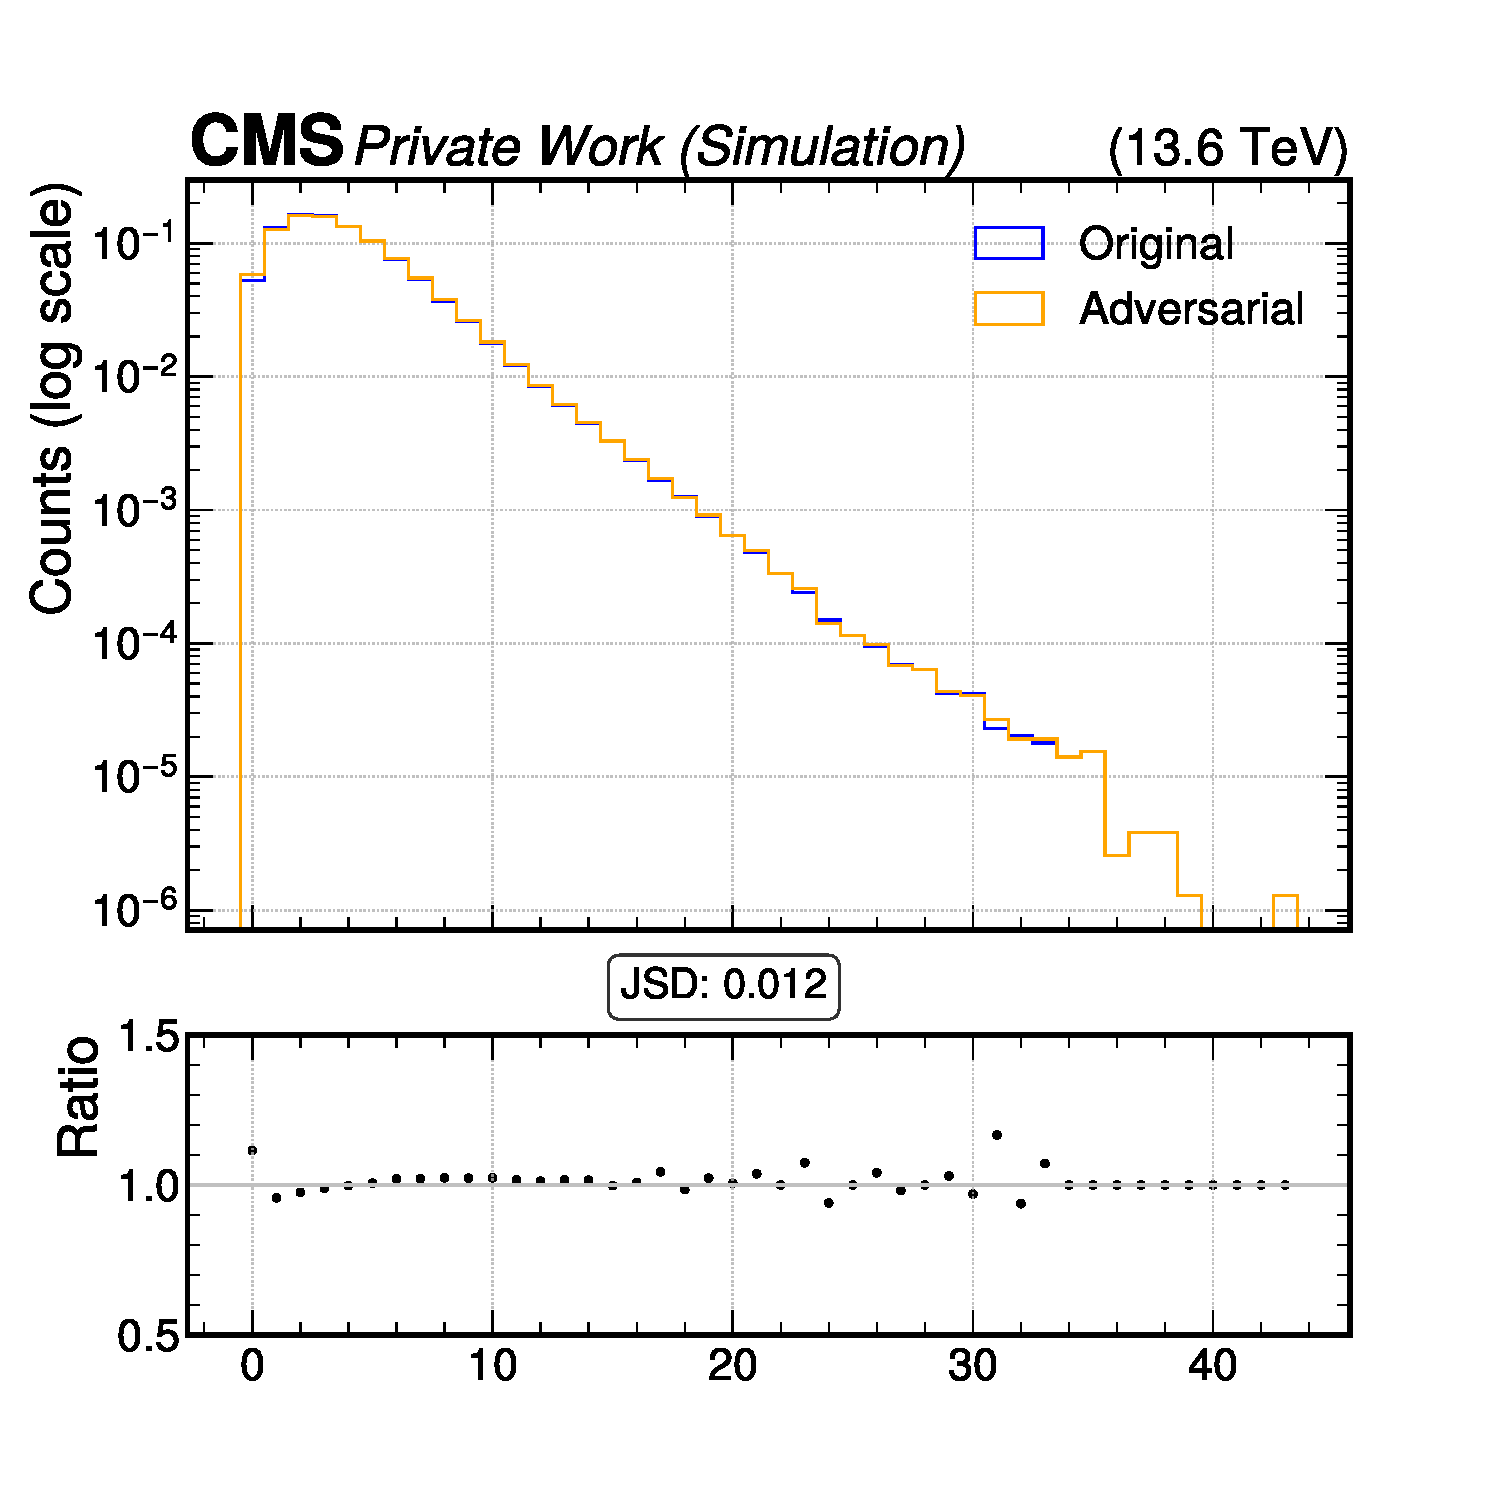
\includegraphics[width=\linewidth]{media/output/features/compare/combined_it_1/cmp_global_features_n_Npfcand.pdf}
    \caption*{Input similarity for PIP-PGD(1).}
  \end{subfigure}\hfill
  \begin{subfigure}[t]{0.32\textwidth}
    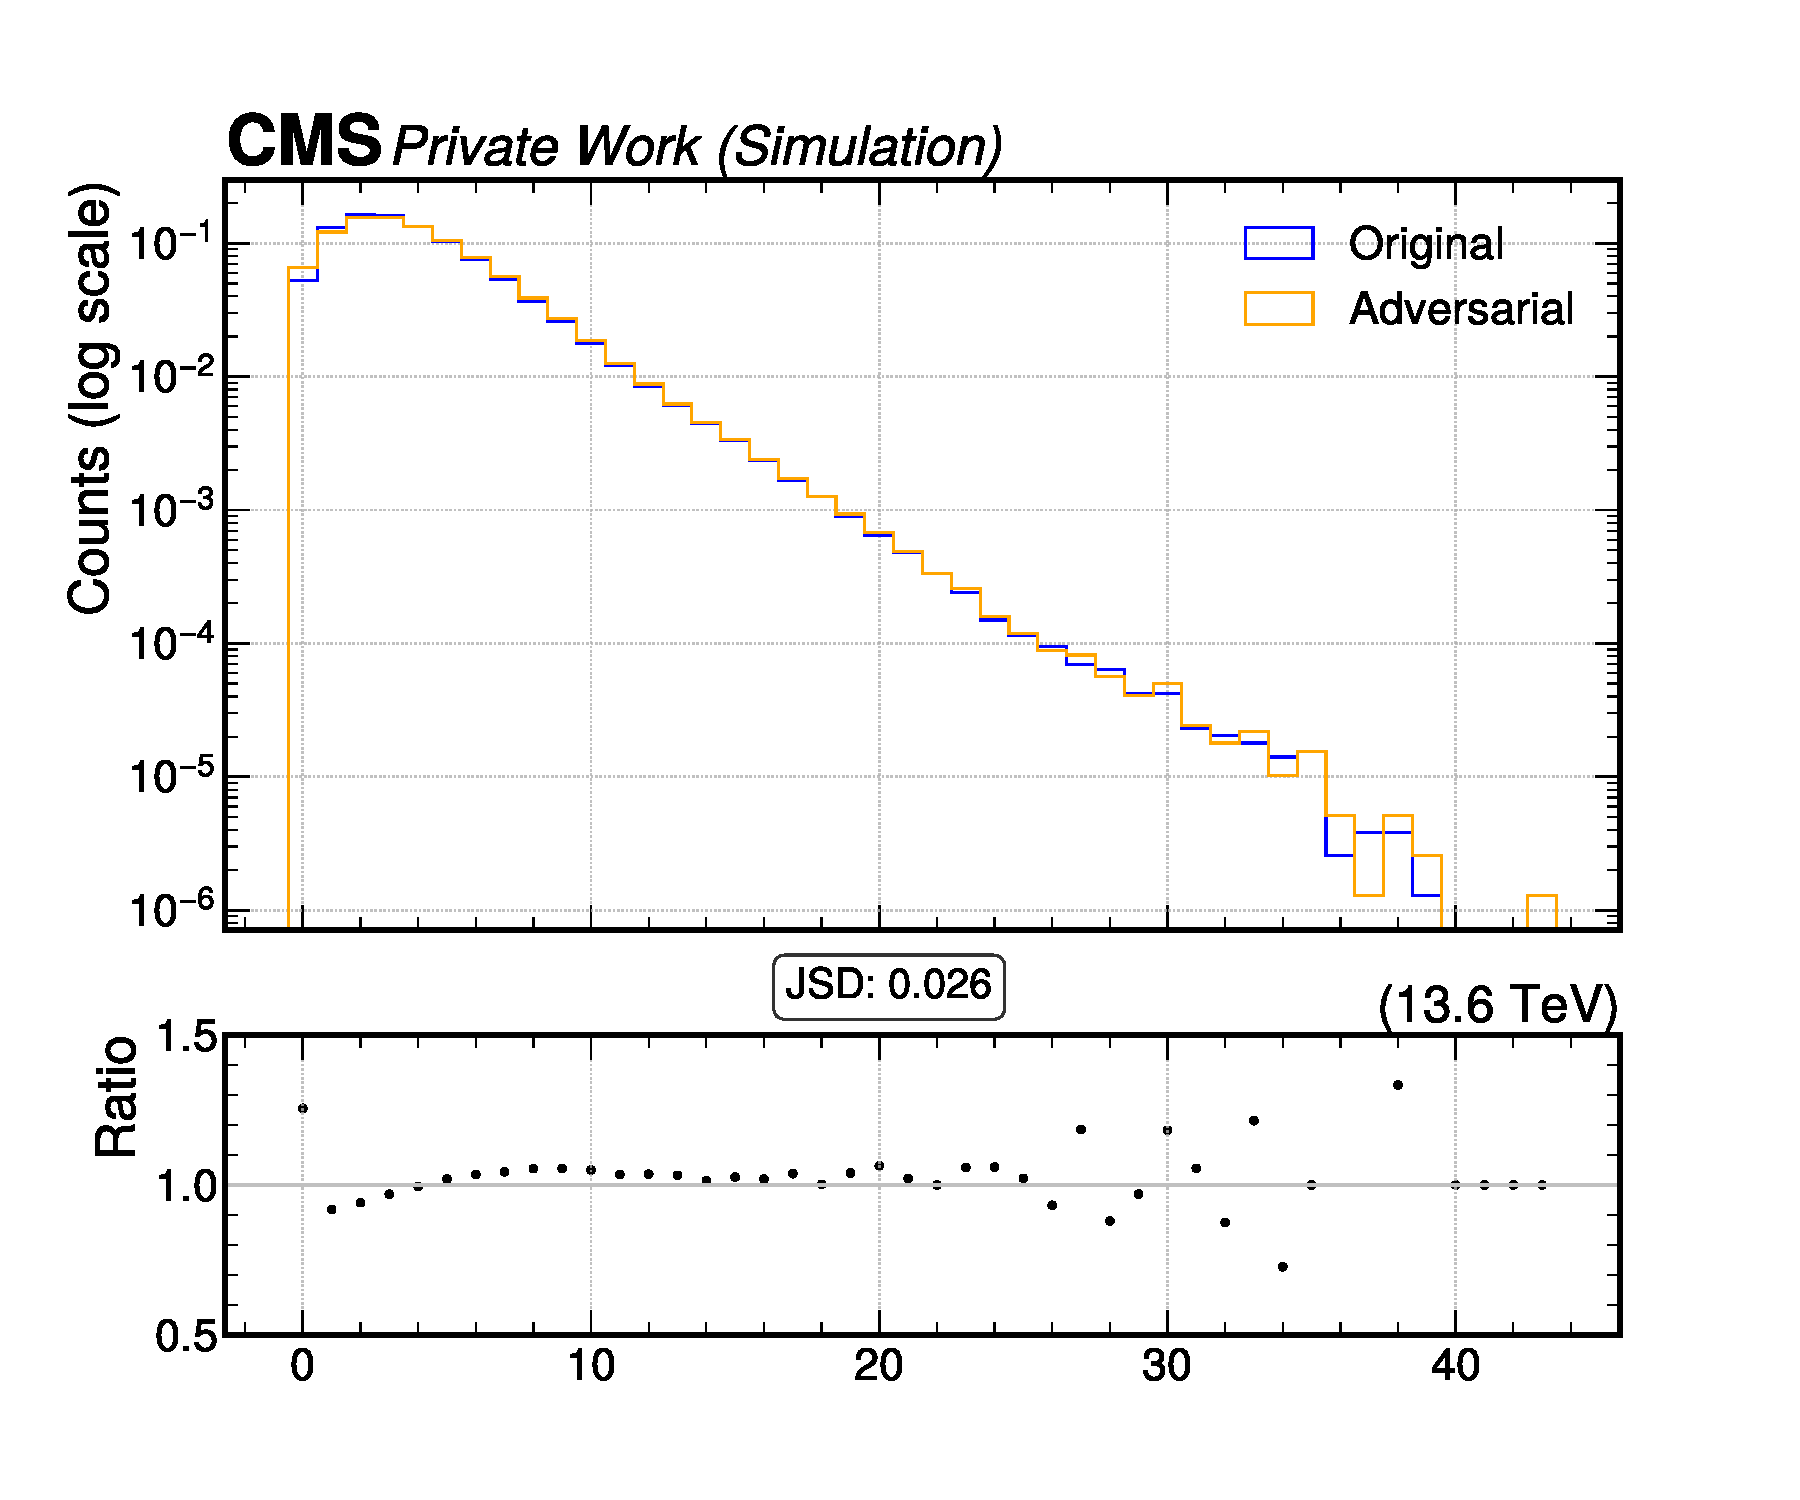
\includegraphics[width=\linewidth]{media/output/features/compare/combined_it_2/cmp_global_features_n_Npfcand.pdf}
    \caption*{Input similarity for PIP-PGD(2).}
  \end{subfigure}\hfill
  \begin{subfigure}[t]{0.32\textwidth}
    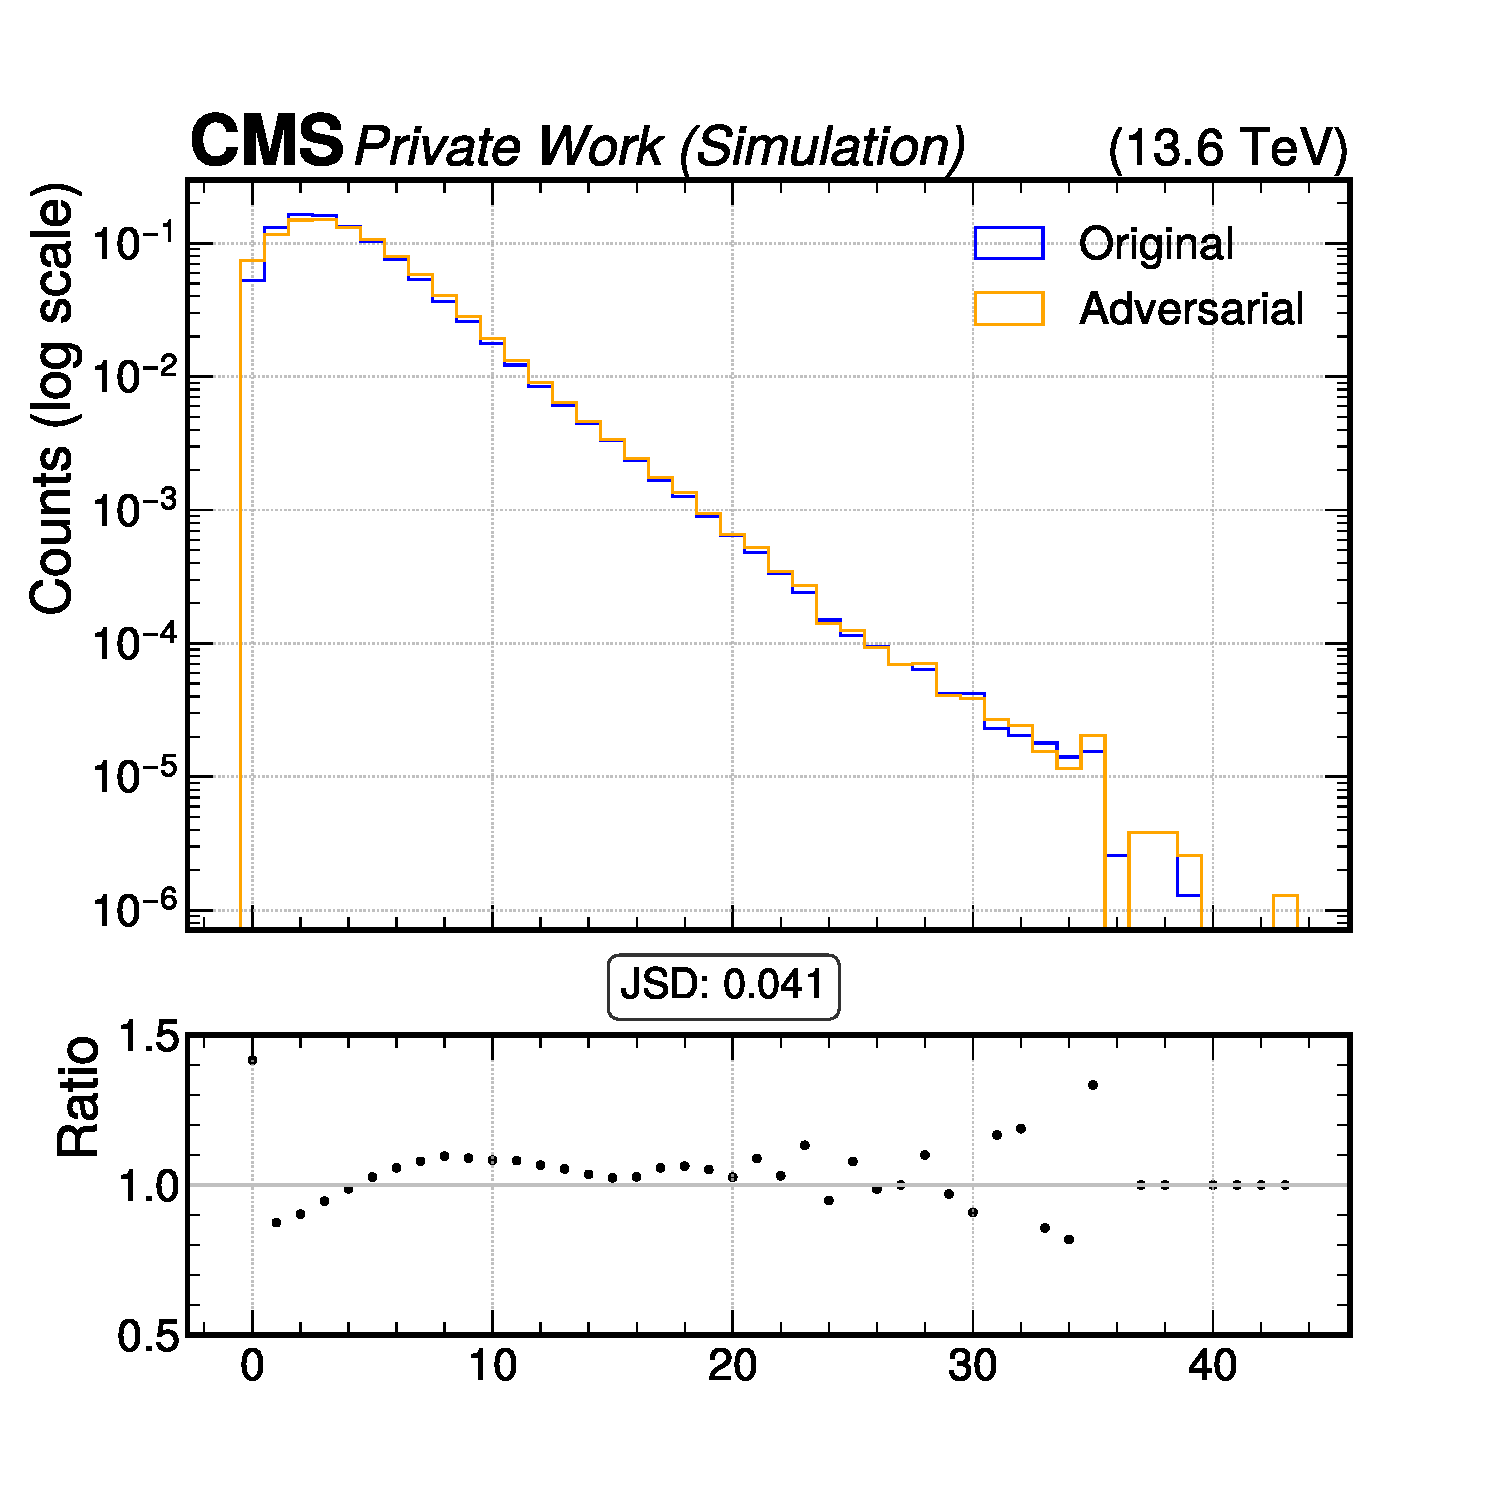
\includegraphics[width=\linewidth]{media/output/features/compare/combined_it_3/cmp_global_features_n_Npfcand.pdf}
    \caption*{Input similarity for PIP-PGD(3).}
  \end{subfigure}

  \caption*{Histogram of \texttt{n\_Npfcand} for multiple iterations of PIP-PGD tested against nominal inputs.}
  \label{fig:combined_input_n_Npfcand}
\end{figure}

\begin{figure}[h]
  \centering
  \begin{subfigure}[t]{0.32\textwidth}
    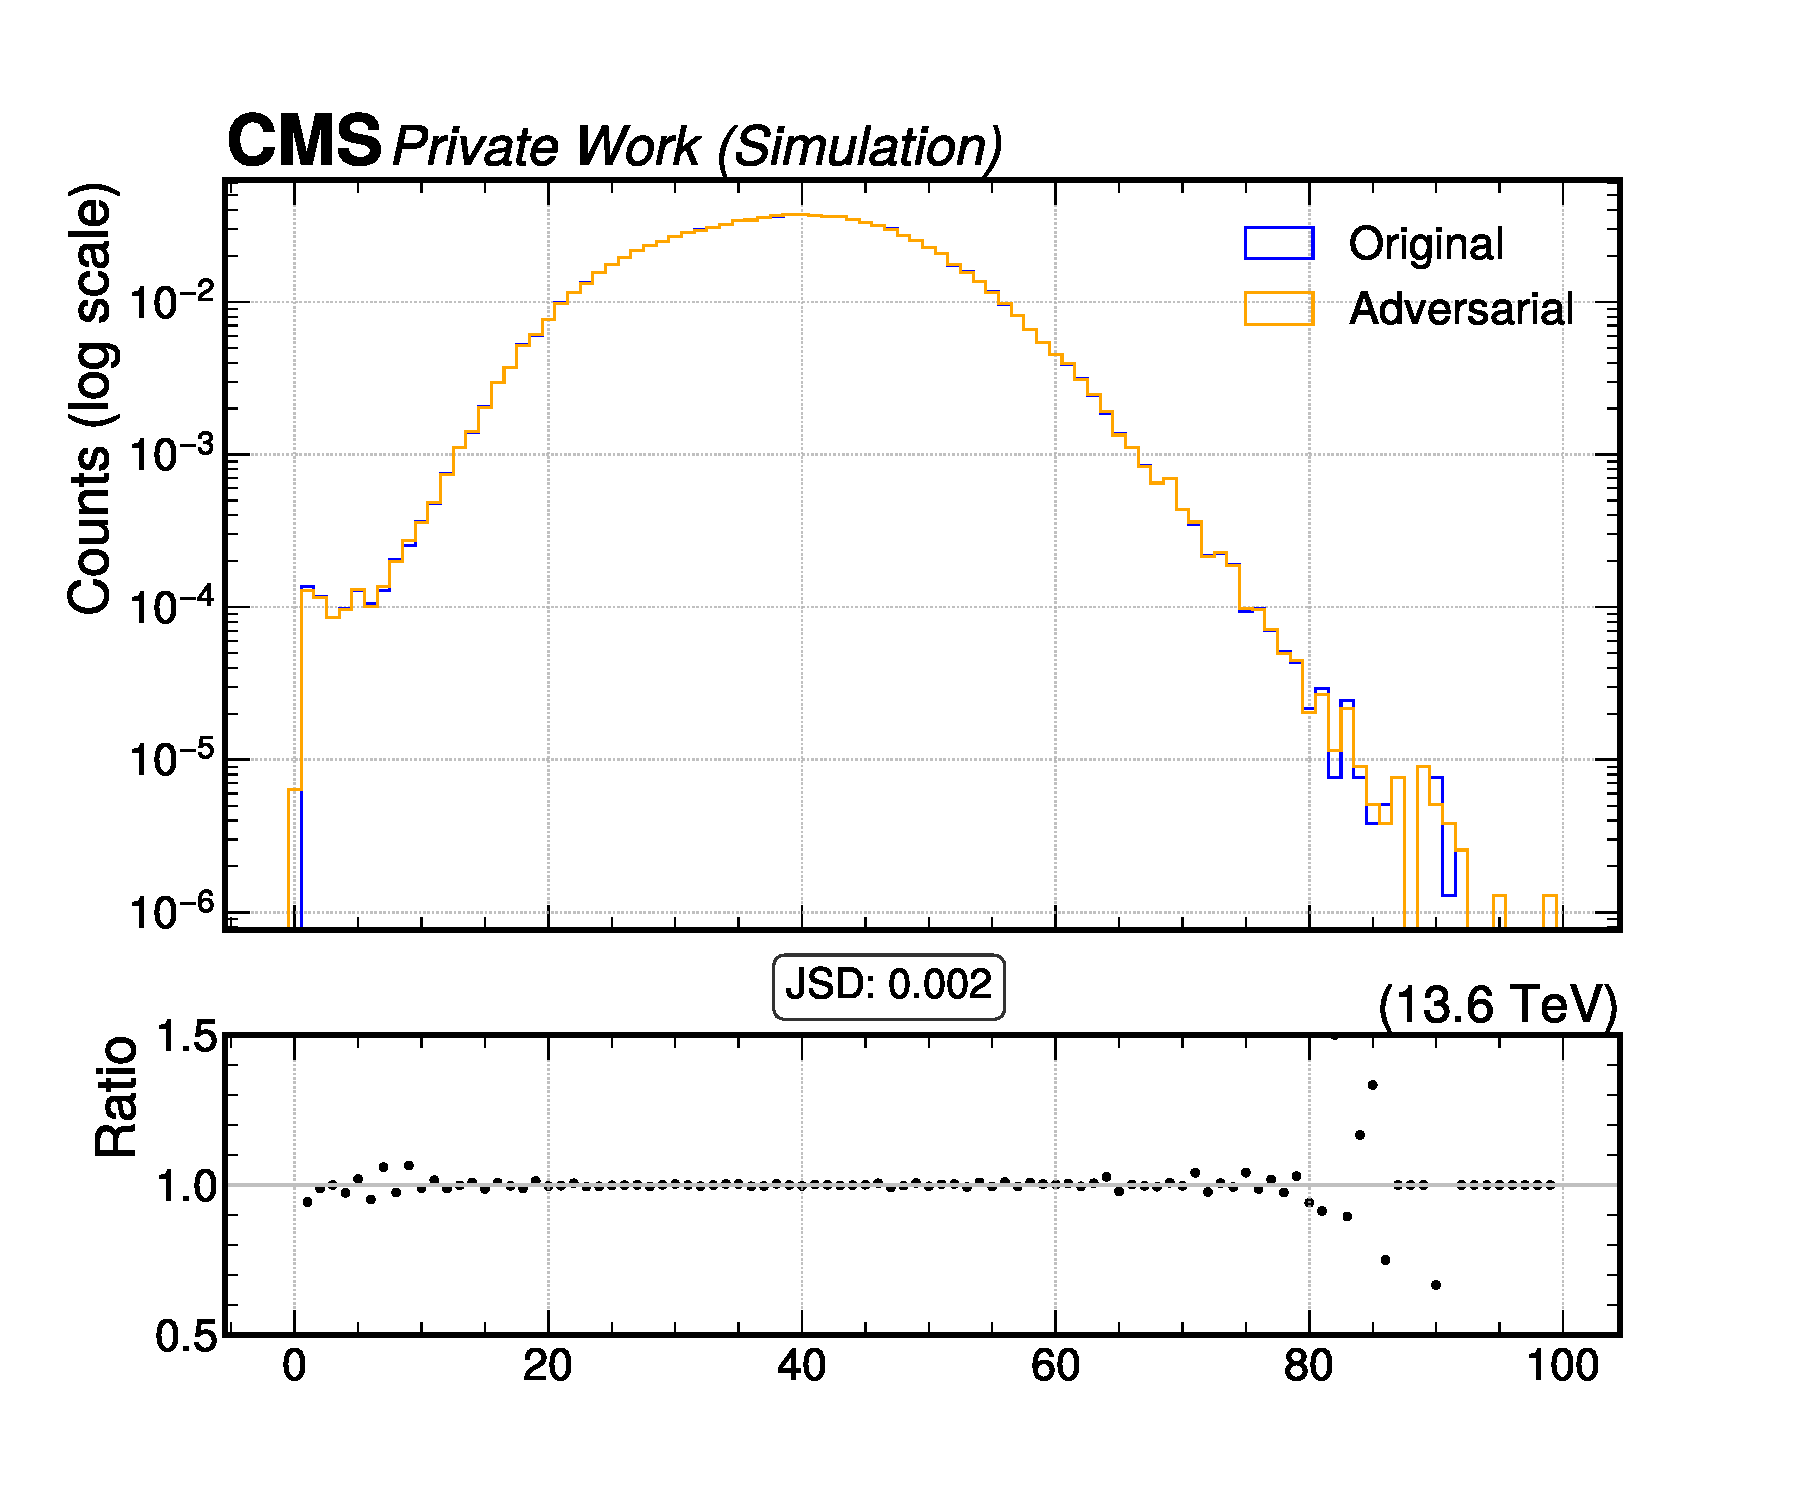
\includegraphics[width=\linewidth]{media/output/features/compare/combined_it_1/cmp_global_features_npv.pdf}
    \caption*{Input similarity for PIP-PGD(1).}
  \end{subfigure}\hfill
  \begin{subfigure}[t]{0.32\textwidth}
    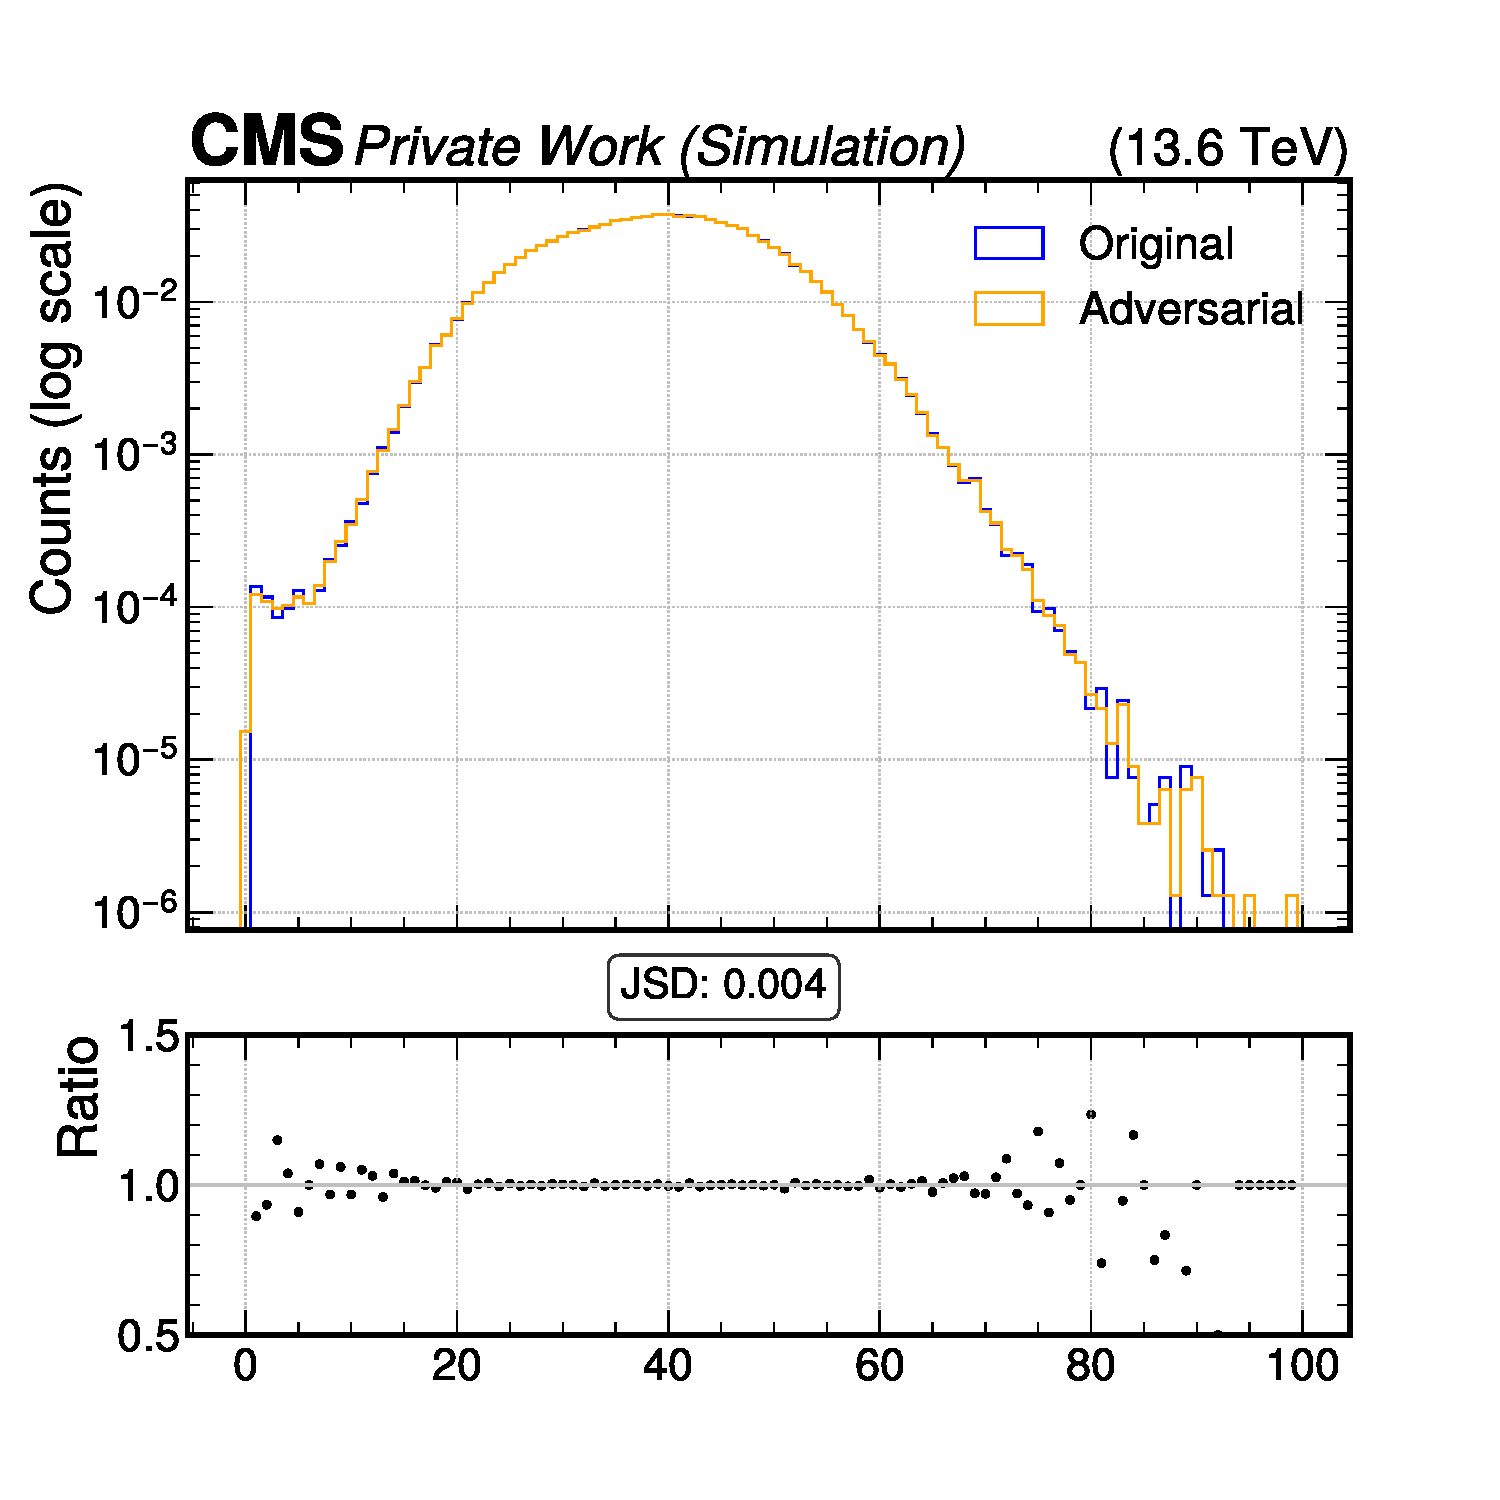
\includegraphics[width=\linewidth]{media/output/features/compare/combined_it_2/cmp_global_features_npv.pdf}
    \caption*{Input similarity for PIP-PGD(2).}
  \end{subfigure}\hfill
  \begin{subfigure}[t]{0.32\textwidth}
    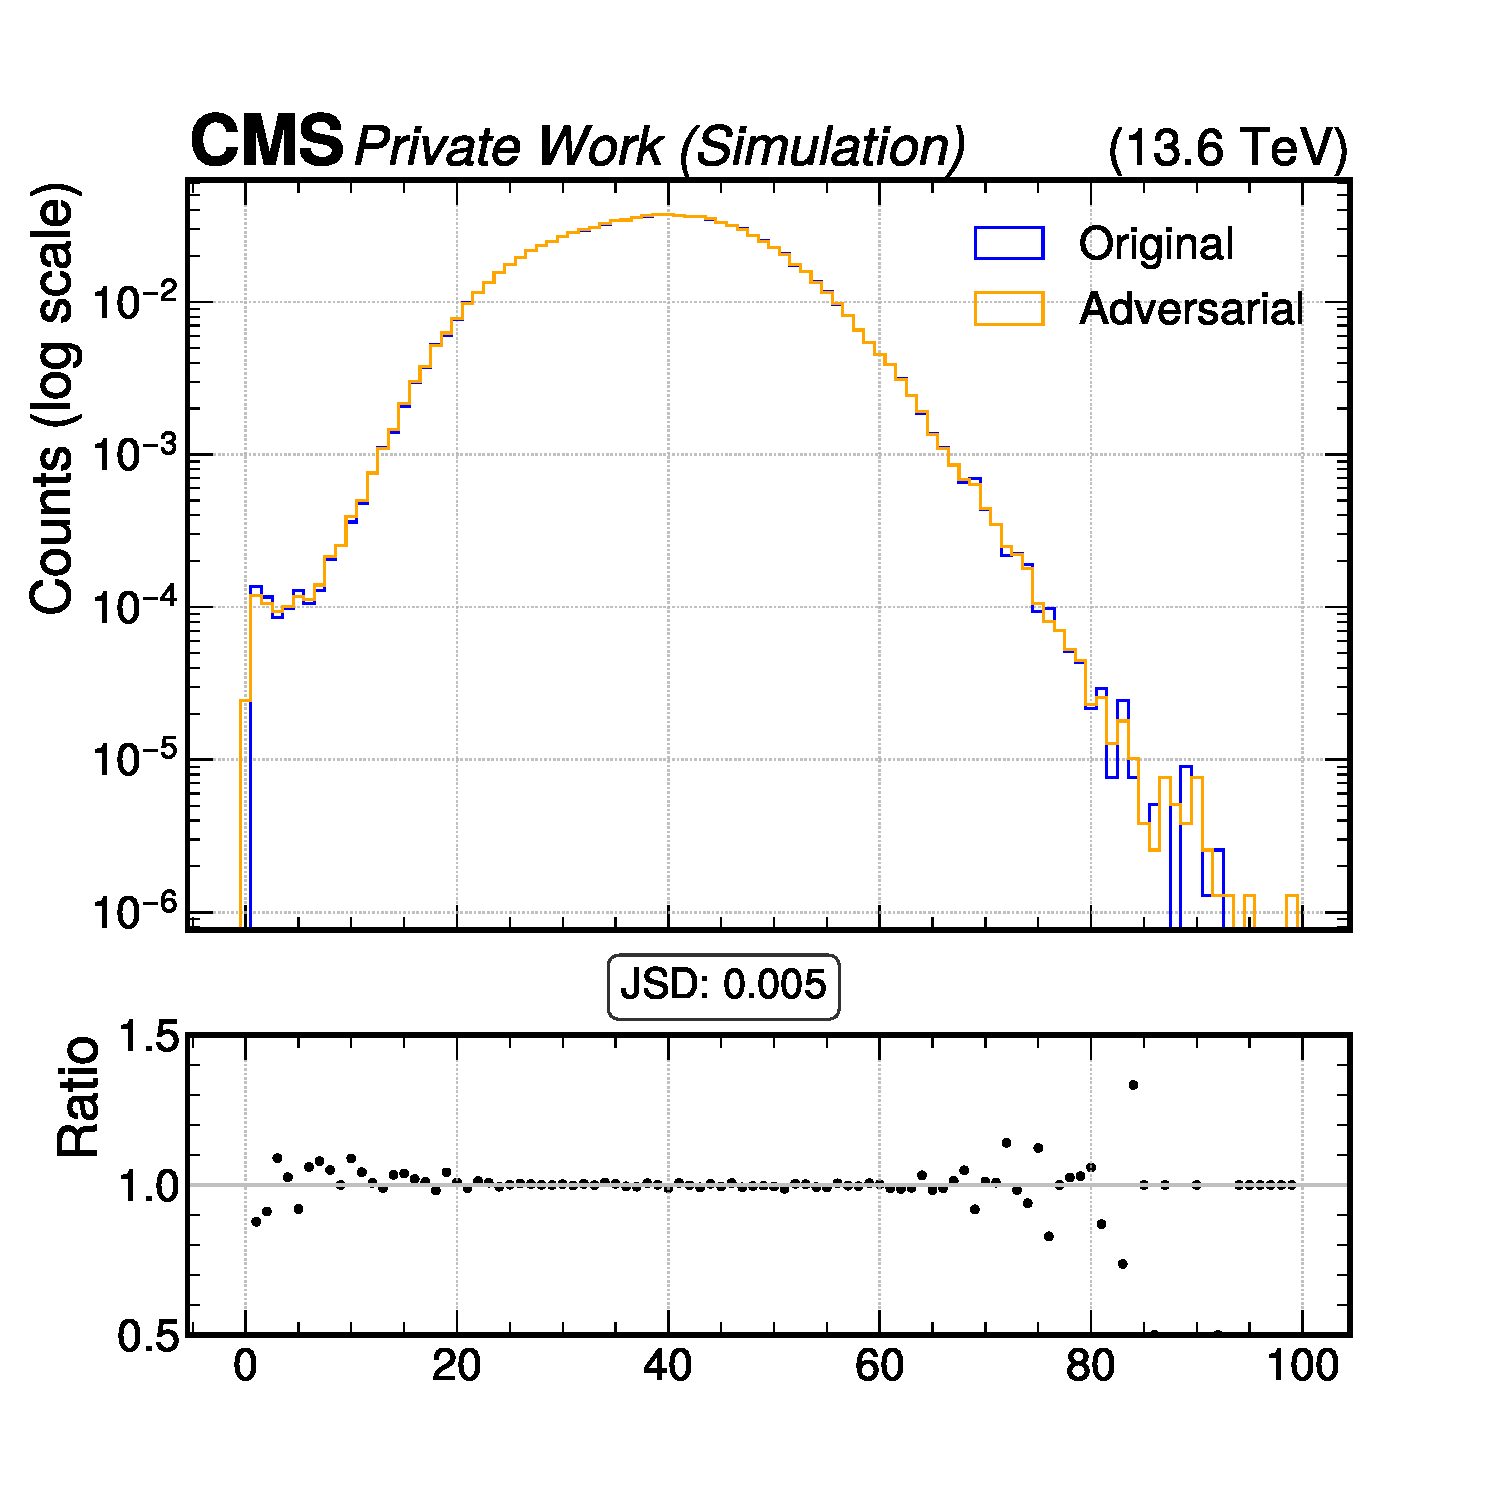
\includegraphics[width=\linewidth]{media/output/features/compare/combined_it_3/cmp_global_features_npv.pdf}
    \caption*{Input similarity for PIP-PGD(3).}
  \end{subfigure}

  \caption*{Histogram of \texttt{npv} for multiple iterations of PIP-PGD tested against nominal inputs.}
  \label{fig:combined_input_npv}
\end{figure}

\begin{figure}[h]
  \centering
  \begin{subfigure}[t]{0.32\textwidth}
    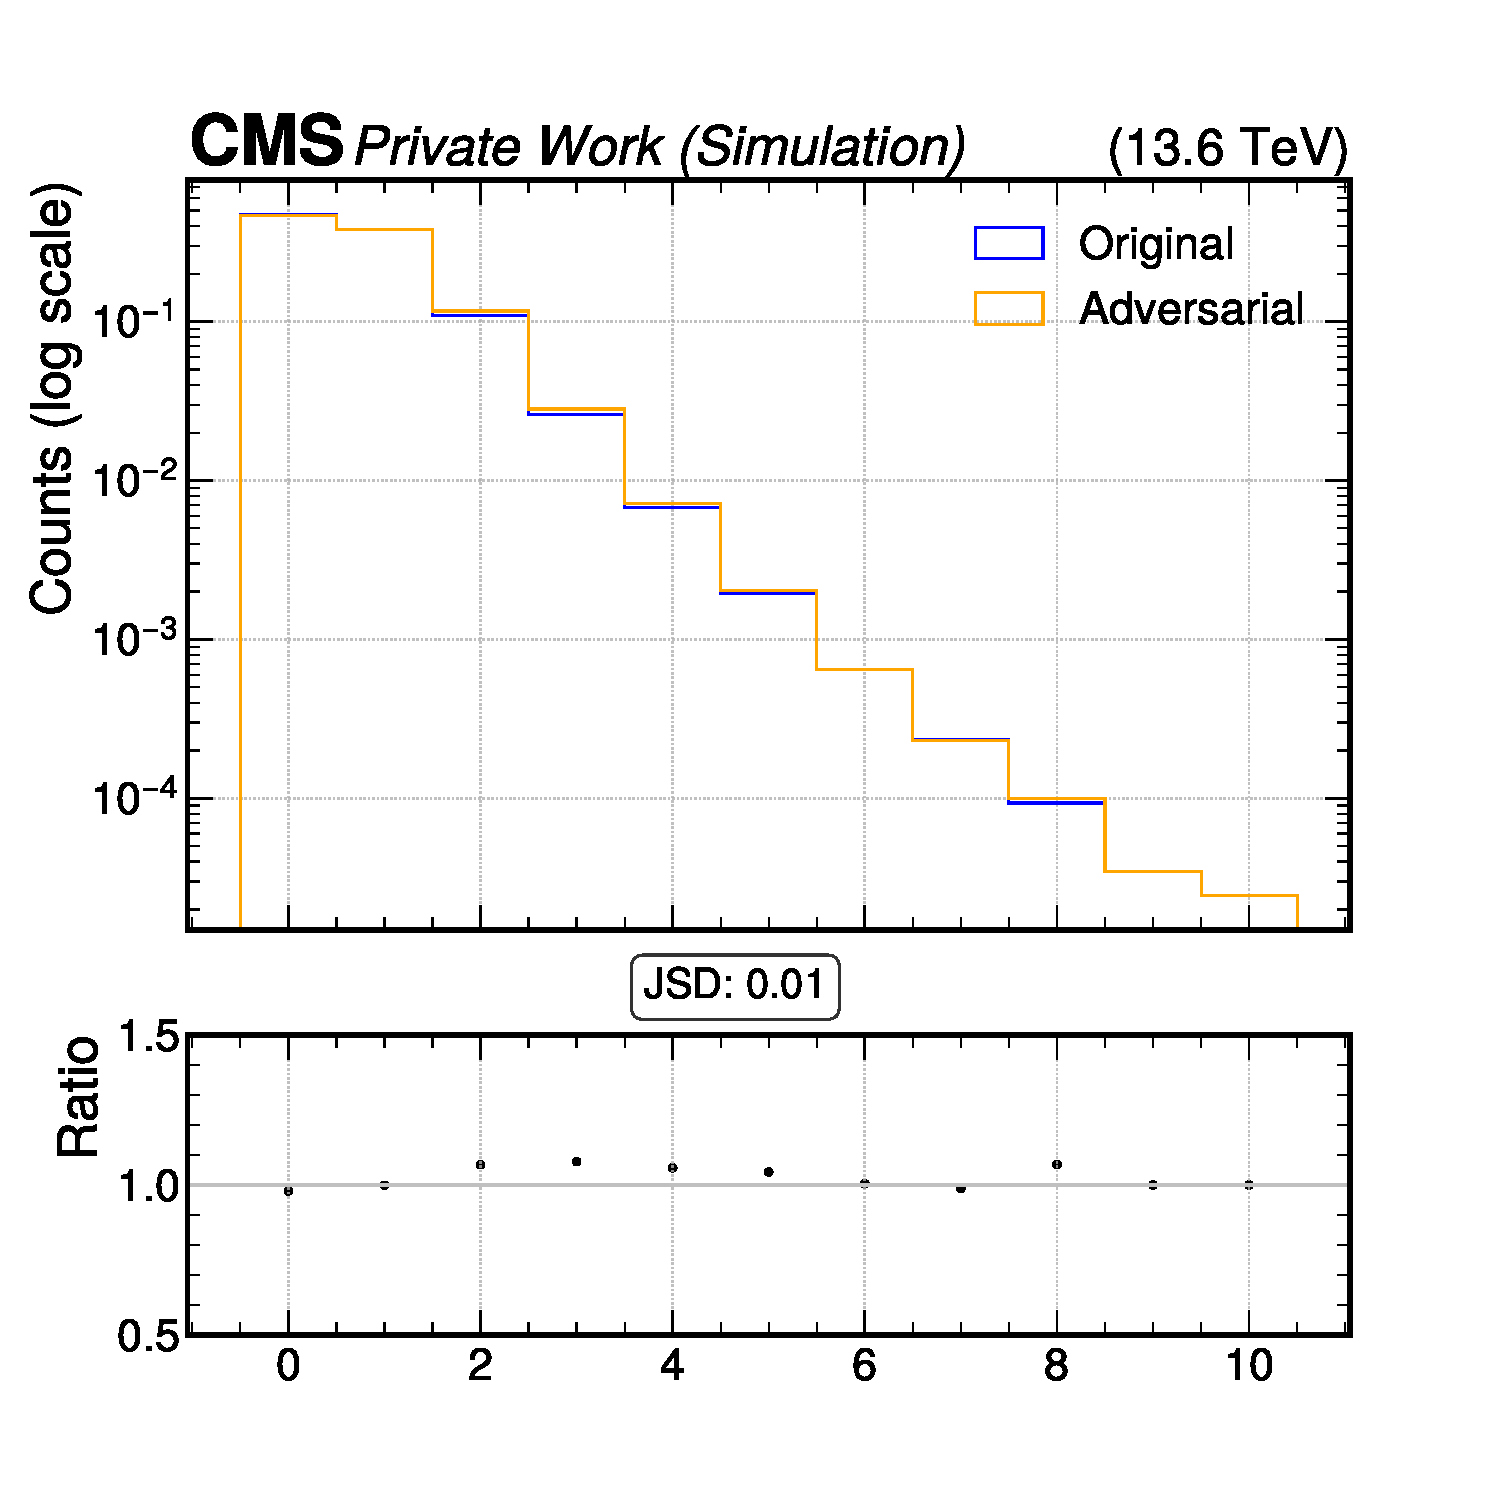
\includegraphics[width=\linewidth]{media/output/features/compare/combined_it_1/cmp_global_features_nsv.pdf}
    \caption*{Input similarity for PIP-PGD(1).}
  \end{subfigure}\hfill
  \begin{subfigure}[t]{0.32\textwidth}
    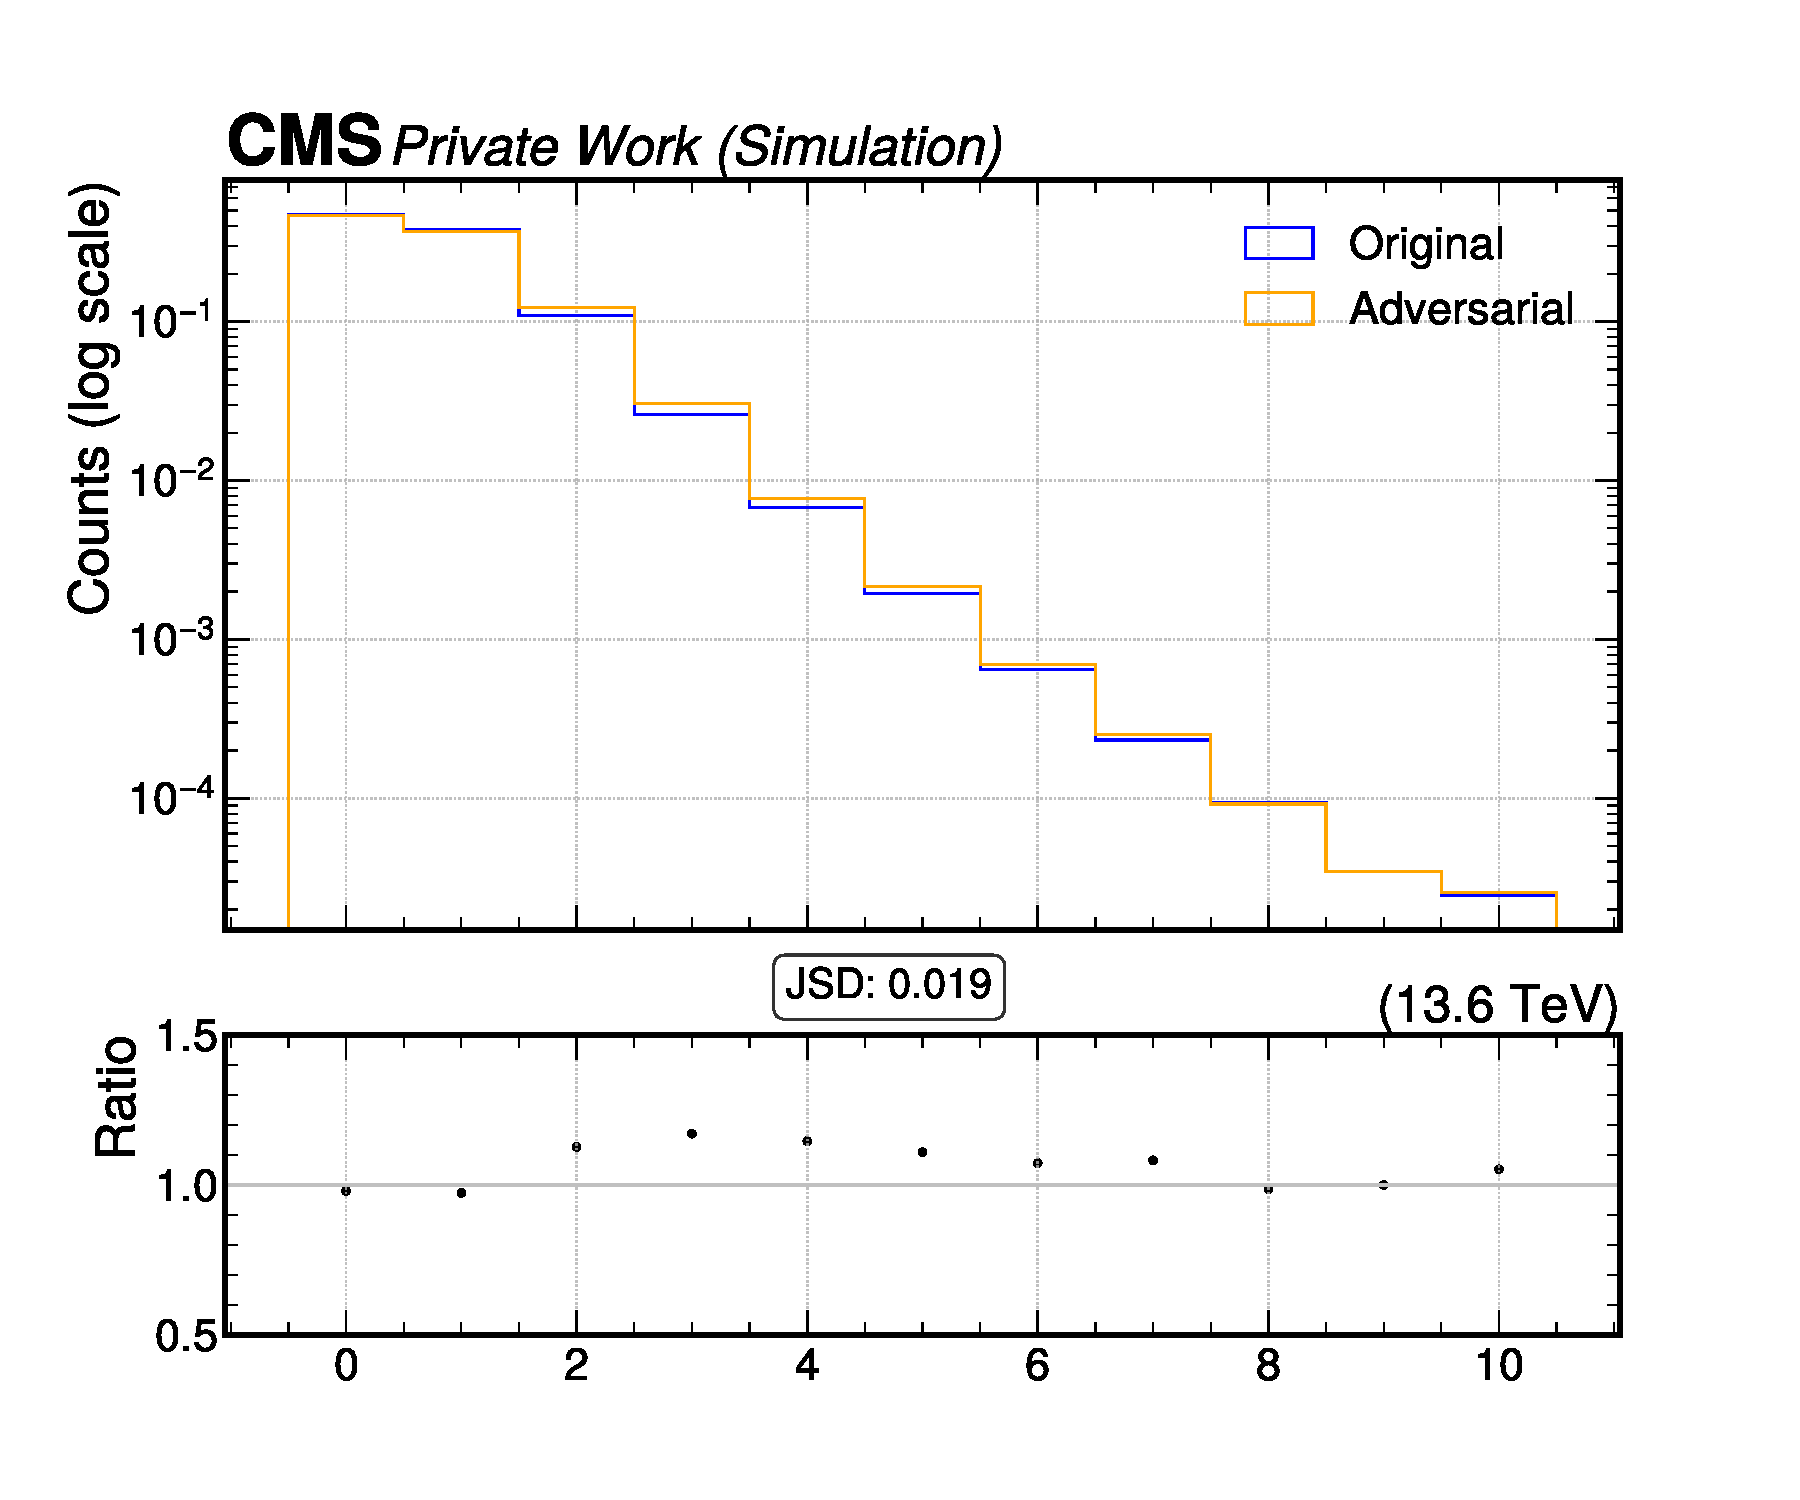
\includegraphics[width=\linewidth]{media/output/features/compare/combined_it_2/cmp_global_features_nsv.pdf}
    \caption*{Input similarity for PIP-PGD(2).}
  \end{subfigure}\hfill
  \begin{subfigure}[t]{0.32\textwidth}
    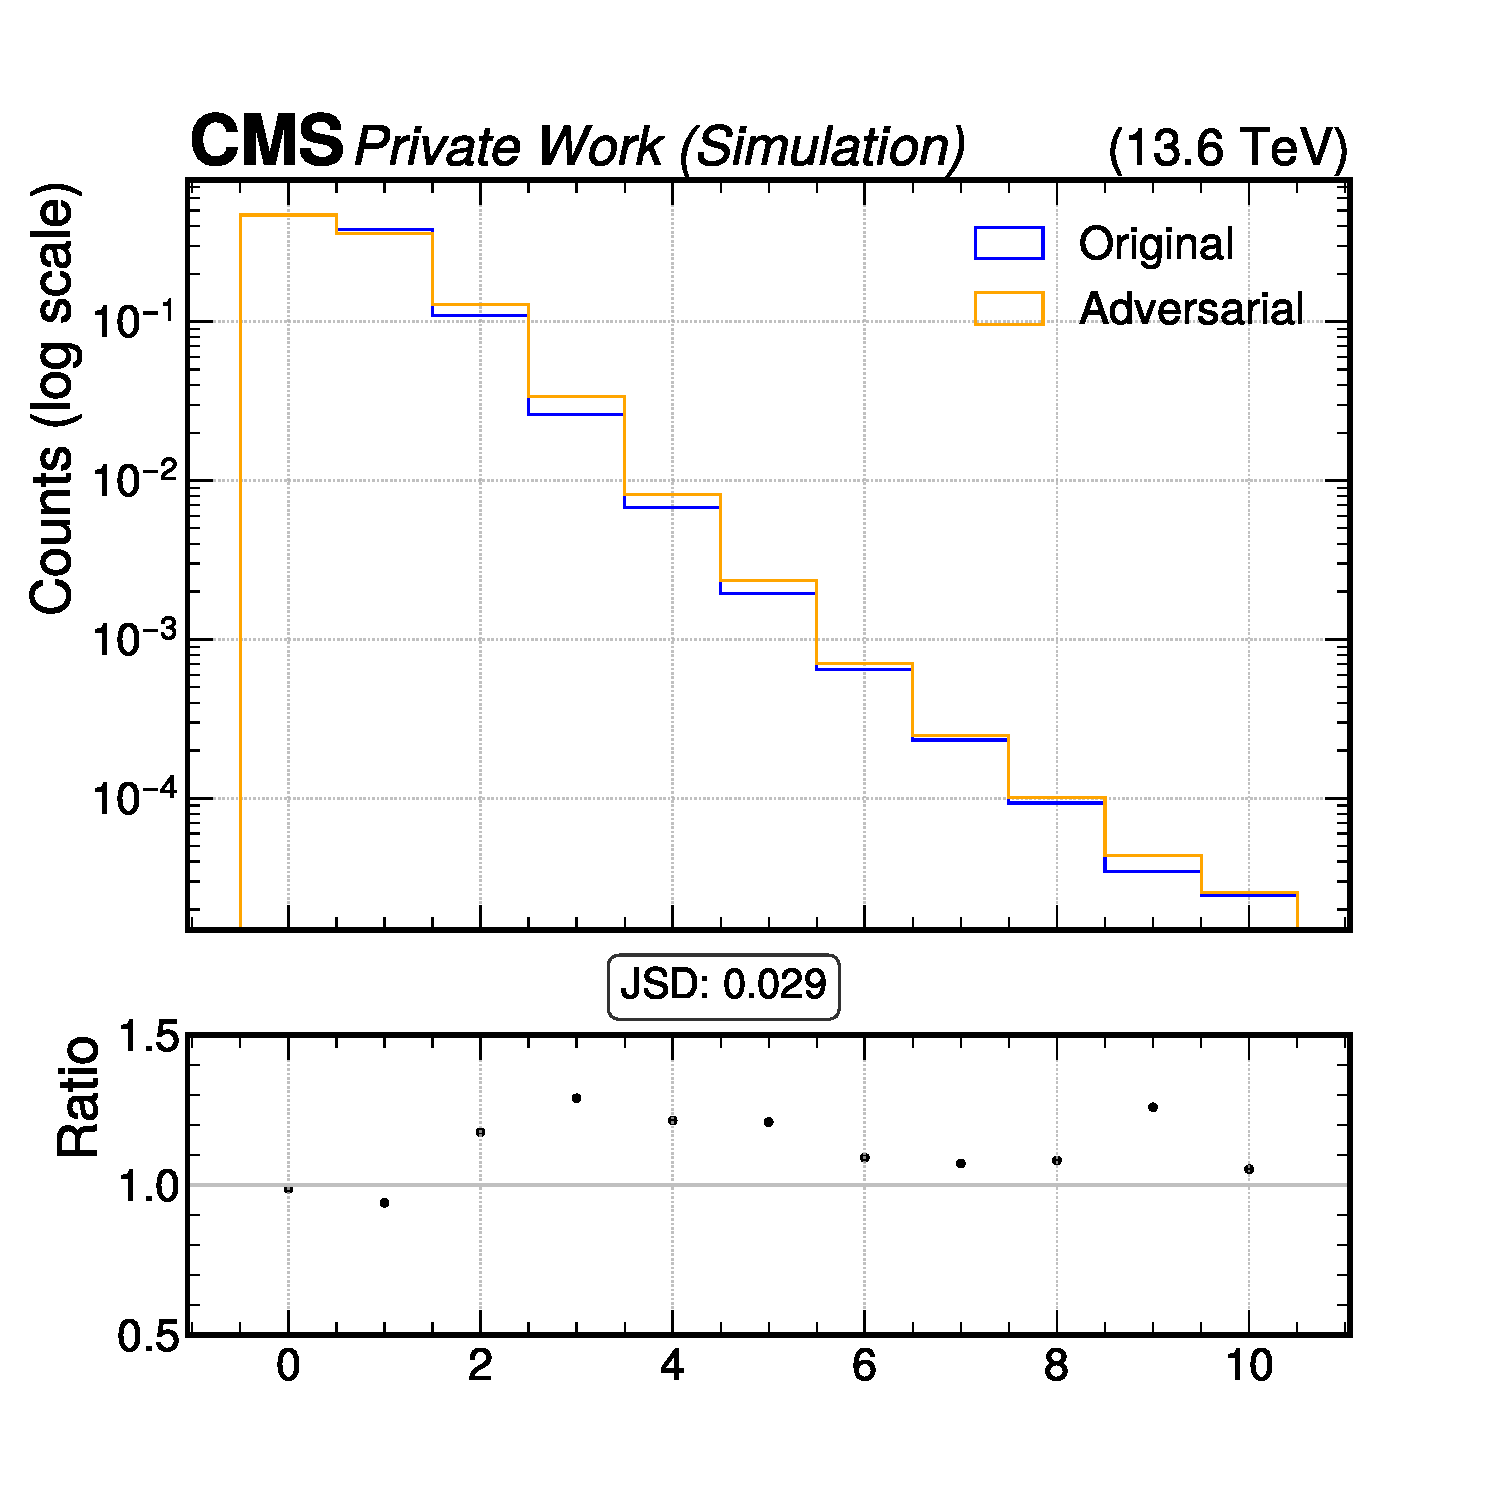
\includegraphics[width=\linewidth]{media/output/features/compare/combined_it_3/cmp_global_features_nsv.pdf}
    \caption*{Input similarity for PIP-PGD(3).}
  \end{subfigure}

  \caption*{Histogram of \texttt{nsv} for multiple iterations of PIP-PGD tested against nominal inputs.}
  \label{fig:combined_input_nsv}
\end{figure}

\begin{figure}[h]
  \centering
  \begin{subfigure}[t]{0.32\textwidth}
    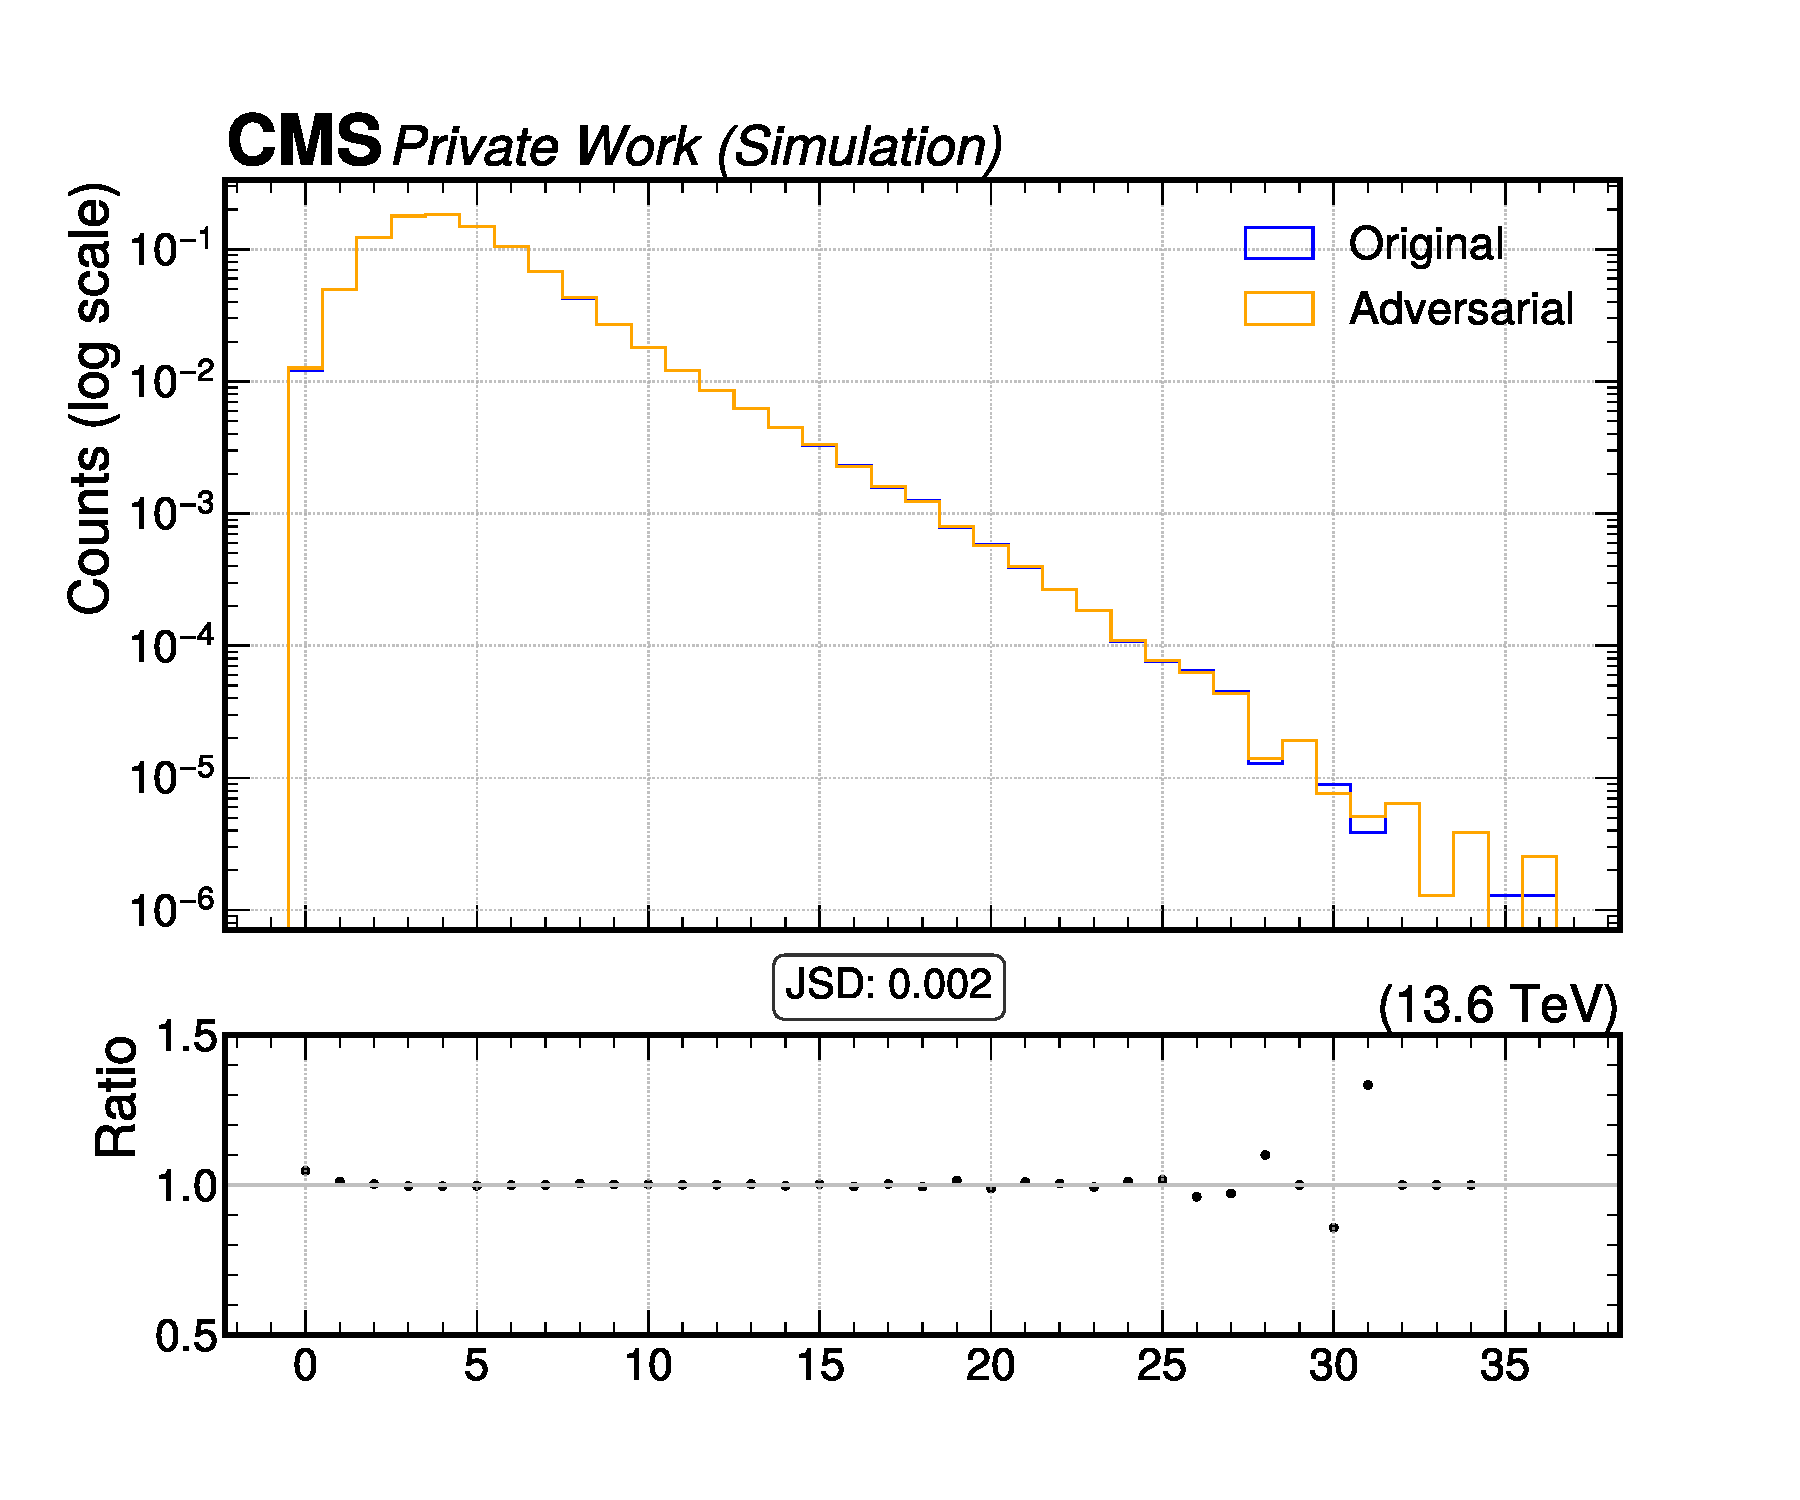
\includegraphics[width=\linewidth]{media/output/features/compare/combined_it_1/cmp_global_features_TagVarCSV_jetNSelectedTracks.pdf}
    \caption*{Input similarity for PIP-PGD(1).}
  \end{subfigure}\hfill
  \begin{subfigure}[t]{0.32\textwidth}
    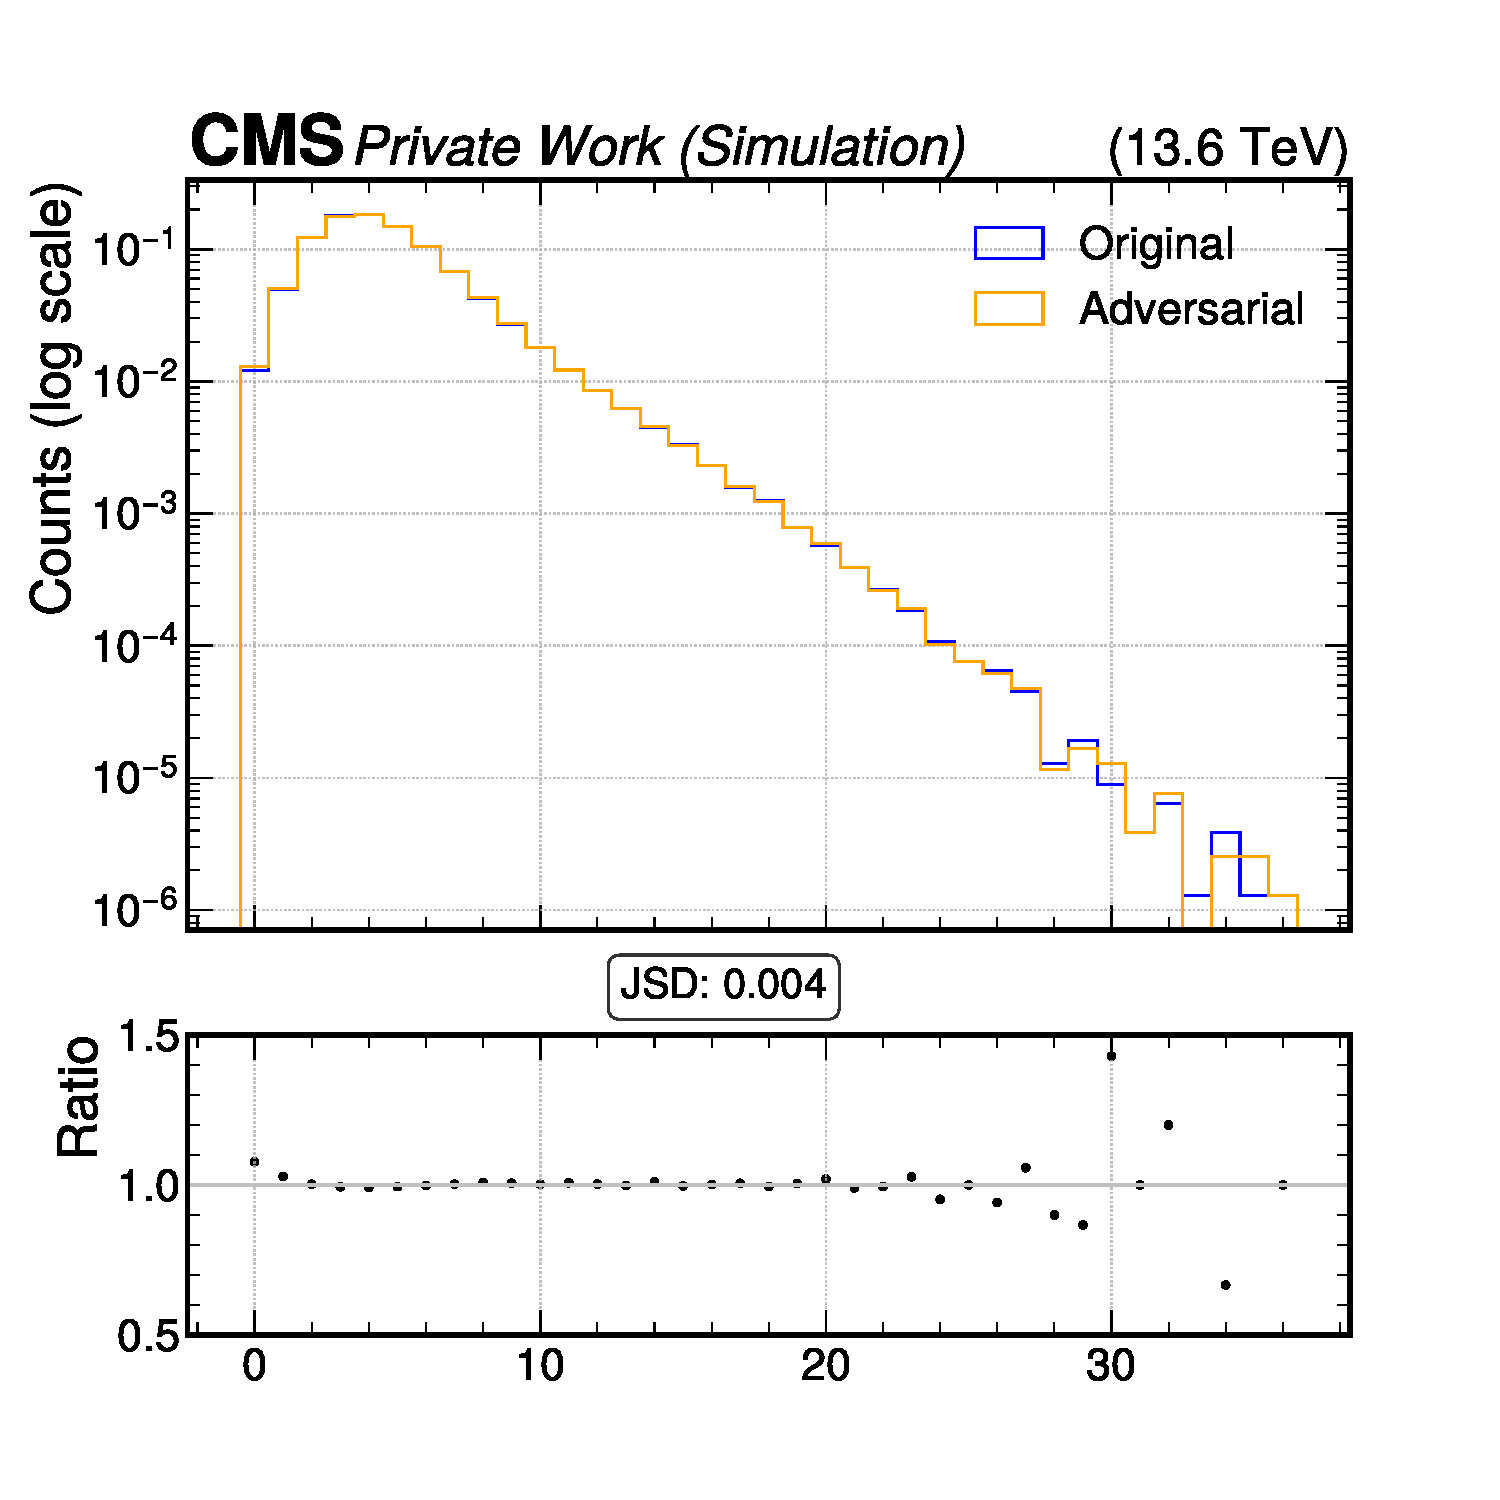
\includegraphics[width=\linewidth]{media/output/features/compare/combined_it_2/cmp_global_features_TagVarCSV_jetNSelectedTracks.pdf}
    \caption*{Input similarity for PIP-PGD(2).}
  \end{subfigure}\hfill
  \begin{subfigure}[t]{0.32\textwidth}
    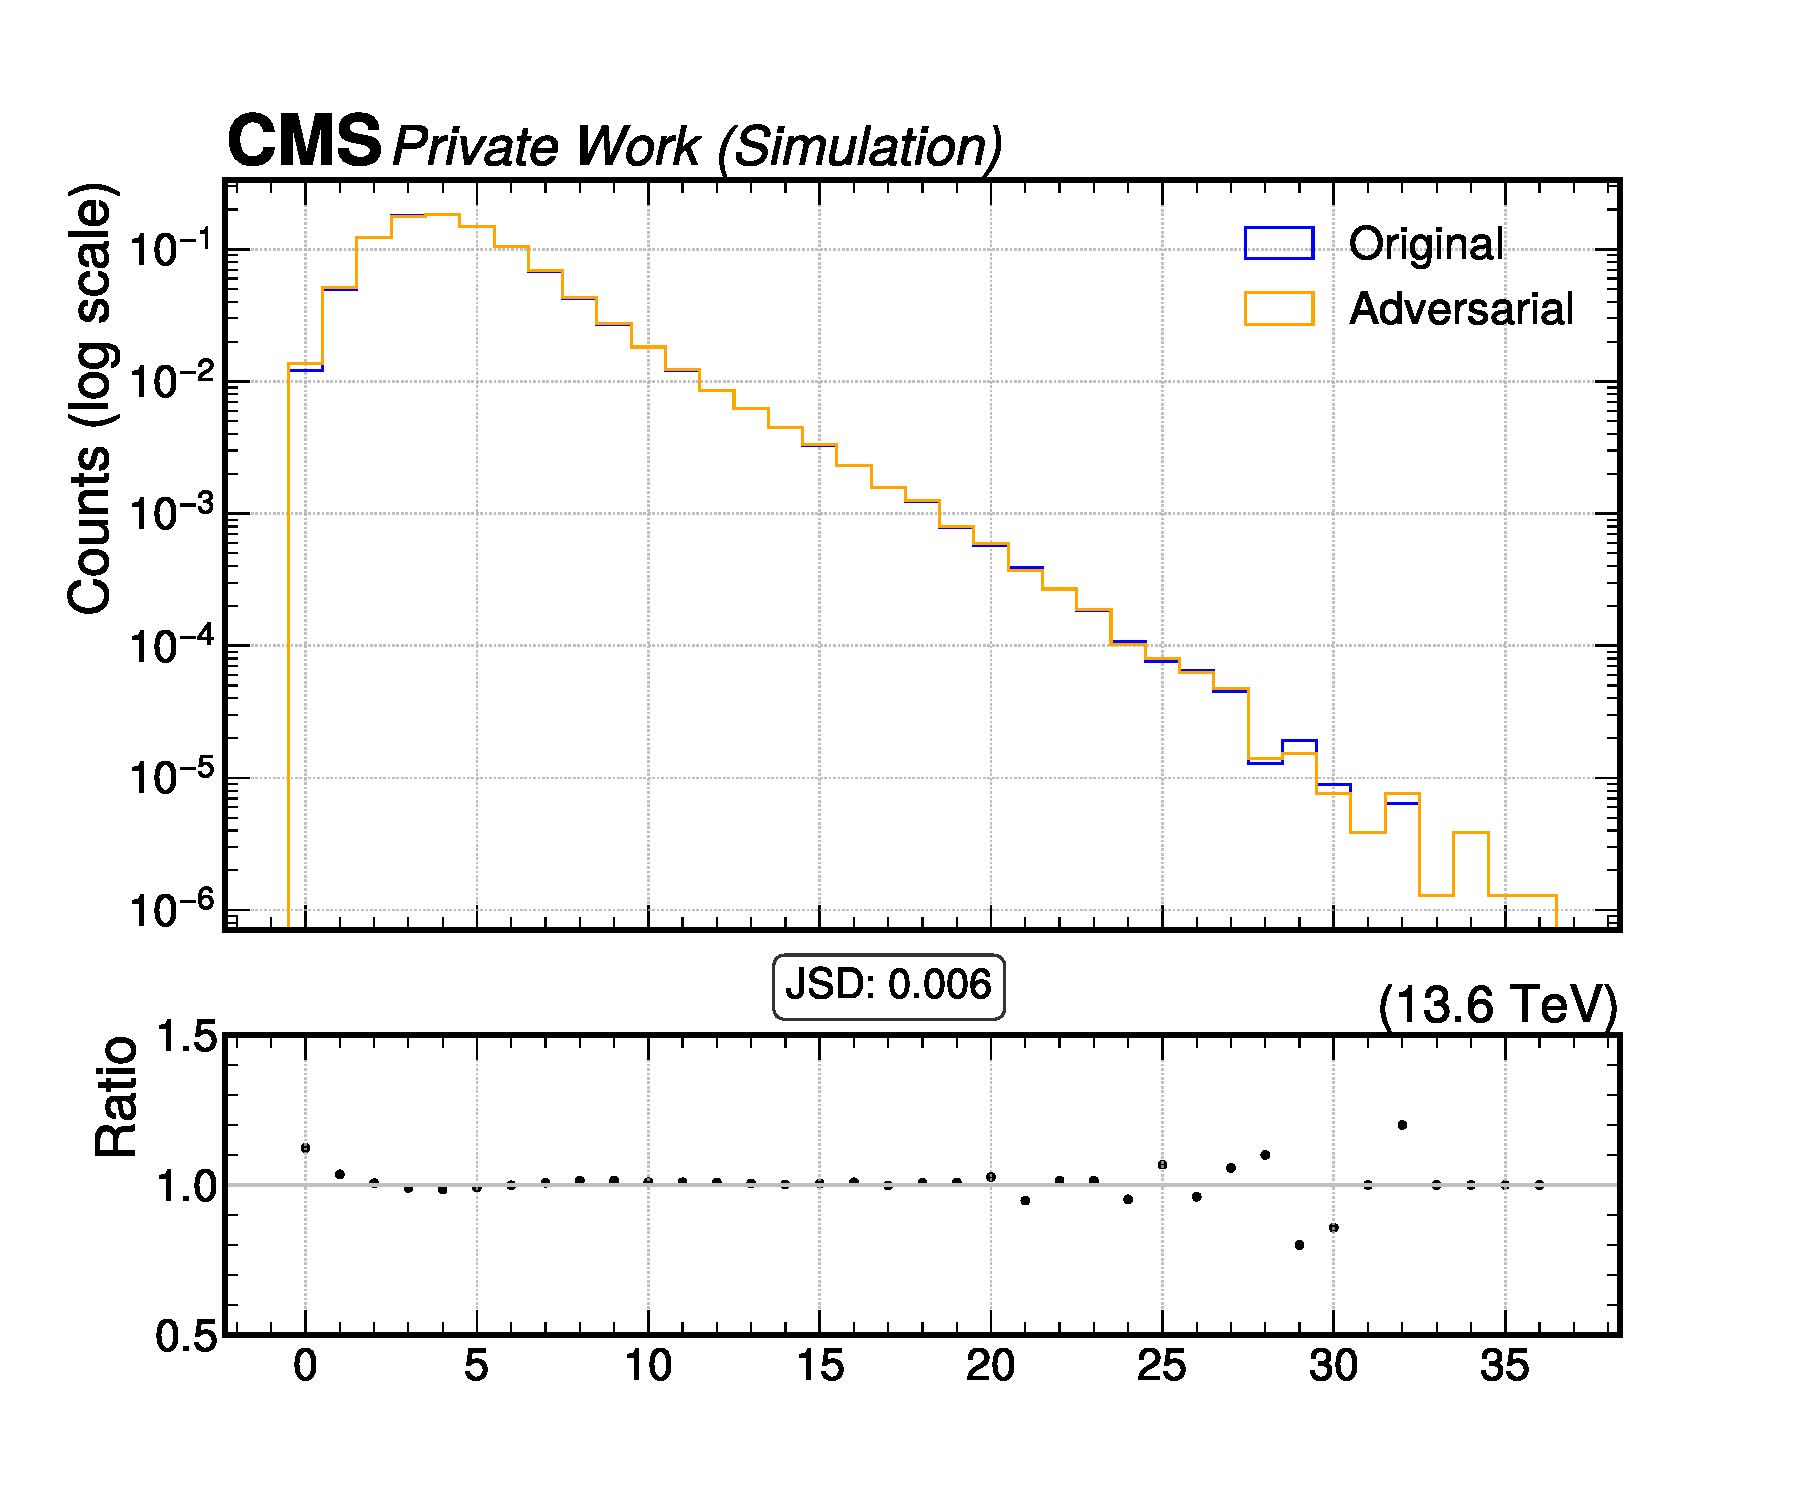
\includegraphics[width=\linewidth]{media/output/features/compare/combined_it_3/cmp_global_features_TagVarCSV_jetNSelectedTracks.pdf}
    \caption*{Input similarity for PIP-PGD(3).}
  \end{subfigure}

  \caption*{Histogram of \texttt{TagVarCSV\_jetNSelectedTracks} for multiple iterations of PIP-PGD tested against nominal inputs.}
  \label{fig:combined_input_TagVarCSV_jetNSelectedTracks}
\end{figure}

\begin{figure}[h]
  \centering
  \begin{subfigure}[t]{0.32\textwidth}
    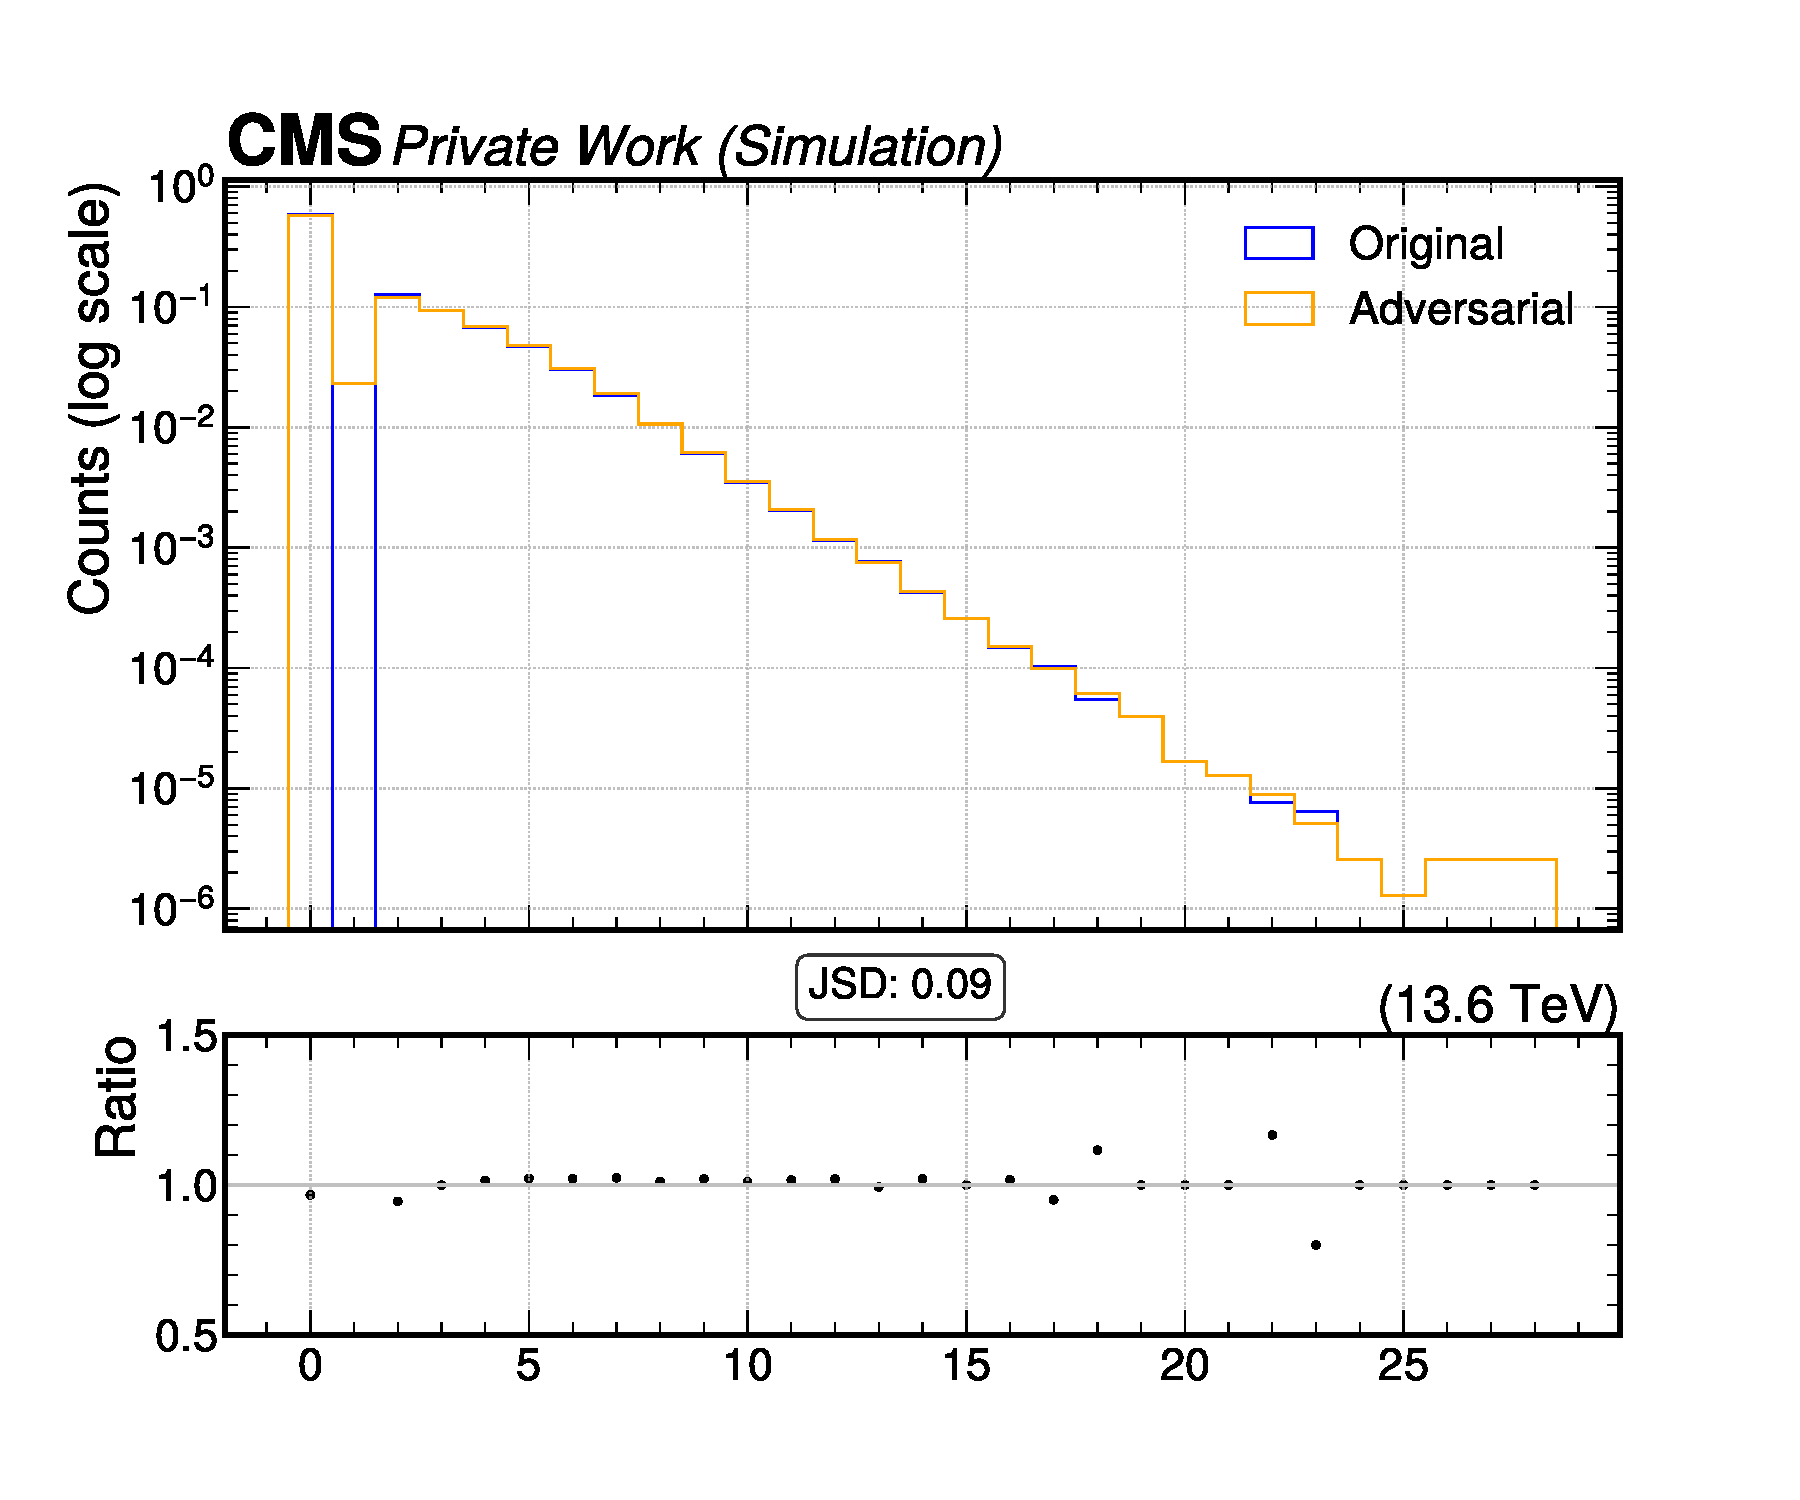
\includegraphics[width=\linewidth]{media/output/features/compare/combined_it_1/cmp_global_features_TagVarCSV_jetNTracksEtaRel.pdf}
    \caption*{Input similarity for PIP-PGD(1).}
  \end{subfigure}\hfill
  \begin{subfigure}[t]{0.32\textwidth}
    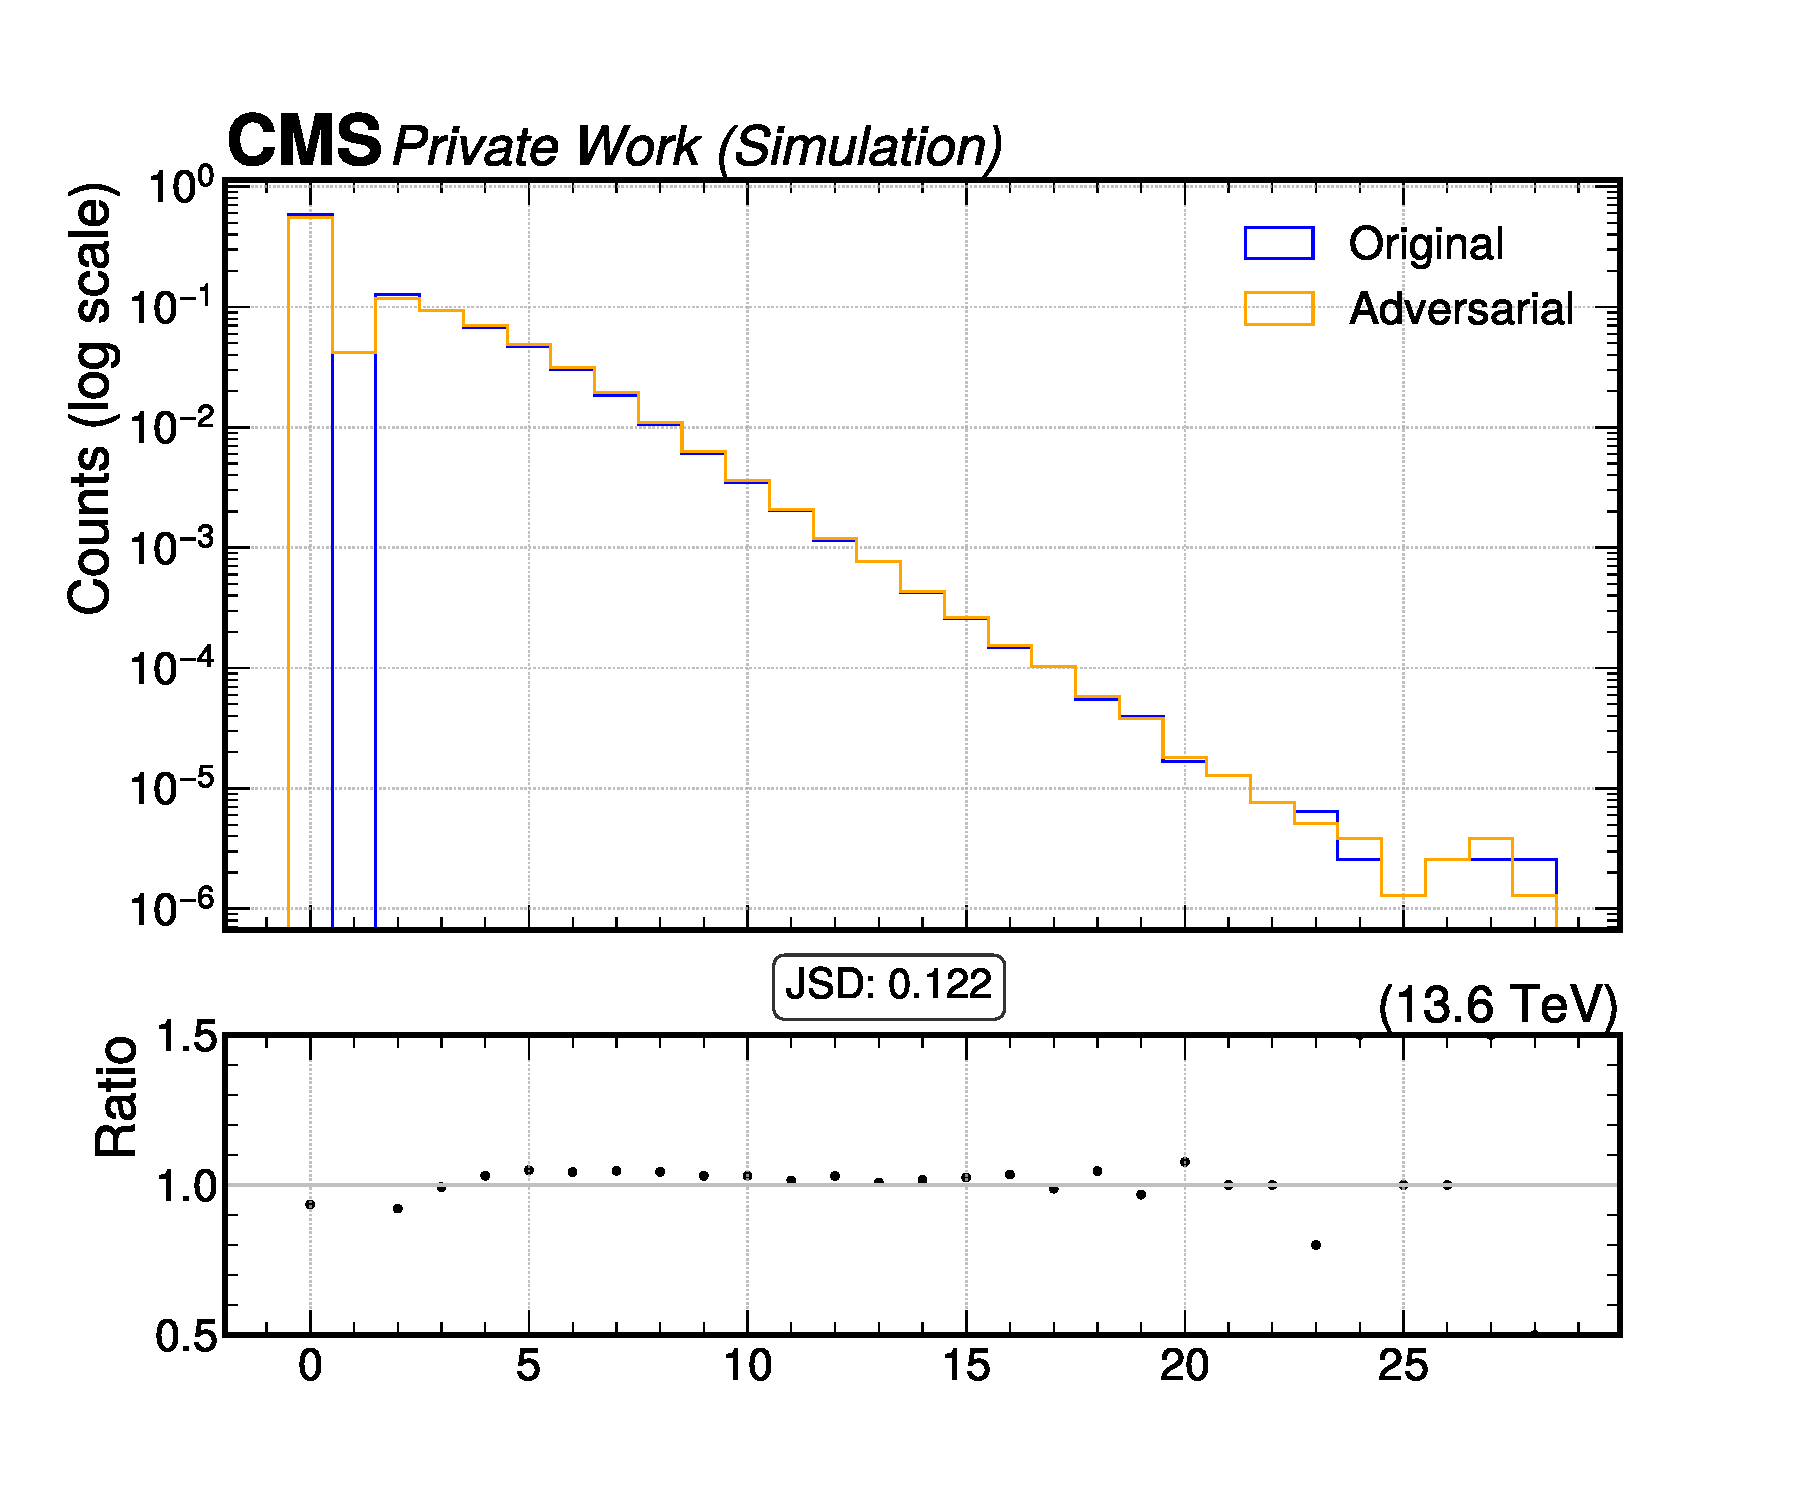
\includegraphics[width=\linewidth]{media/output/features/compare/combined_it_2/cmp_global_features_TagVarCSV_jetNTracksEtaRel.pdf}
    \caption*{Input similarity for PIP-PGD(2).}
  \end{subfigure}\hfill
  \begin{subfigure}[t]{0.32\textwidth}
    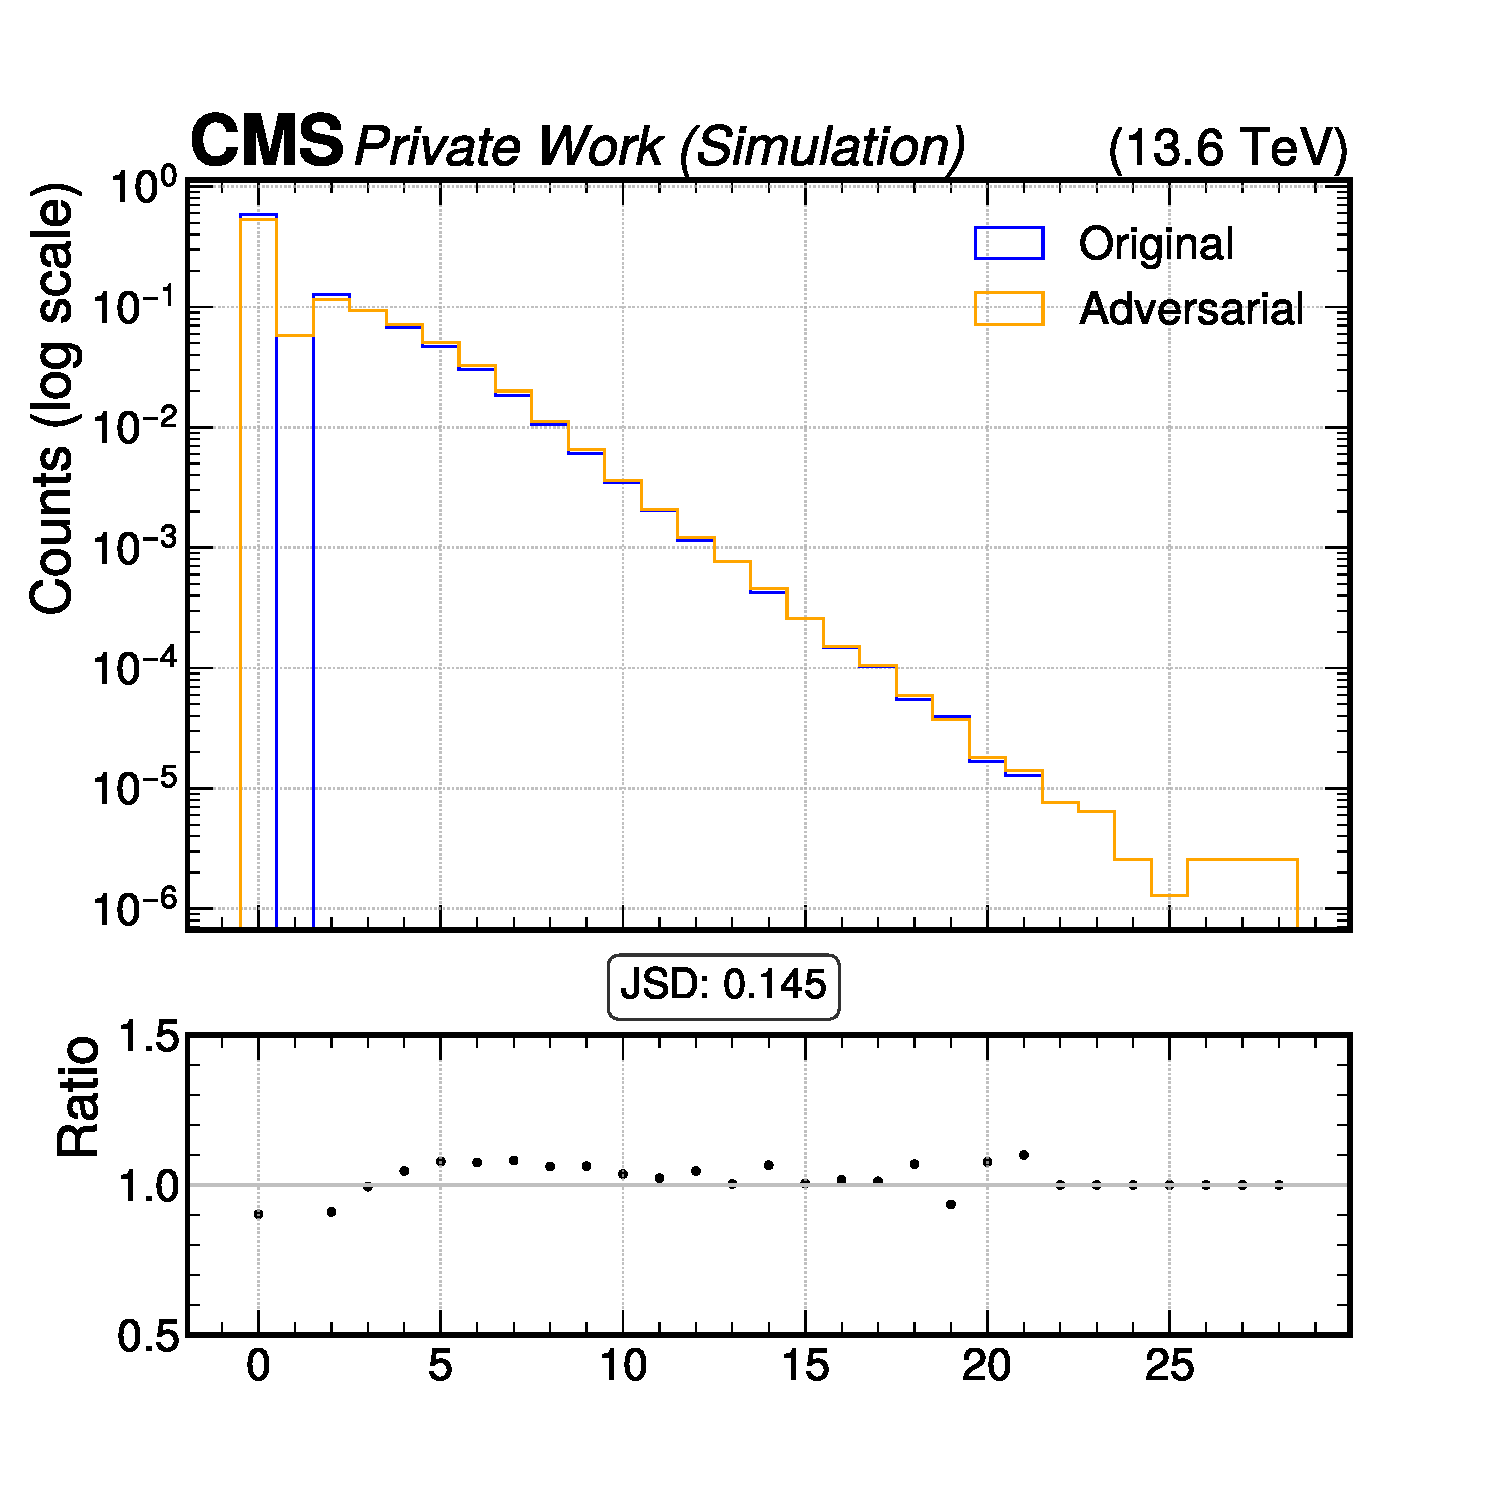
\includegraphics[width=\linewidth]{media/output/features/compare/combined_it_3/cmp_global_features_TagVarCSV_jetNTracksEtaRel.pdf}
    \caption*{Input similarity for PIP-PGD(3).}
  \end{subfigure}

  \caption*{Histogram of \texttt{TagVarCSV\_jetNTracksEtaRel} for multiple iterations of PIP-PGD tested against nominal inputs.}
  \label{fig:combined_input_TagVarCSV_jetNTracksEtaRel}
\end{figure}

\begin{figure}[h]
  \centering
  \begin{subfigure}[t]{0.32\textwidth}
    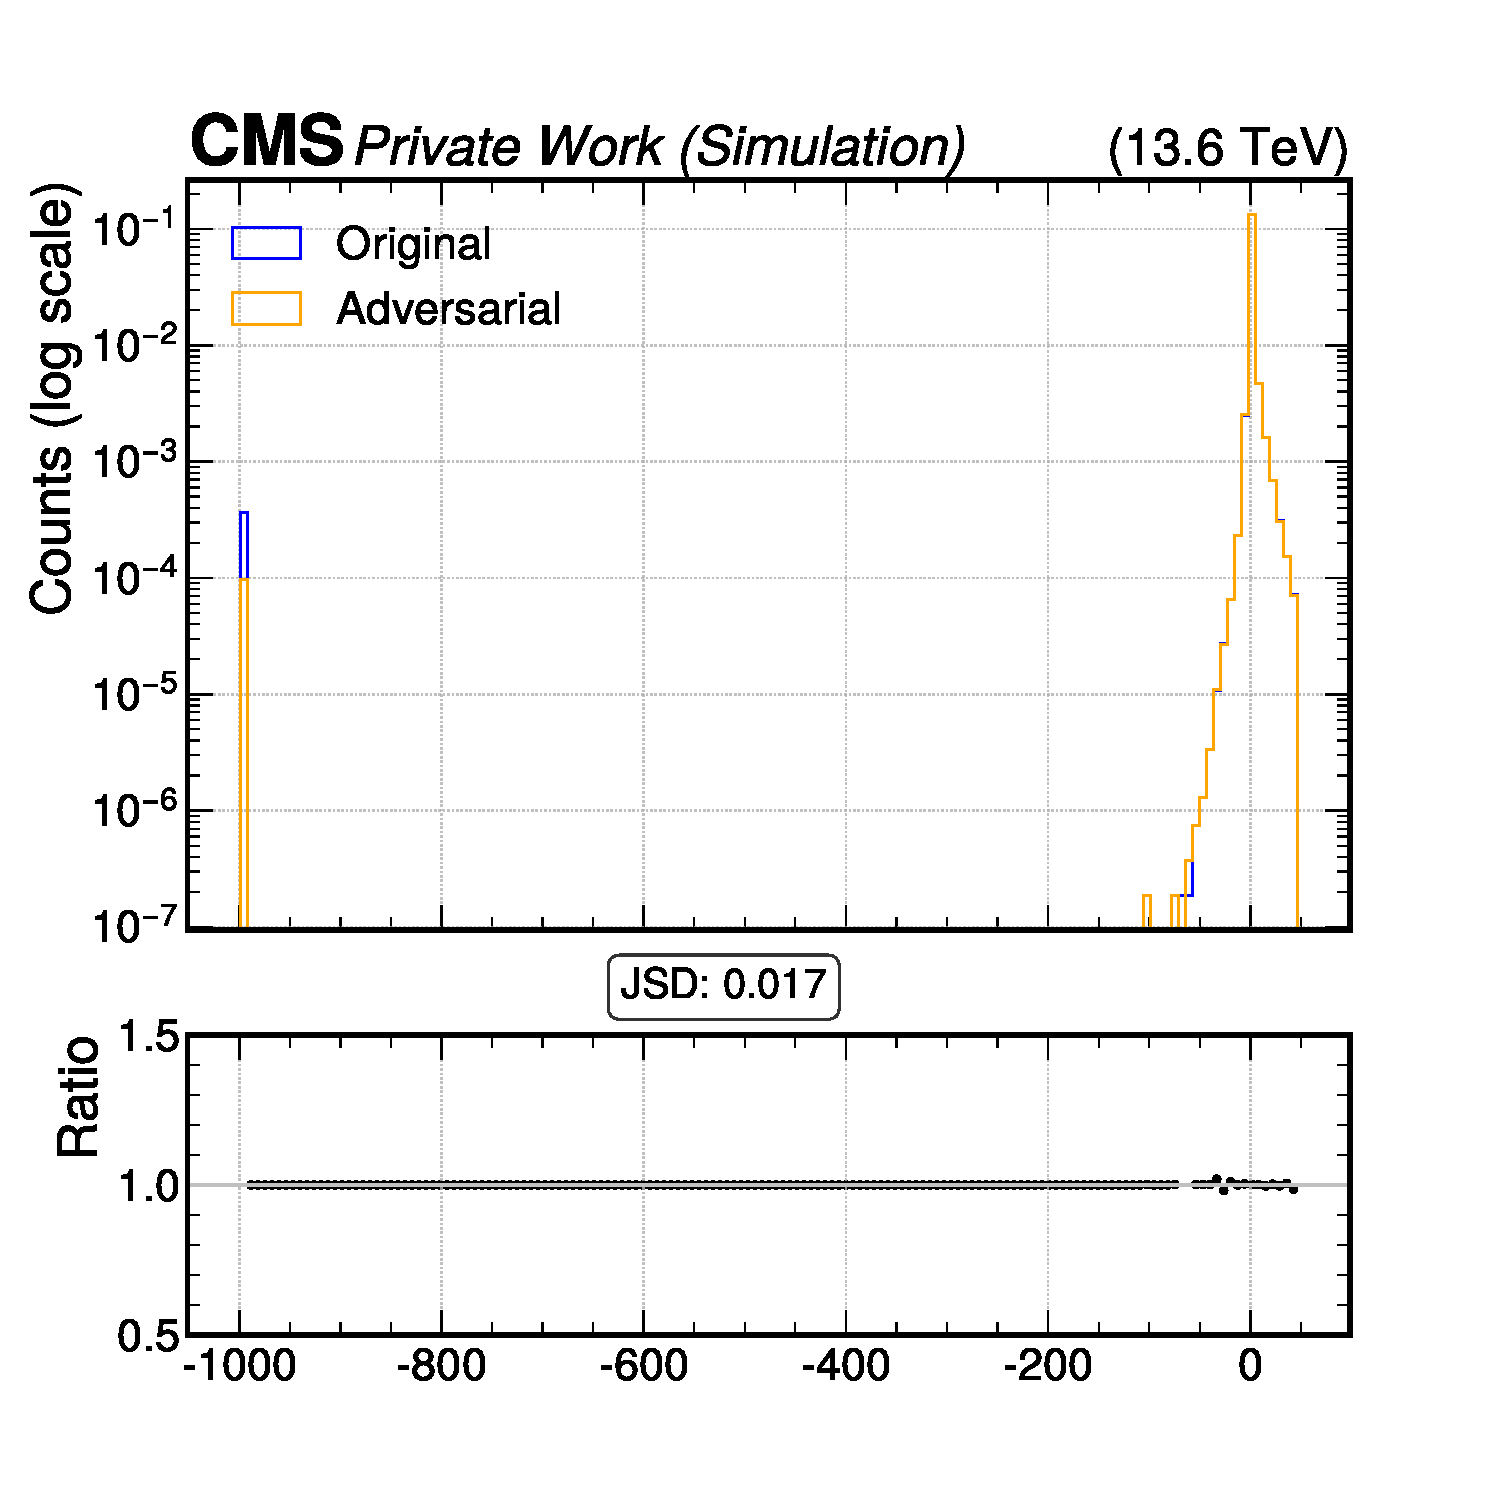
\includegraphics[width=\linewidth]{media/output/features/compare/combined_it_1/cmp_global_features_TagVarCSV_trackSip2dSigAboveCharm.pdf}
    \caption*{Input similarity for PIP-PGD(1).}
  \end{subfigure}\hfill
  \begin{subfigure}[t]{0.32\textwidth}
    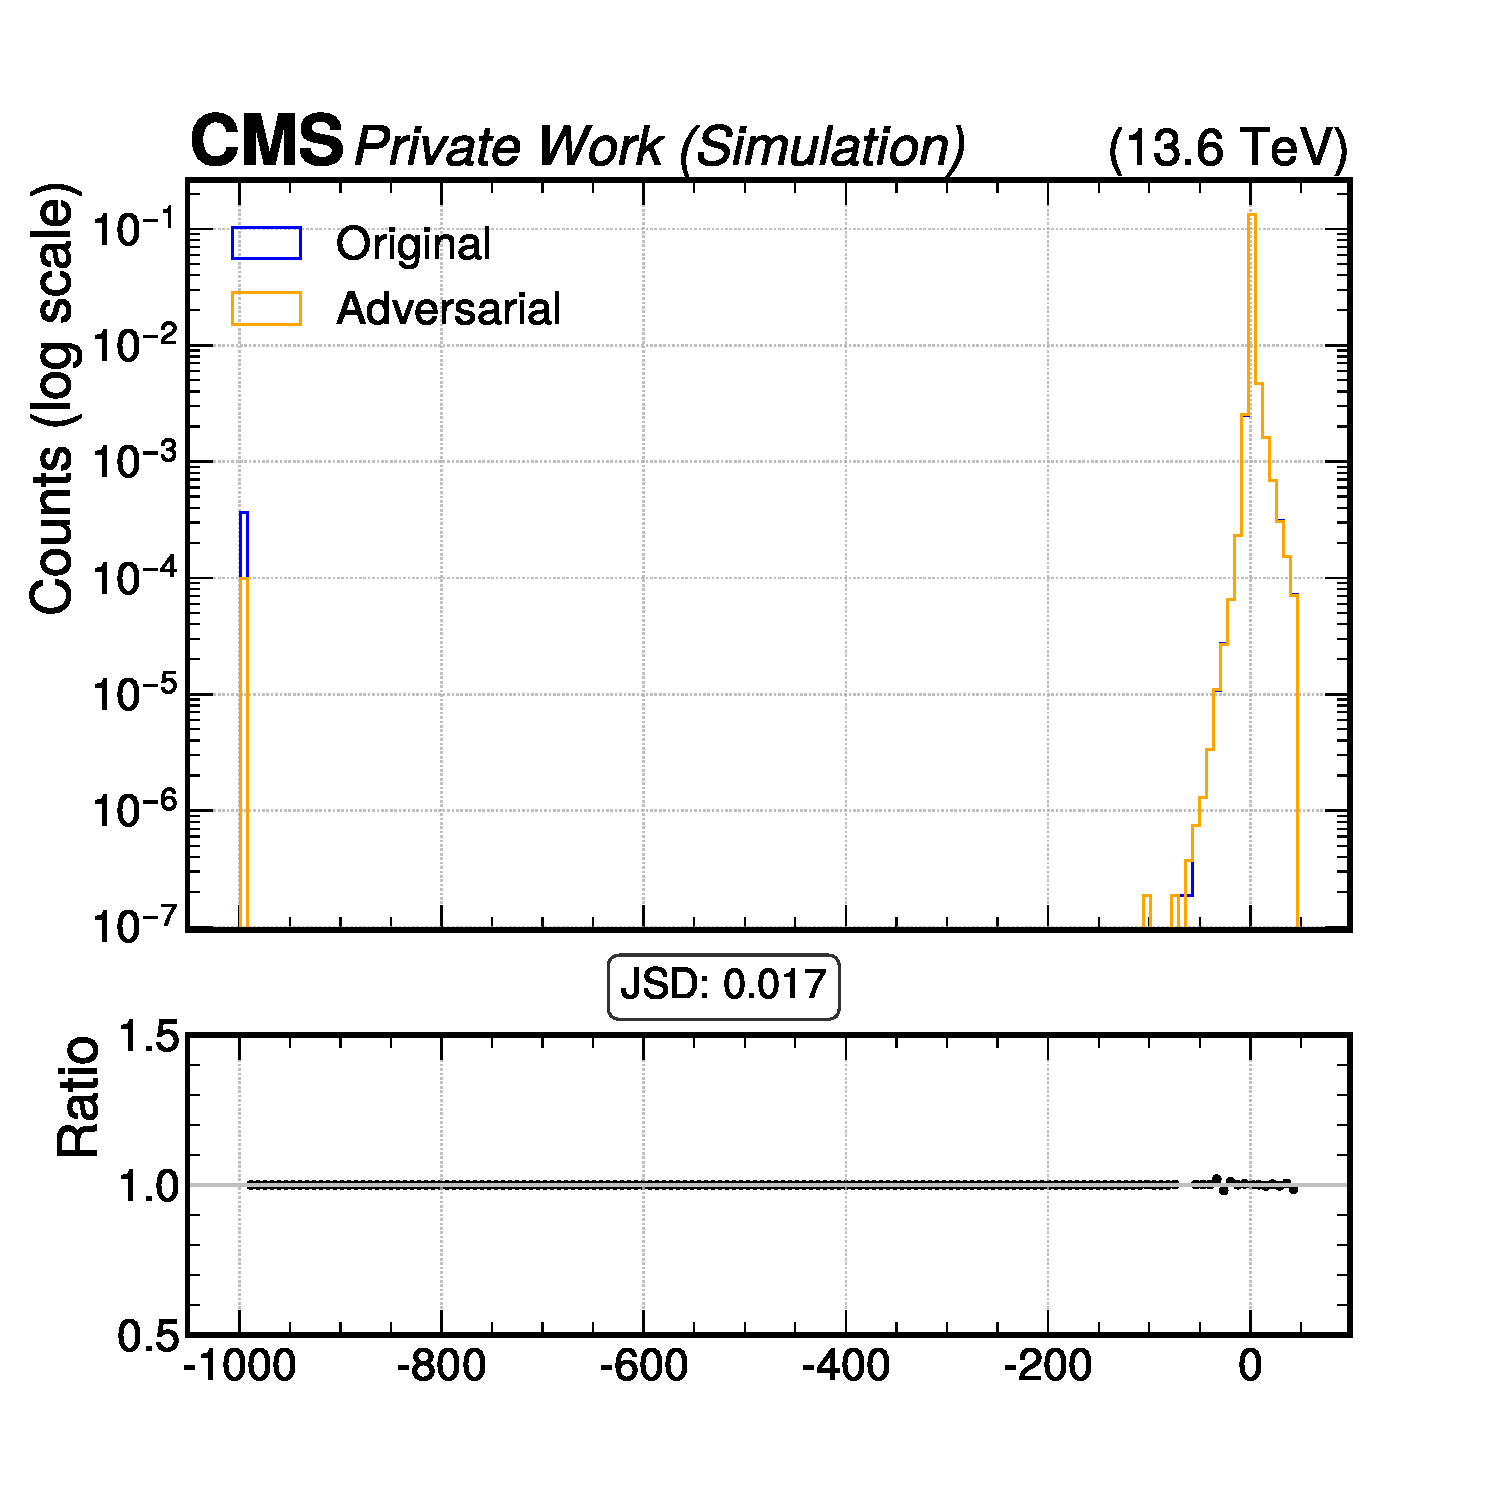
\includegraphics[width=\linewidth]{media/output/features/compare/combined_it_2/cmp_global_features_TagVarCSV_trackSip2dSigAboveCharm.pdf}
    \caption*{Input similarity for PIP-PGD(2).}
  \end{subfigure}\hfill
  \begin{subfigure}[t]{0.32\textwidth}
    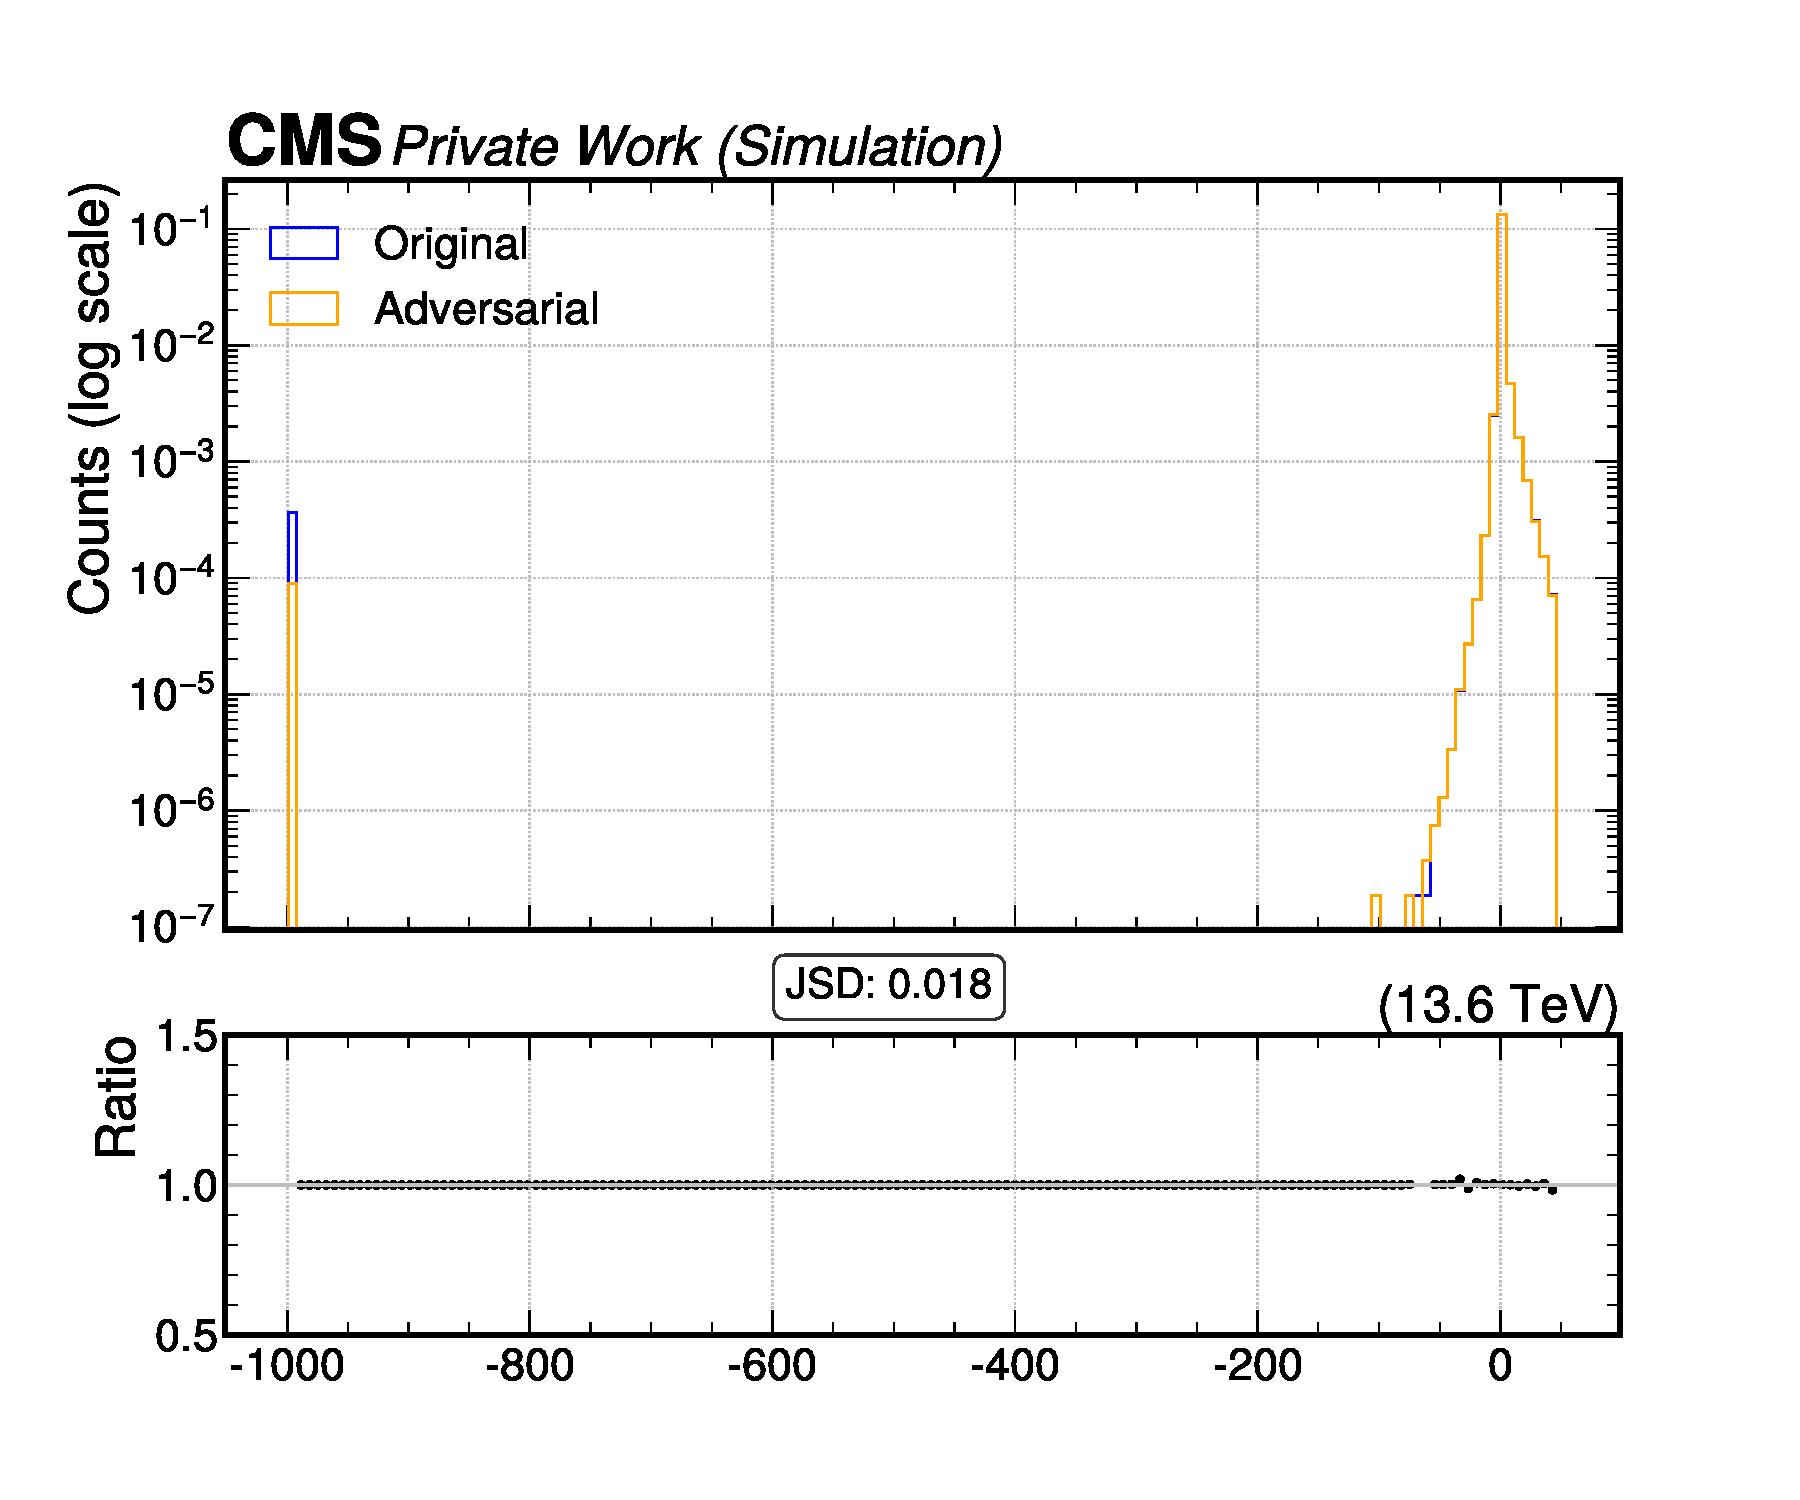
\includegraphics[width=\linewidth]{media/output/features/compare/combined_it_3/cmp_global_features_TagVarCSV_trackSip2dSigAboveCharm.pdf}
    \caption*{Input similarity for PIP-PGD(3).}
  \end{subfigure}

  \caption*{Histogram of \texttt{TagVarCSV\_trackSip2dSigAboveCharm} for multiple iterations of PIP-PGD tested against nominal inputs.}
  \label{fig:combined_input_TagVarCSV_trackSip2dSigAboveCharm}
\end{figure}

\begin{figure}[h]
  \centering
  \begin{subfigure}[t]{0.32\textwidth}
    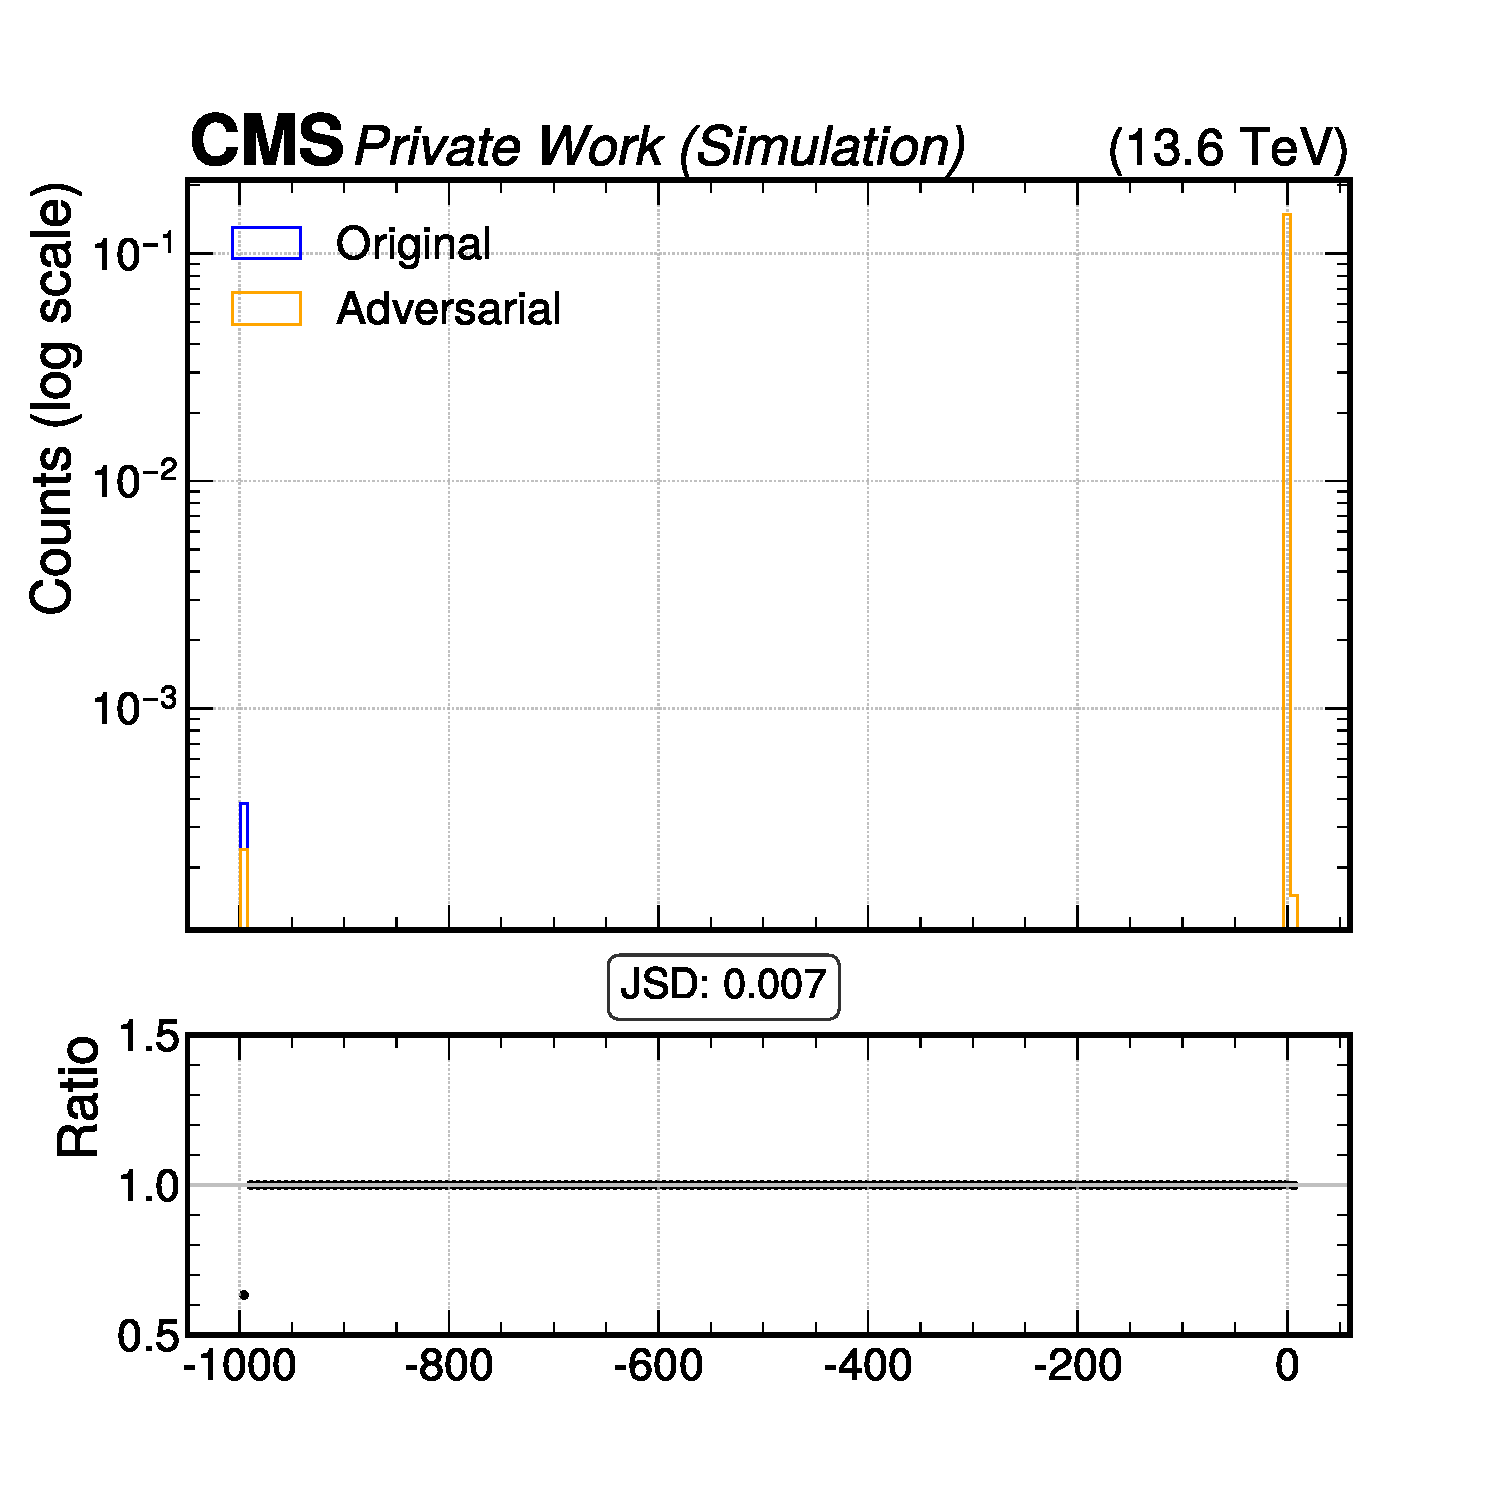
\includegraphics[width=\linewidth]{media/output/features/compare/combined_it_1/cmp_global_features_TagVarCSV_trackSumJetDeltaR.pdf}
    \caption*{Input similarity for PIP-PGD(1).}
  \end{subfigure}\hfill
  \begin{subfigure}[t]{0.32\textwidth}
    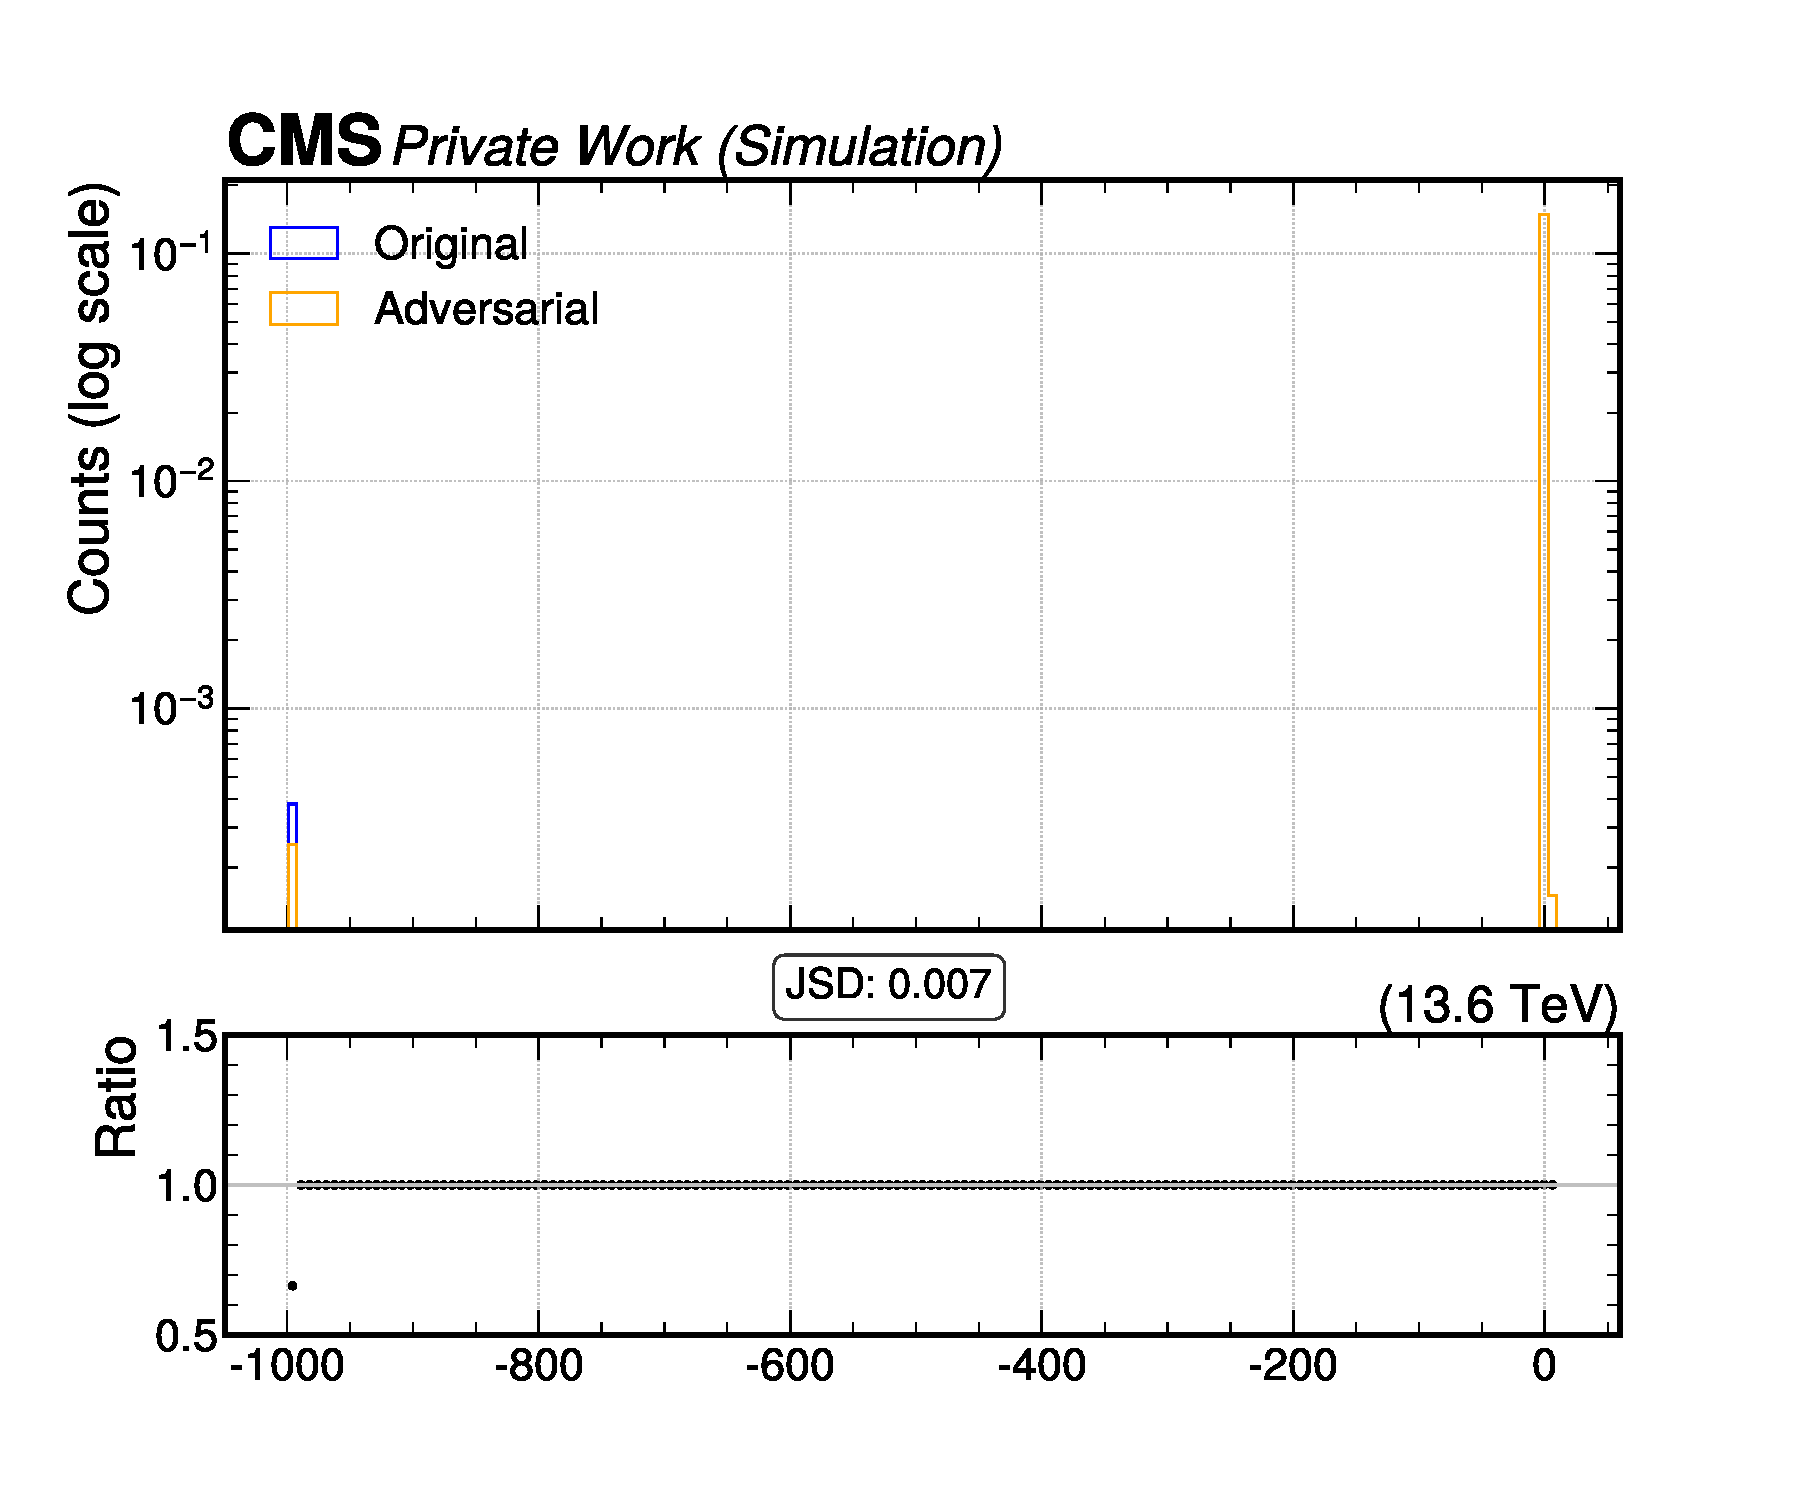
\includegraphics[width=\linewidth]{media/output/features/compare/combined_it_2/cmp_global_features_TagVarCSV_trackSumJetDeltaR.pdf}
    \caption*{Input similarity for PIP-PGD(2).}
  \end{subfigure}\hfill
  \begin{subfigure}[t]{0.32\textwidth}
    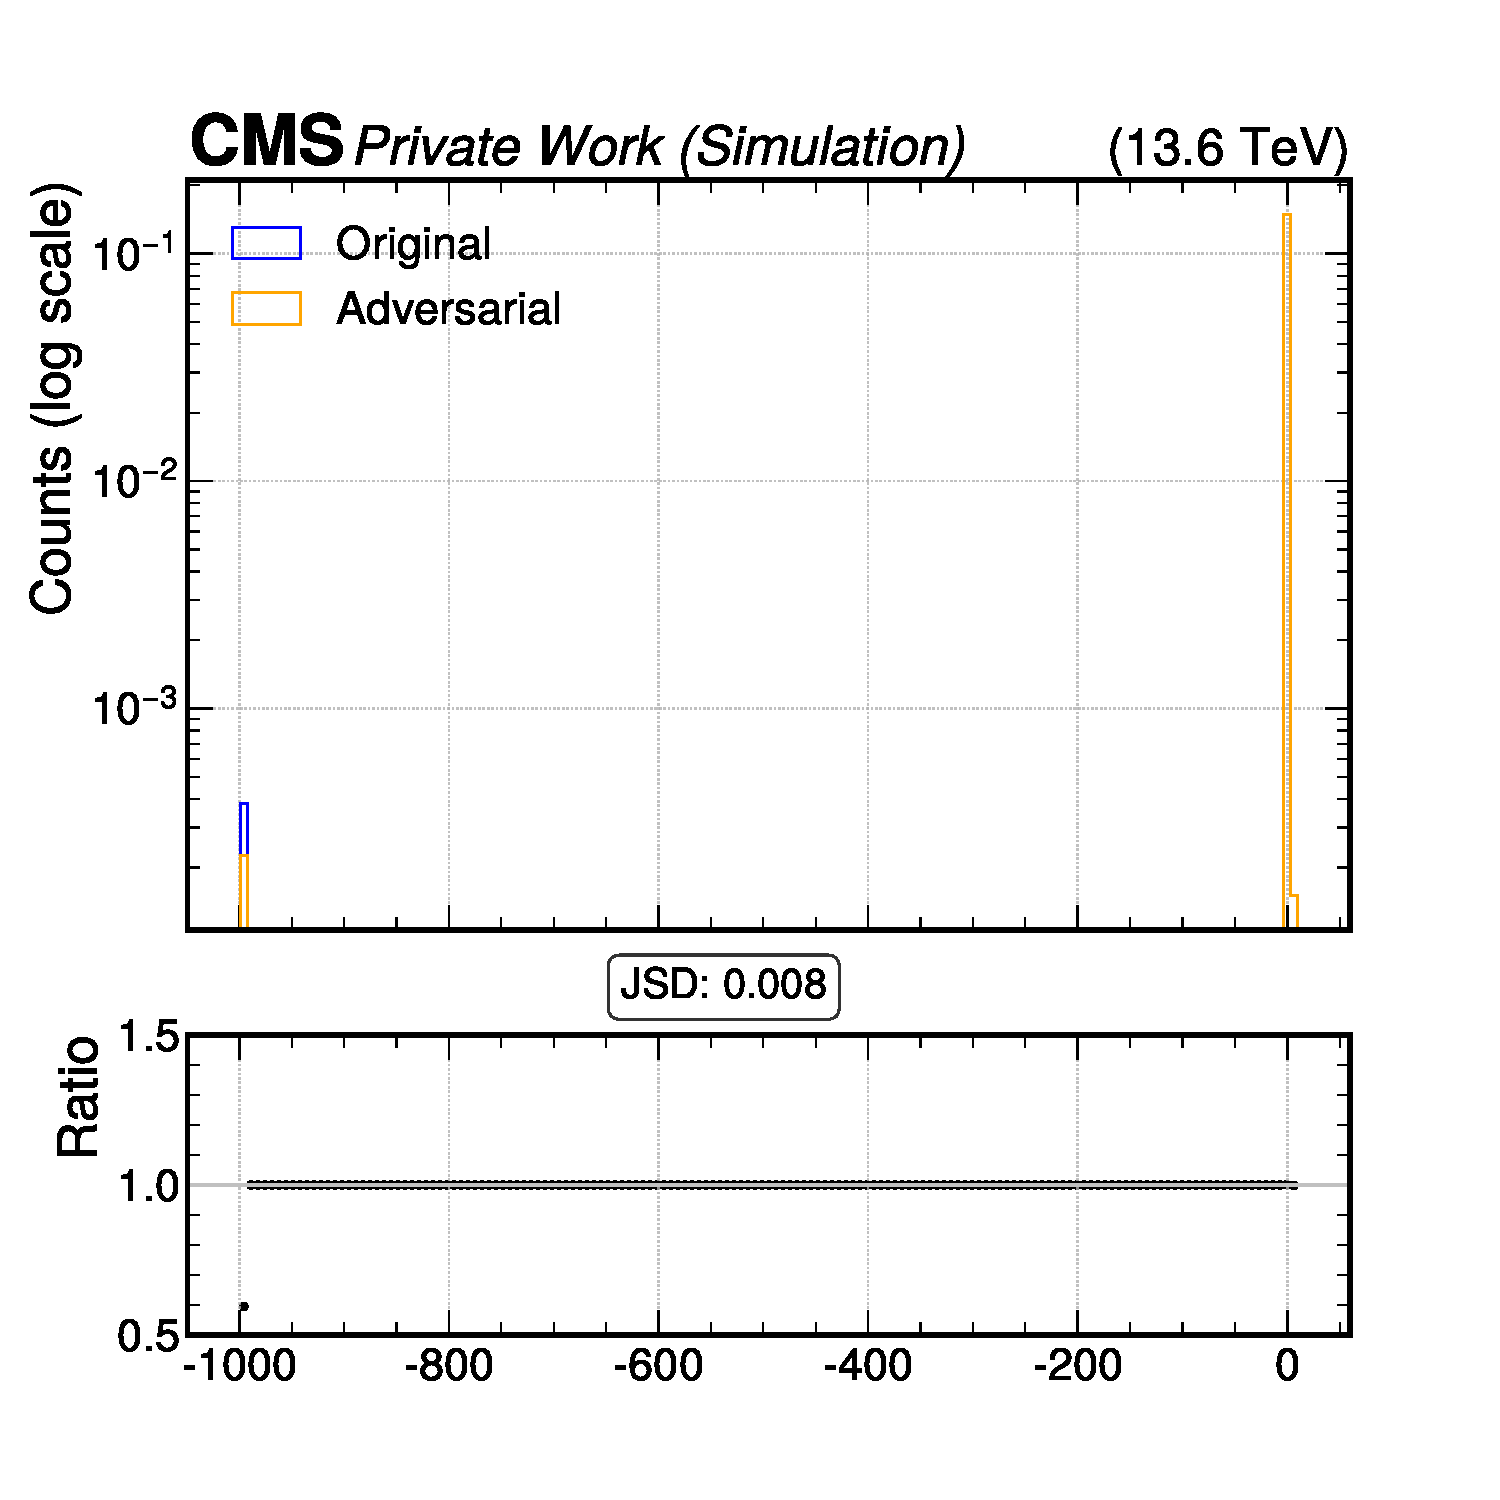
\includegraphics[width=\linewidth]{media/output/features/compare/combined_it_3/cmp_global_features_TagVarCSV_trackSumJetDeltaR.pdf}
    \caption*{Input similarity for PIP-PGD(3).}
  \end{subfigure}

  \caption*{Histogram of \texttt{TagVarCSV\_trackSumJetDeltaR} for multiple iterations of PIP-PGD tested against nominal inputs.}
  \label{fig:combined_input_TagVarCSV_trackSumJetDeltaR}
\end{figure}

\begin{figure}[h]
  \centering
  \begin{subfigure}[t]{0.32\textwidth}
    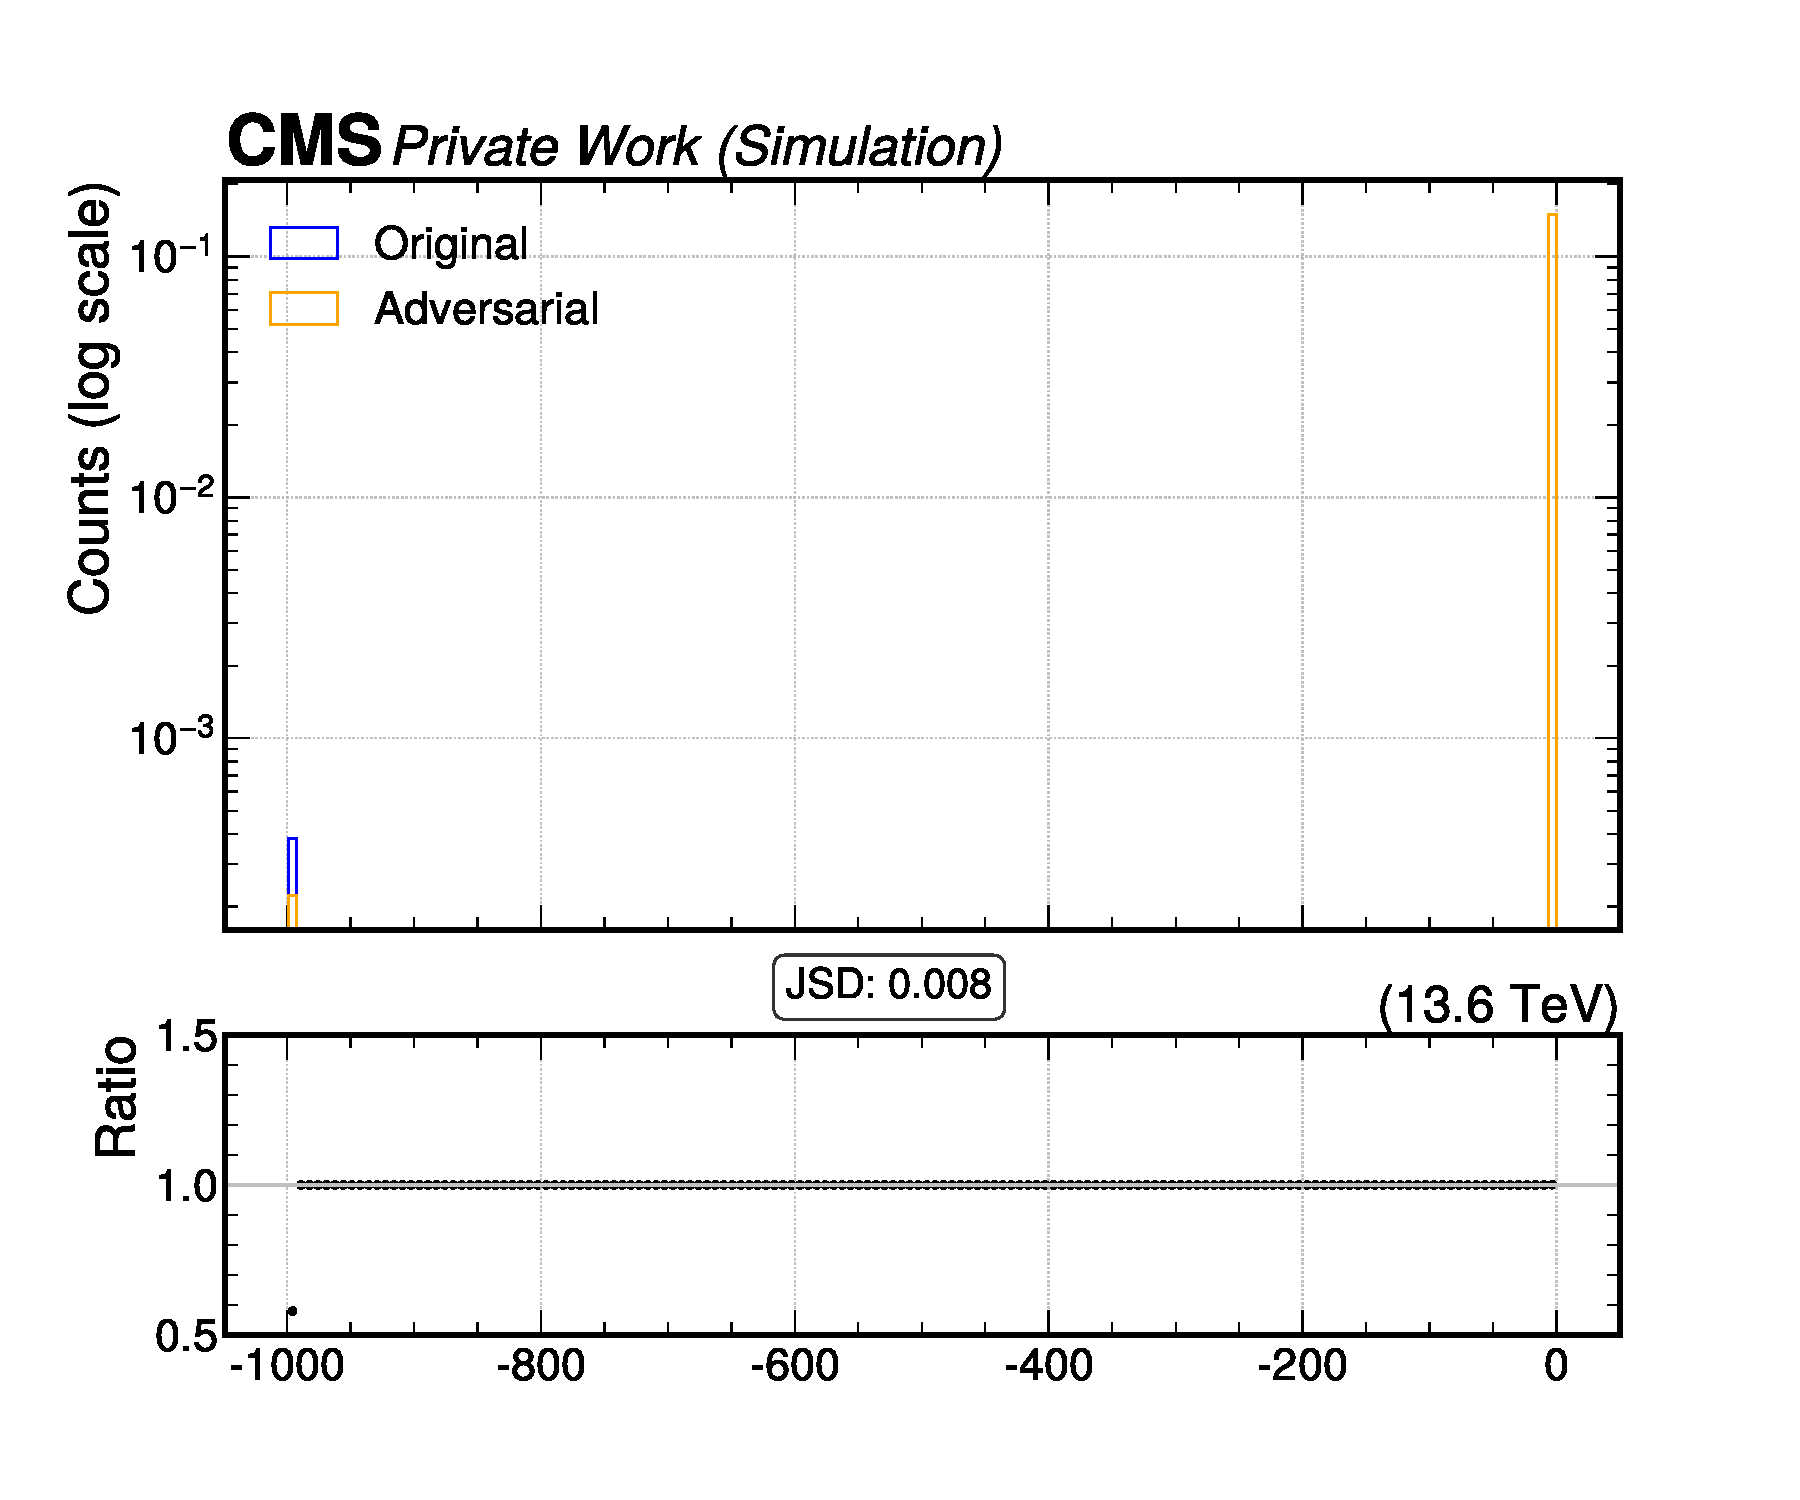
\includegraphics[width=\linewidth]{media/output/features/compare/combined_it_1/cmp_global_features_TagVarCSV_trackSip2dValAboveCharm.pdf}
    \caption*{Input similarity for PIP-PGD(1).}
  \end{subfigure}\hfill
  \begin{subfigure}[t]{0.32\textwidth}
    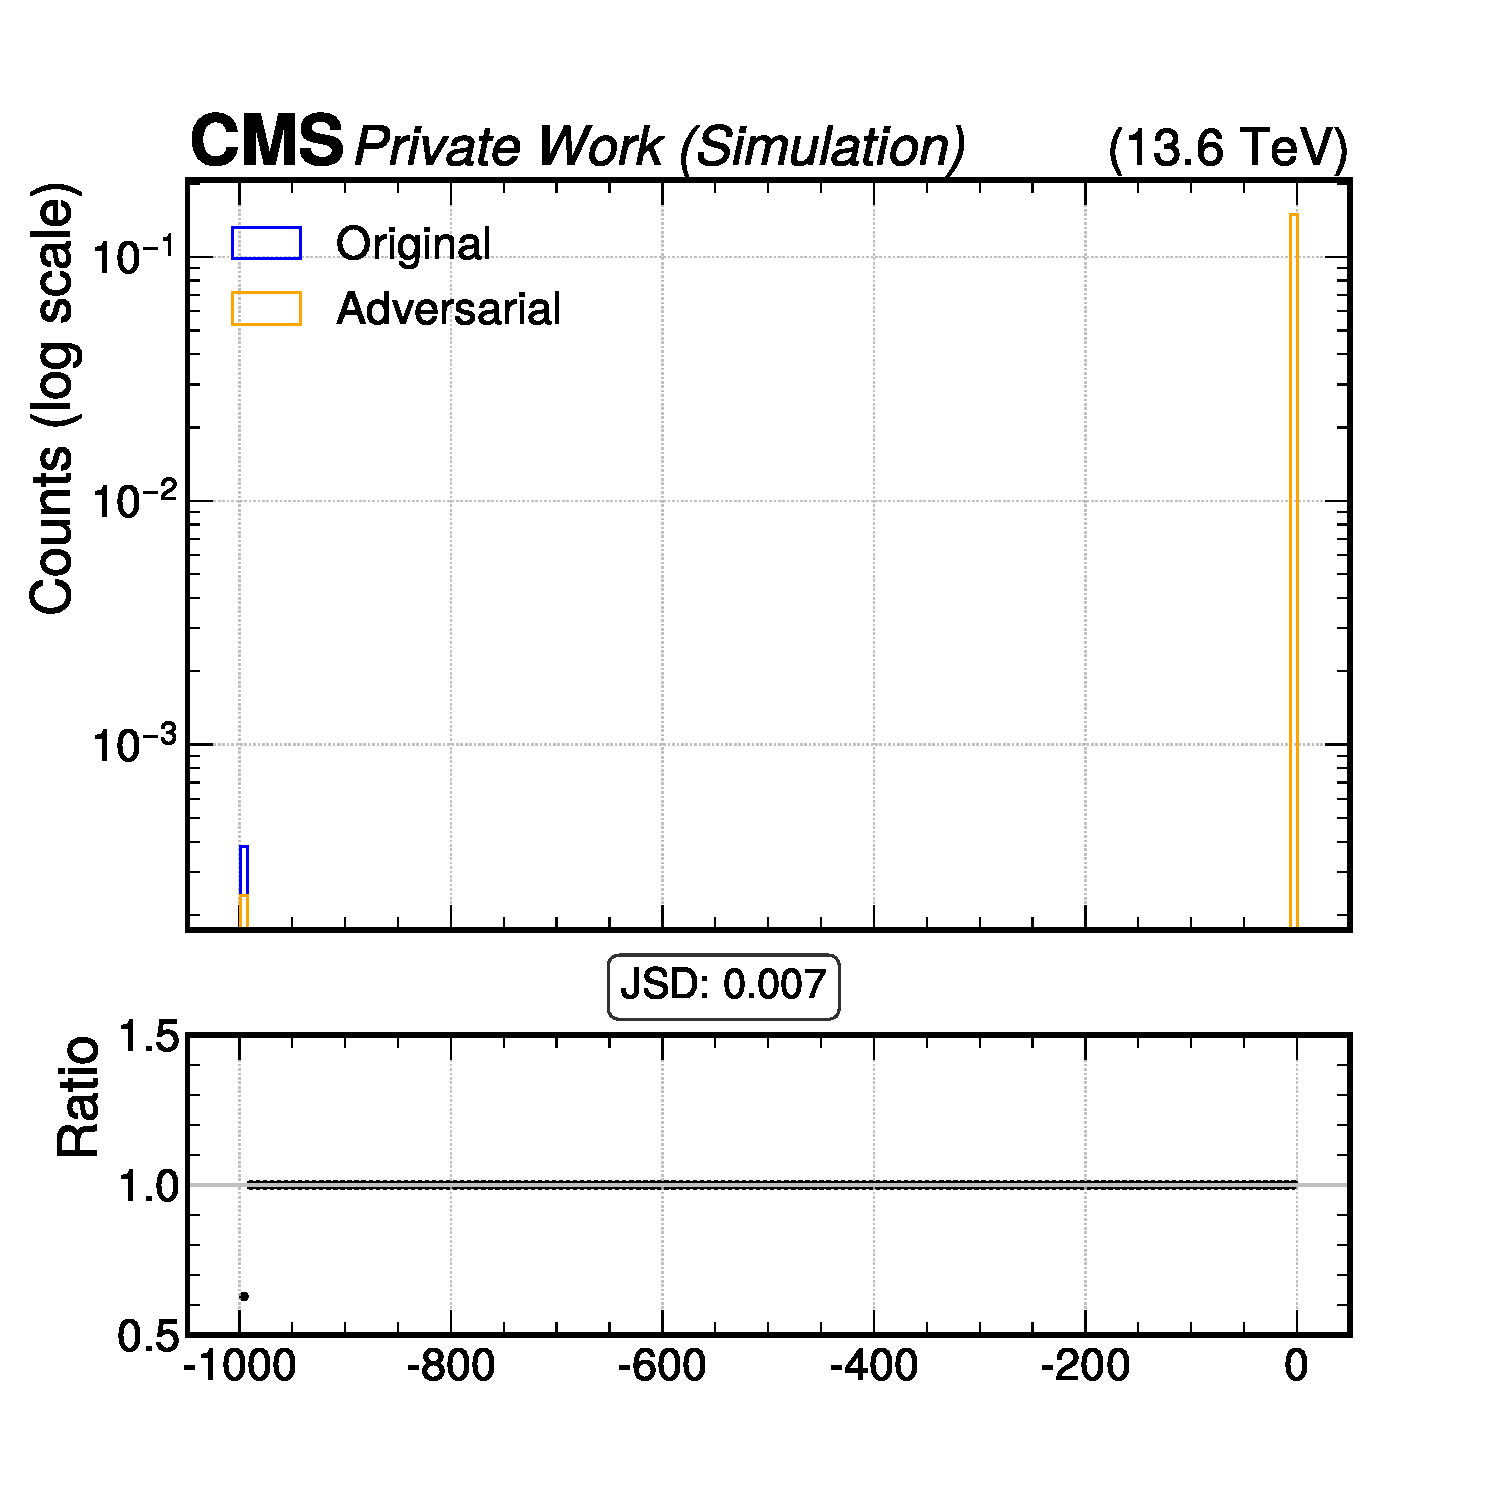
\includegraphics[width=\linewidth]{media/output/features/compare/combined_it_2/cmp_global_features_TagVarCSV_trackSip2dValAboveCharm.pdf}
    \caption*{Input similarity for PIP-PGD(2).}
  \end{subfigure}\hfill
  \begin{subfigure}[t]{0.32\textwidth}
    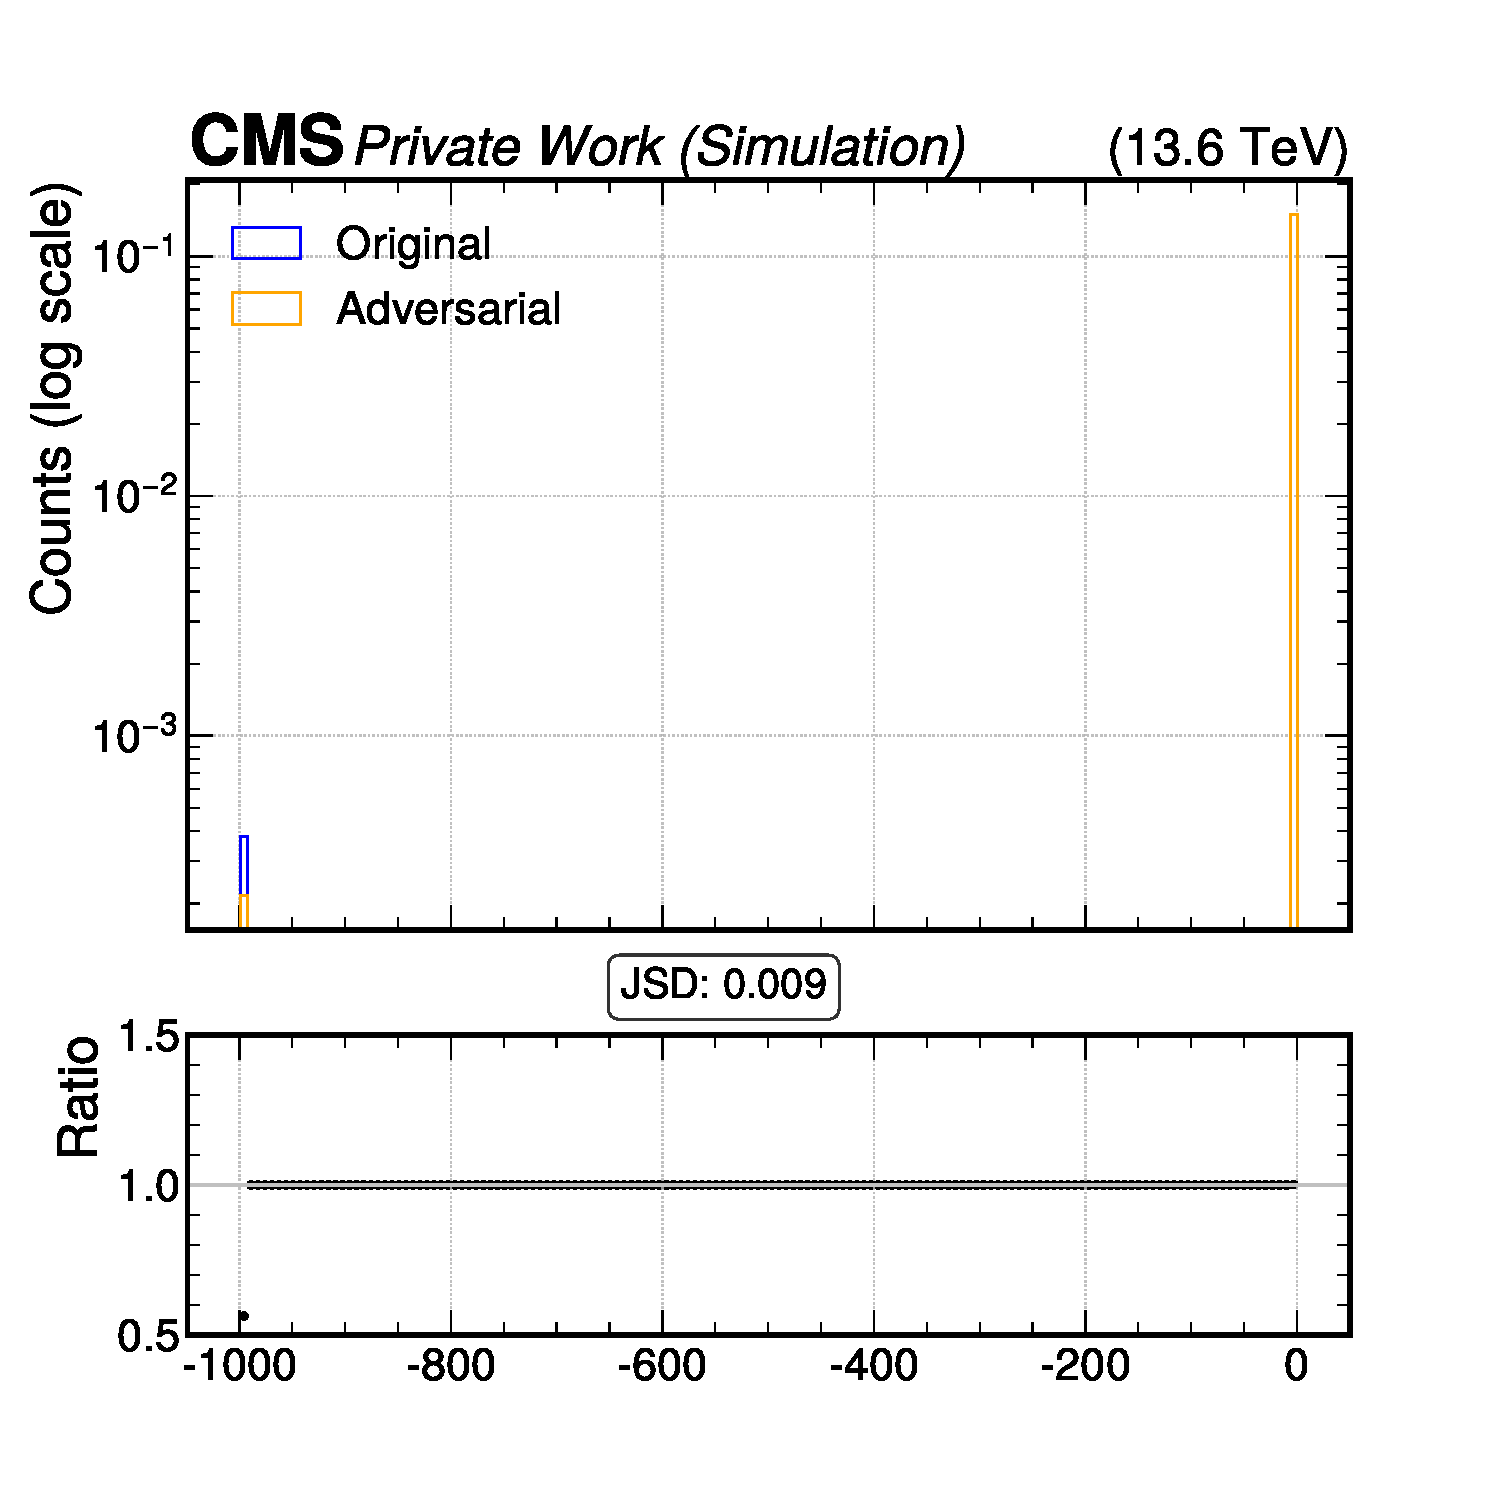
\includegraphics[width=\linewidth]{media/output/features/compare/combined_it_3/cmp_global_features_TagVarCSV_trackSip2dValAboveCharm.pdf}
    \caption*{Input similarity for PIP-PGD(3).}
  \end{subfigure}

  \caption*{Histogram of \texttt{TagVarCSV\_trackSip2dValAboveCharm} for multiple iterations of PIP-PGD tested against nominal inputs.}
  \label{fig:combined_input_TagVarCSV_trackSip2dValAboveCharm}
\end{figure}

\begin{figure}[h]
  \centering
  \begin{subfigure}[t]{0.32\textwidth}
    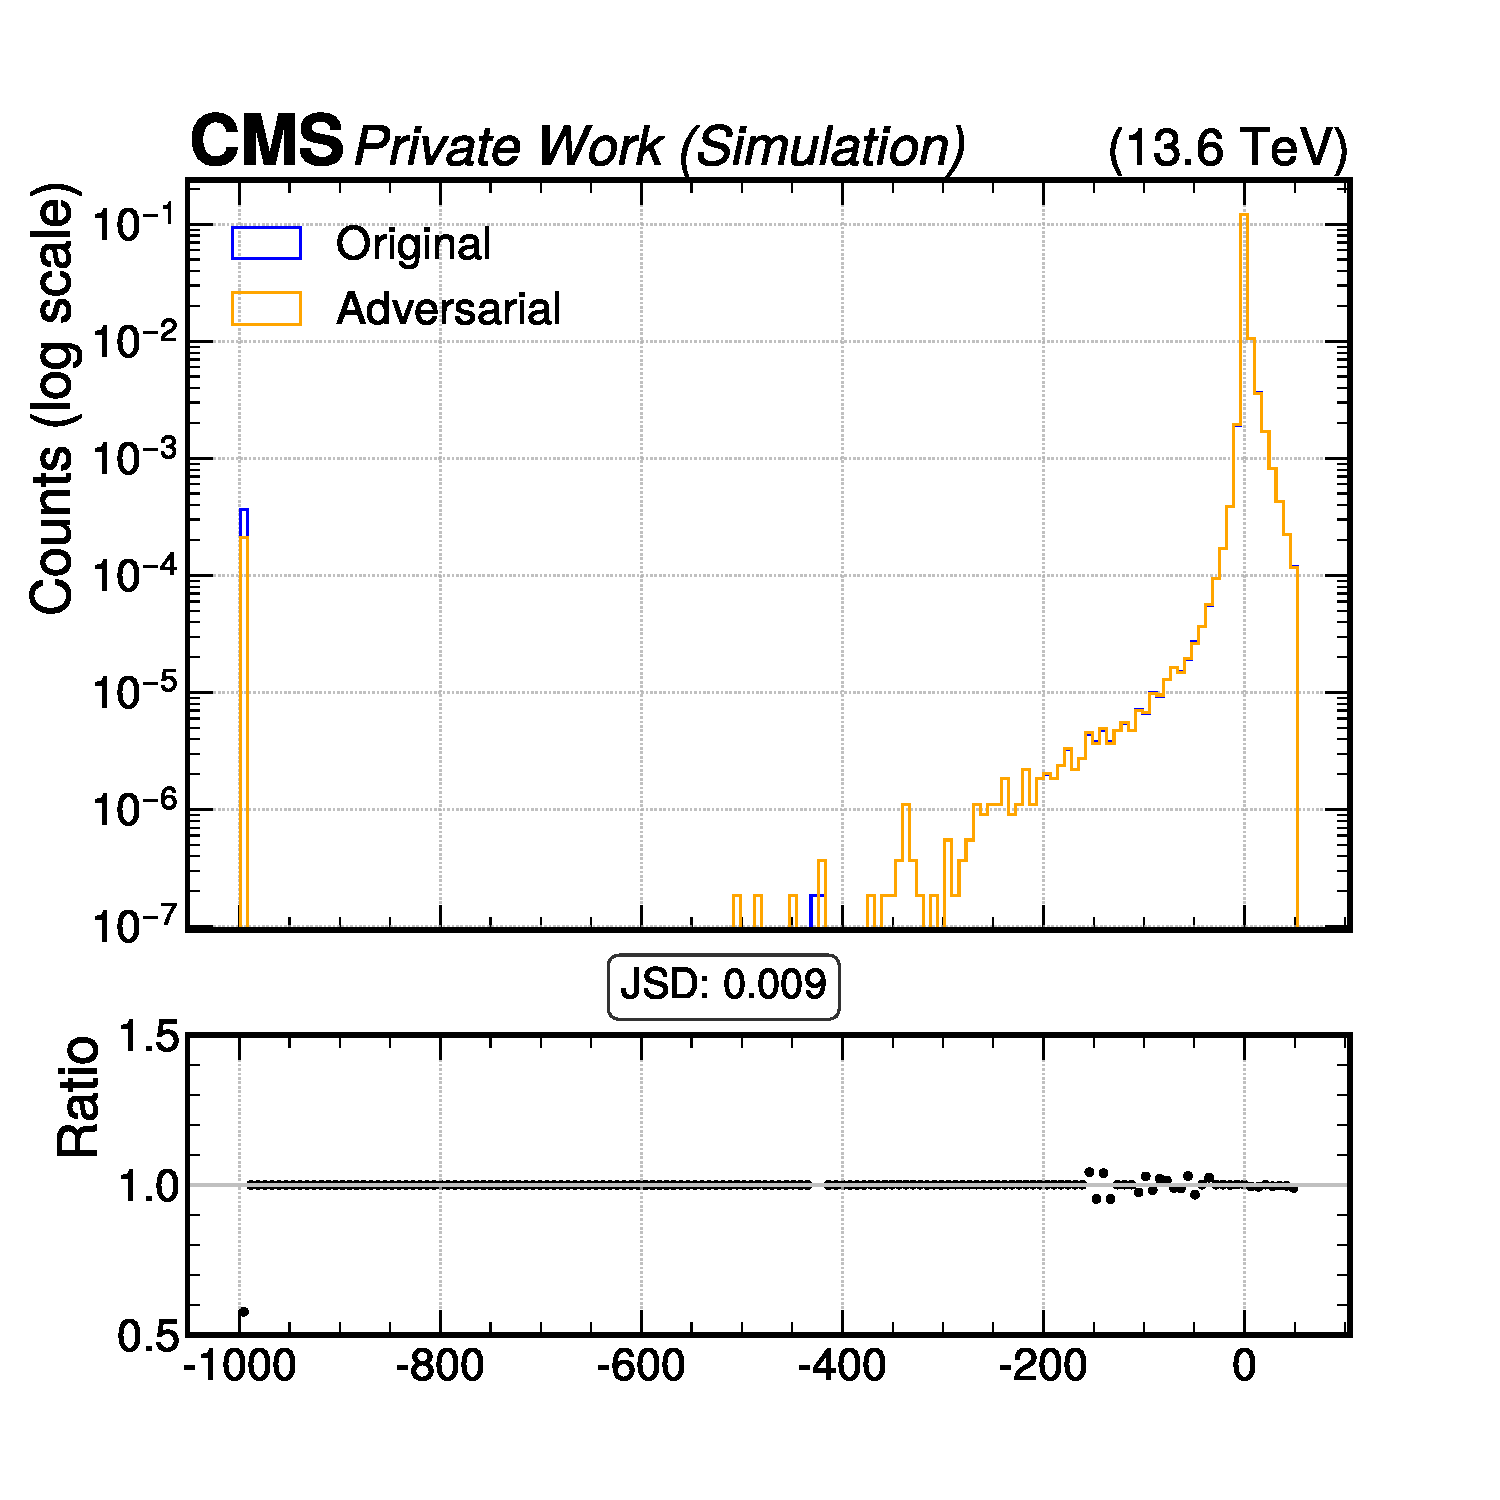
\includegraphics[width=\linewidth]{media/output/features/compare/combined_it_1/cmp_global_features_TagVarCSV_trackSip3dSigAboveCharm.pdf}
    \caption*{Input similarity for PIP-PGD(1).}
  \end{subfigure}\hfill
  \begin{subfigure}[t]{0.32\textwidth}
    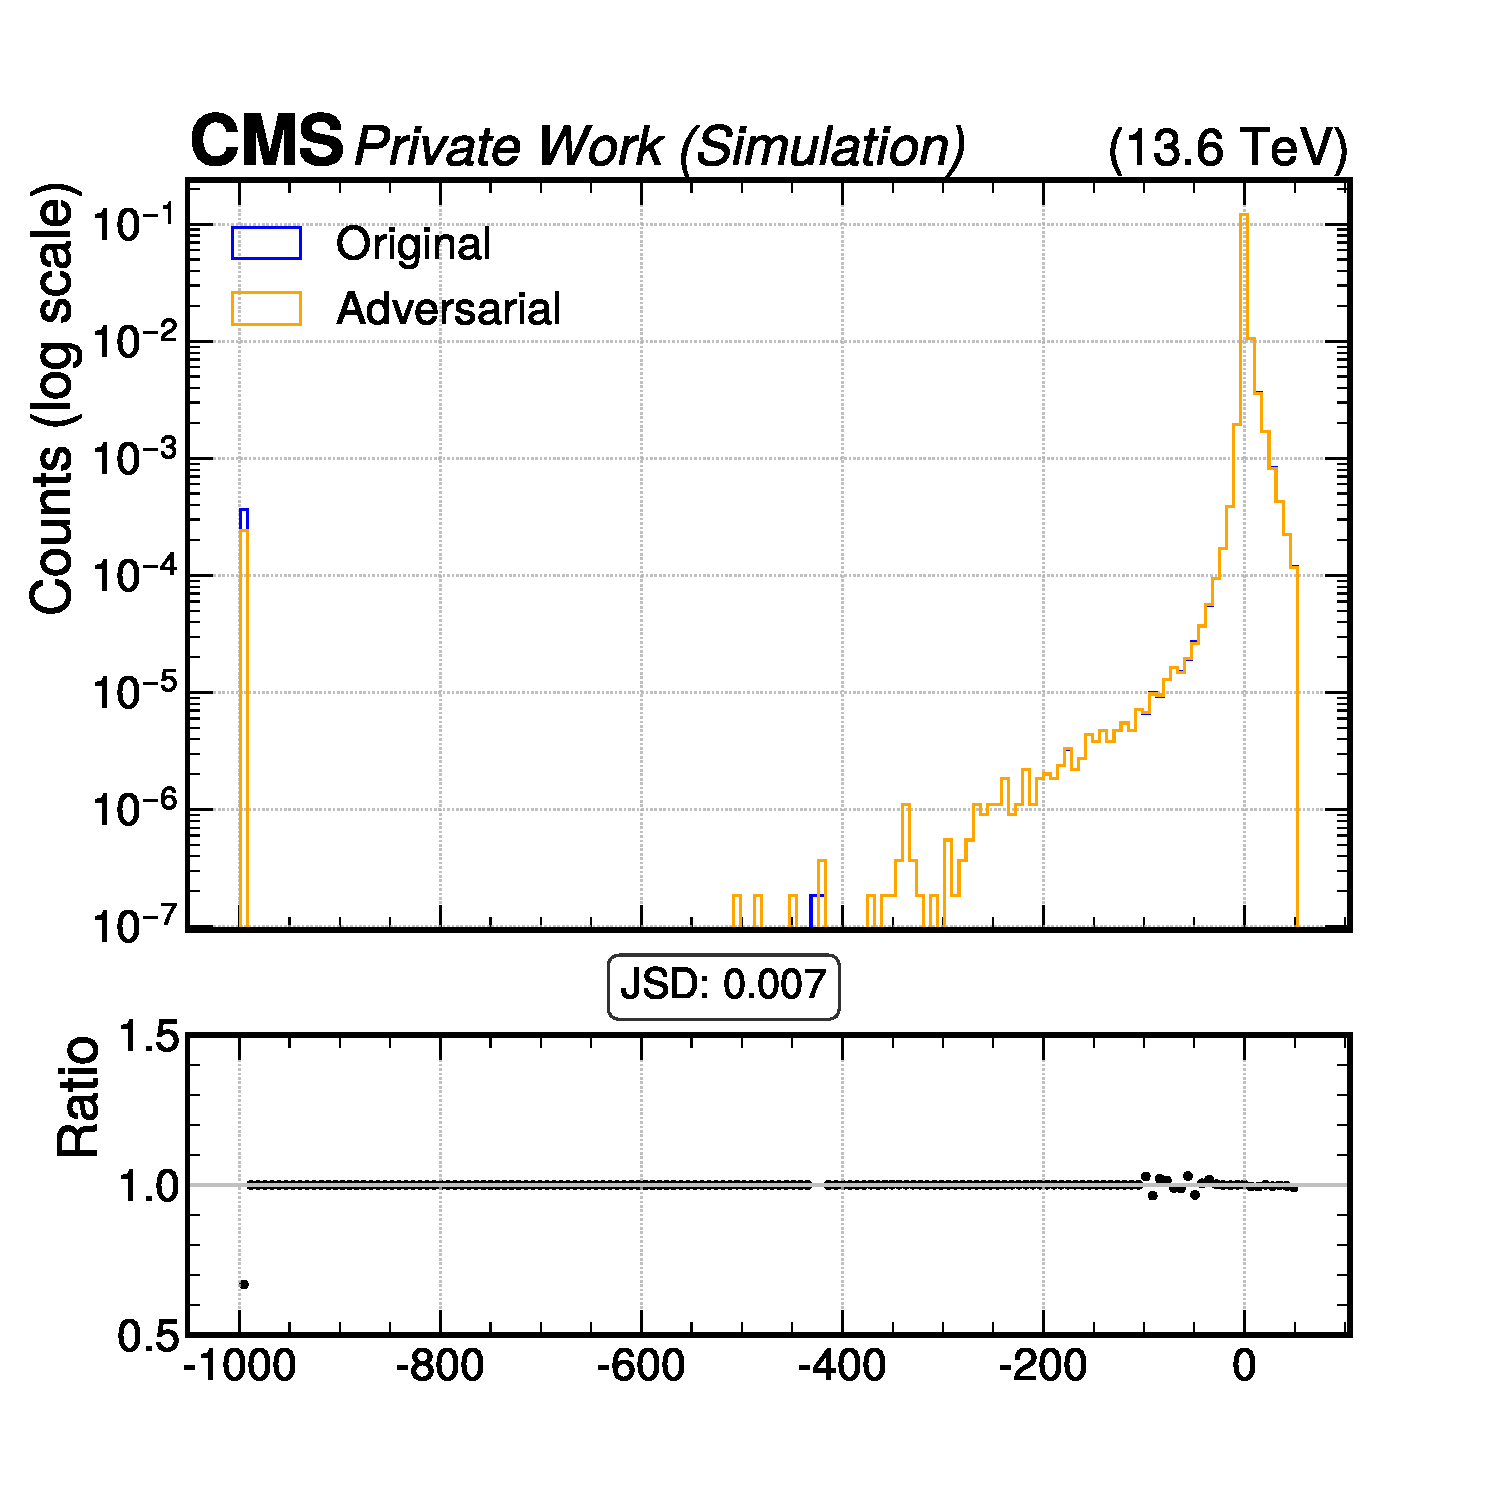
\includegraphics[width=\linewidth]{media/output/features/compare/combined_it_2/cmp_global_features_TagVarCSV_trackSip3dSigAboveCharm.pdf}
    \caption*{Input similarity for PIP-PGD(2).}
  \end{subfigure}\hfill
  \begin{subfigure}[t]{0.32\textwidth}
    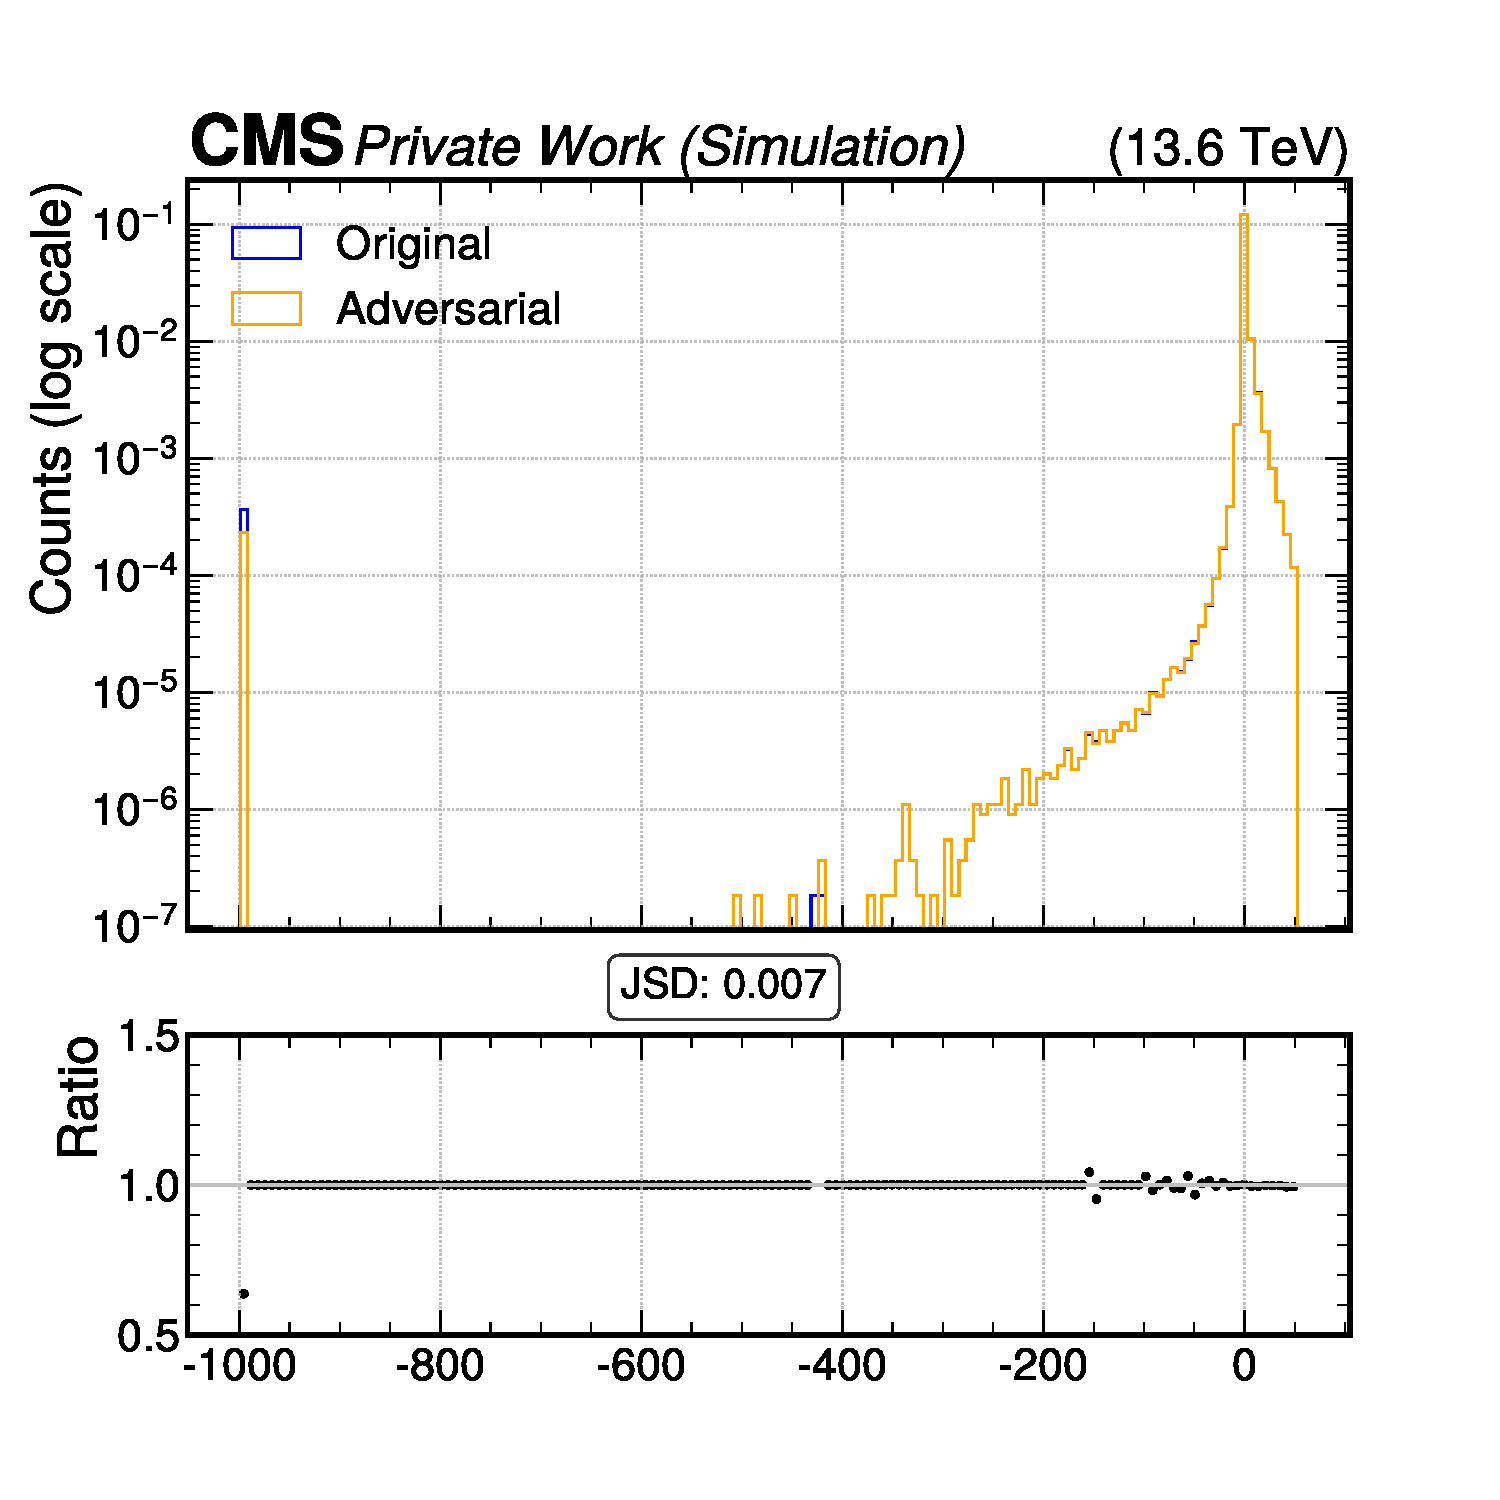
\includegraphics[width=\linewidth]{media/output/features/compare/combined_it_3/cmp_global_features_TagVarCSV_trackSip3dSigAboveCharm.pdf}
    \caption*{Input similarity for PIP-PGD(3).}
  \end{subfigure}

  \caption*{Histogram of \texttt{TagVarCSV\_trackSip3dSigAboveCharm} for multiple iterations of PIP-PGD tested against nominal inputs.}
  \label{fig:combined_input_TagVarCSV_trackSip3dSigAboveCharm}
\end{figure}

\begin{figure}[h]
  \centering
  \begin{subfigure}[t]{0.32\textwidth}
    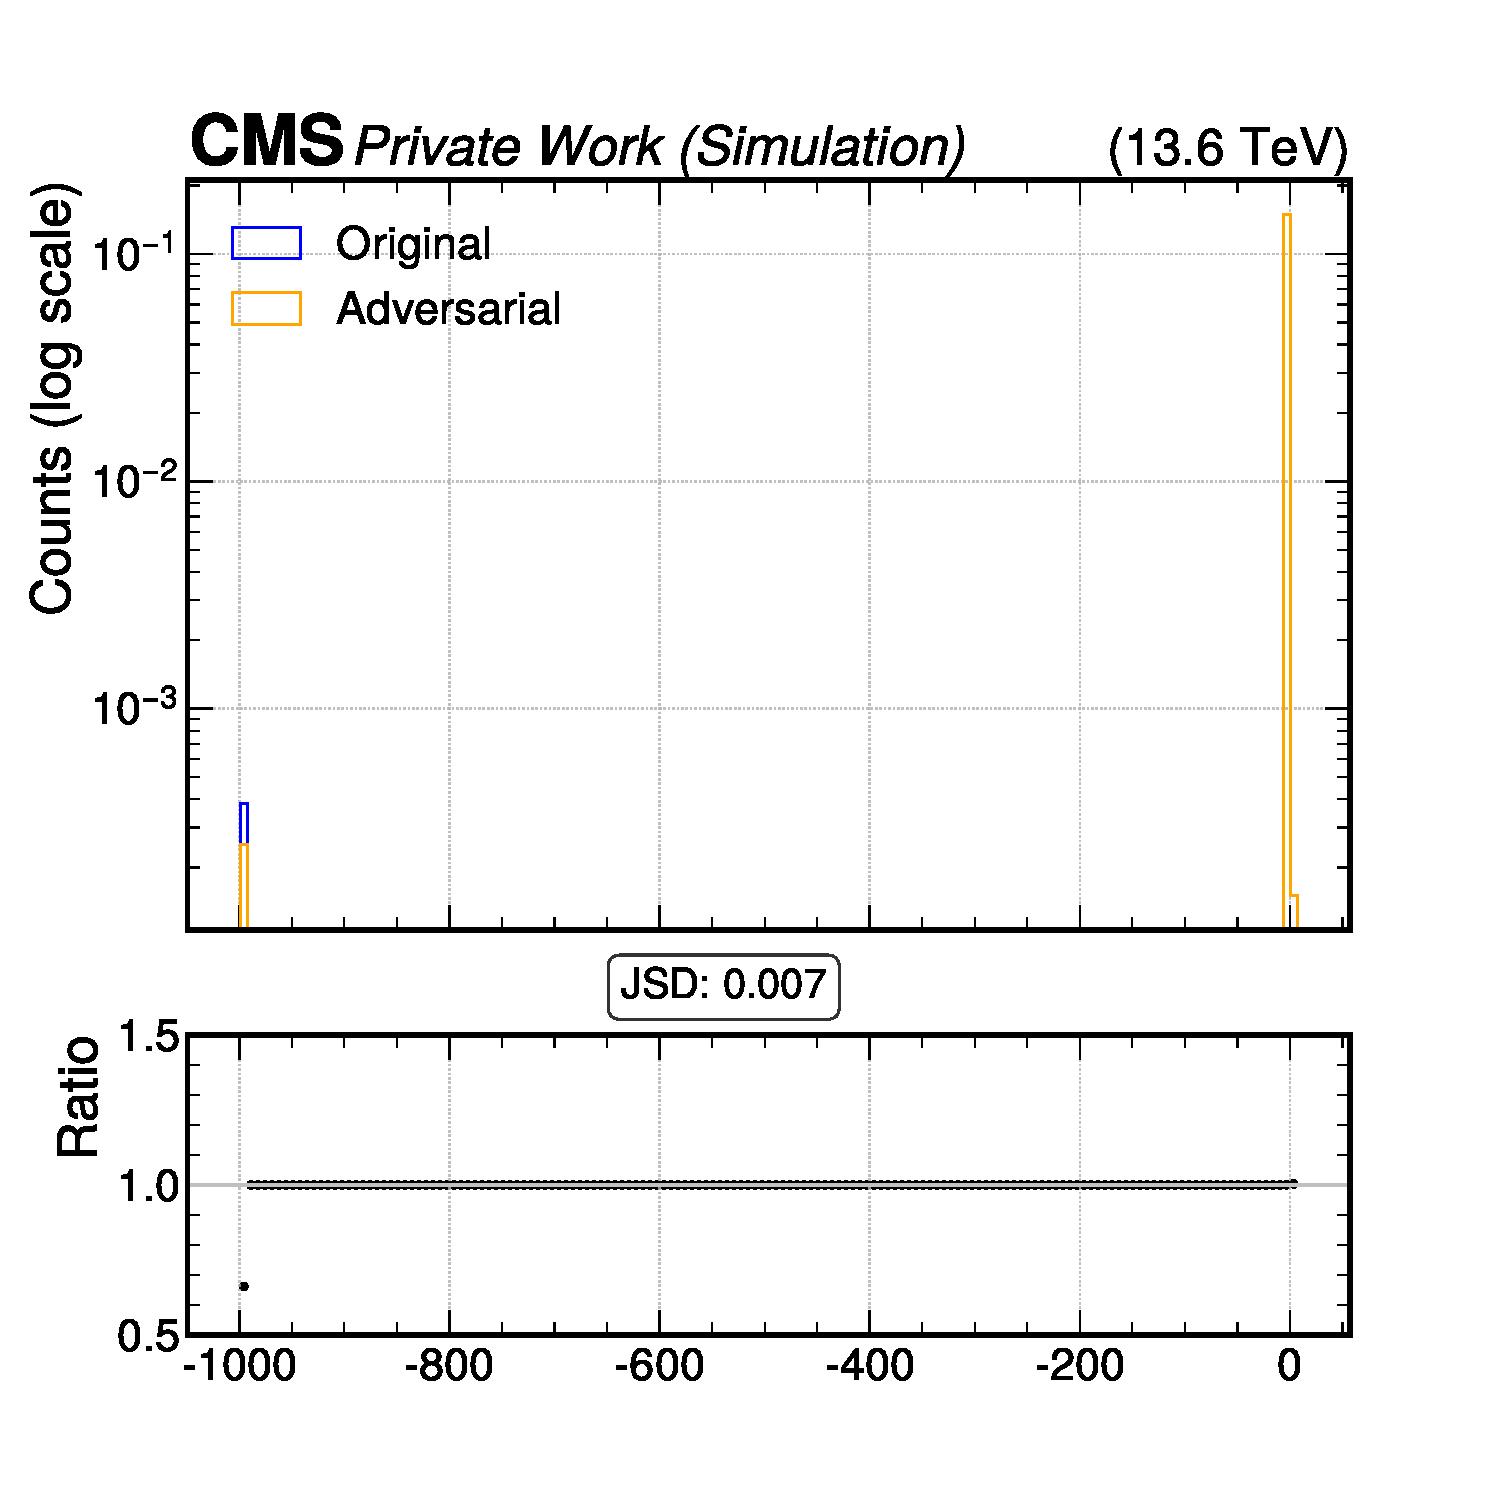
\includegraphics[width=\linewidth]{media/output/features/compare/combined_it_1/cmp_global_features_TagVarCSV_trackSip3dValAboveCharm.pdf}
    \caption*{Input similarity for PIP-PGD(1).}
  \end{subfigure}\hfill
  \begin{subfigure}[t]{0.32\textwidth}
    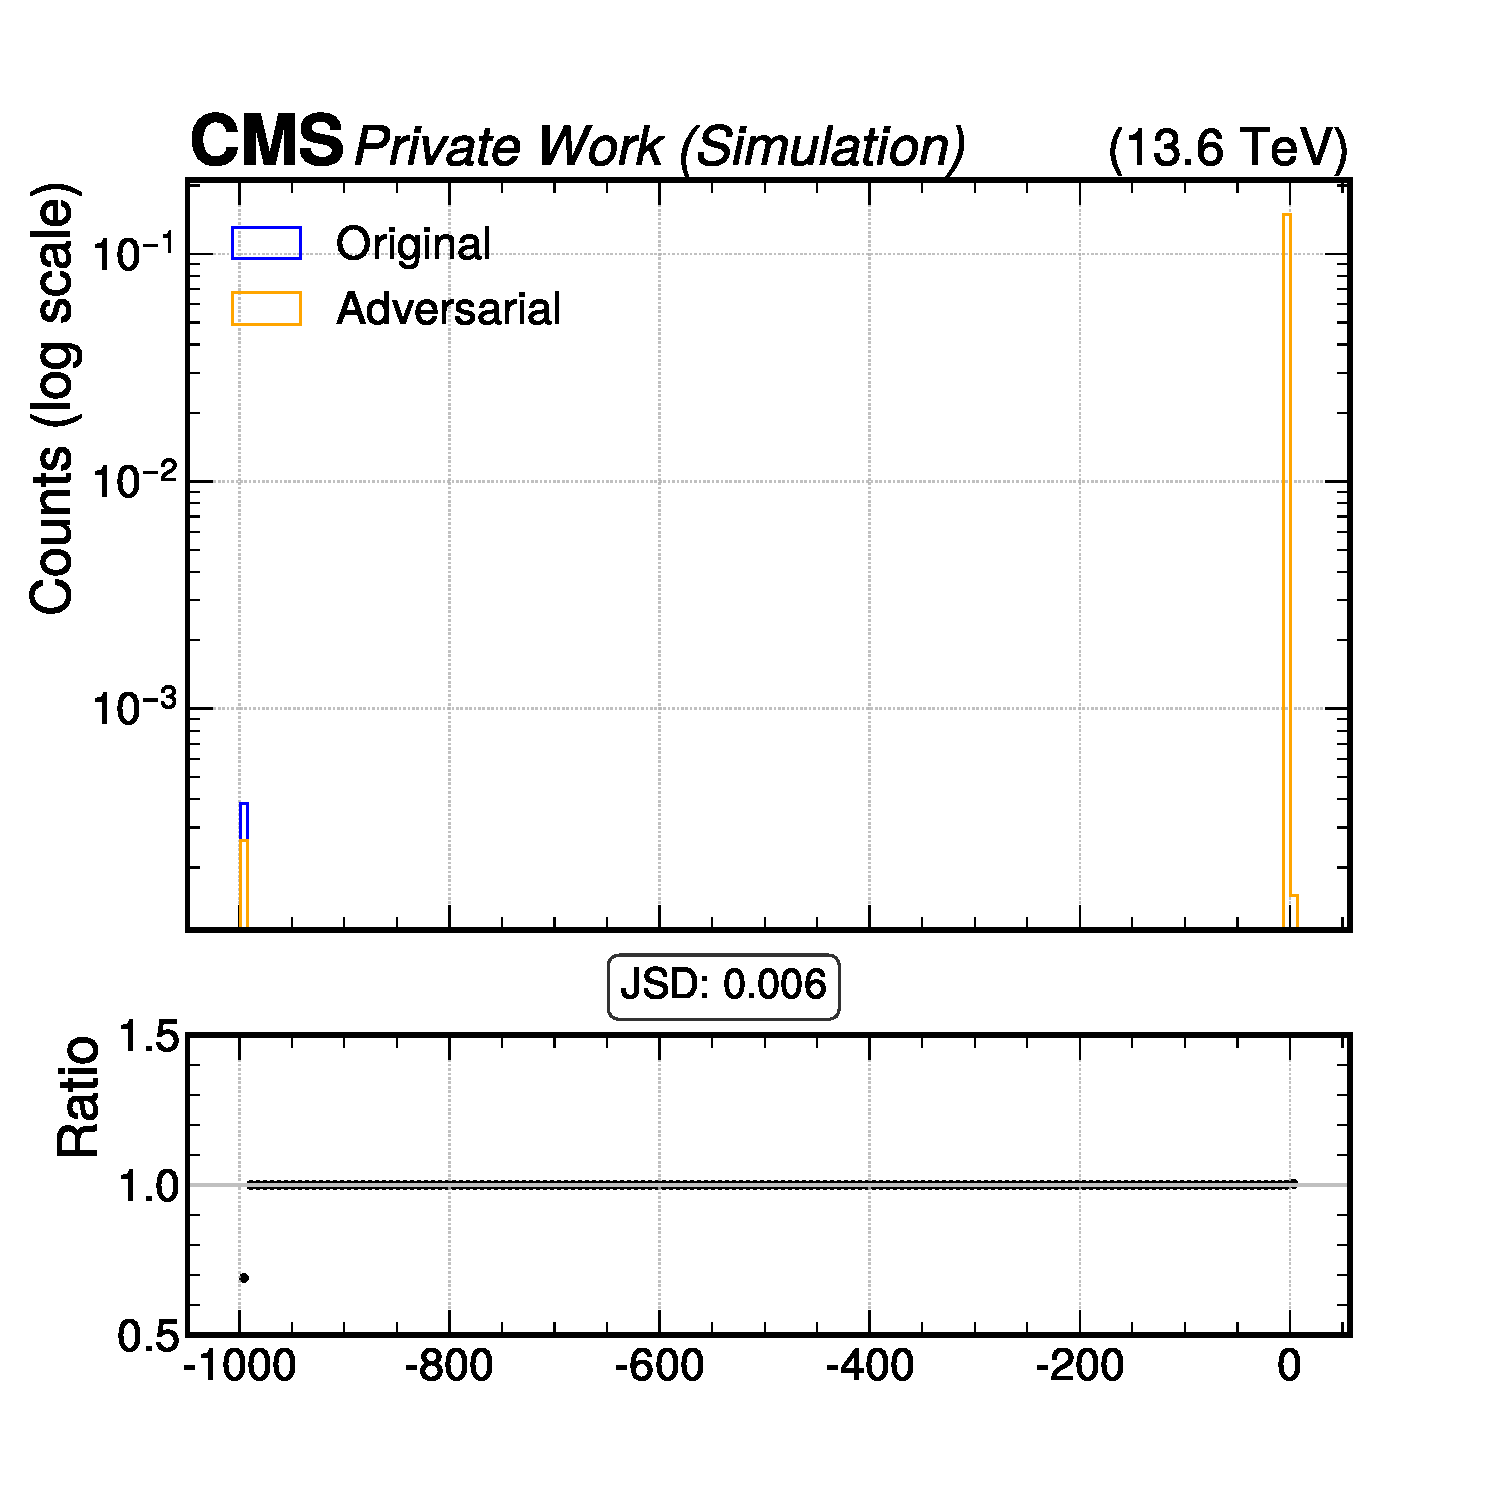
\includegraphics[width=\linewidth]{media/output/features/compare/combined_it_2/cmp_global_features_TagVarCSV_trackSip3dValAboveCharm.pdf}
    \caption*{Input similarity for PIP-PGD(2).}
  \end{subfigure}\hfill
  \begin{subfigure}[t]{0.32\textwidth}
    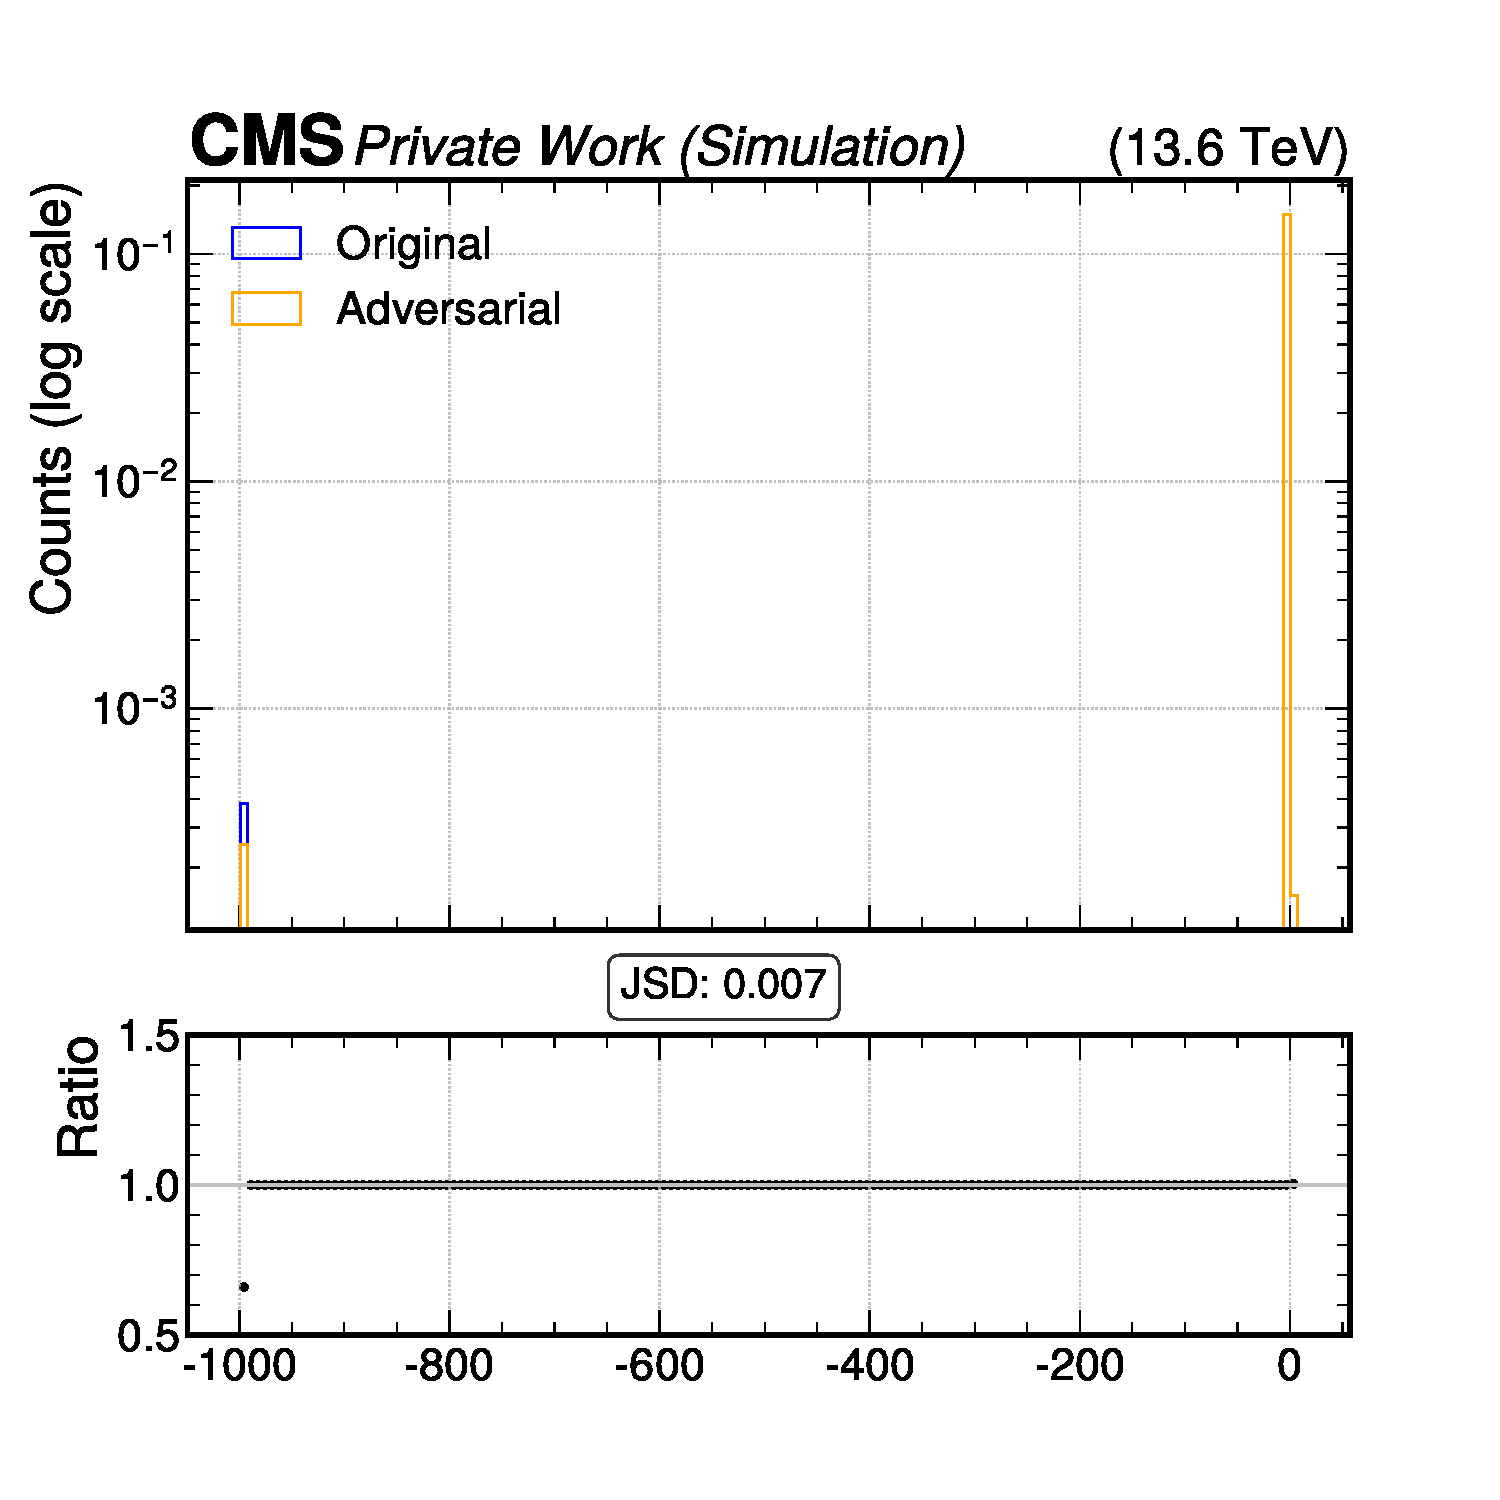
\includegraphics[width=\linewidth]{media/output/features/compare/combined_it_3/cmp_global_features_TagVarCSV_trackSip3dValAboveCharm.pdf}
    \caption*{Input similarity for PIP-PGD(3).}
  \end{subfigure}

  \caption*{Histogram of \texttt{TagVarCSV\_trackSip3dValAboveCharm} for multiple iterations of PIP-PGD tested against nominal inputs.}
  \label{fig:combined_input_TagVarCSV_trackSip3dValAboveCharm}
\end{figure}

\begin{figure}[h]
  \centering
  \begin{subfigure}[t]{0.32\textwidth}
    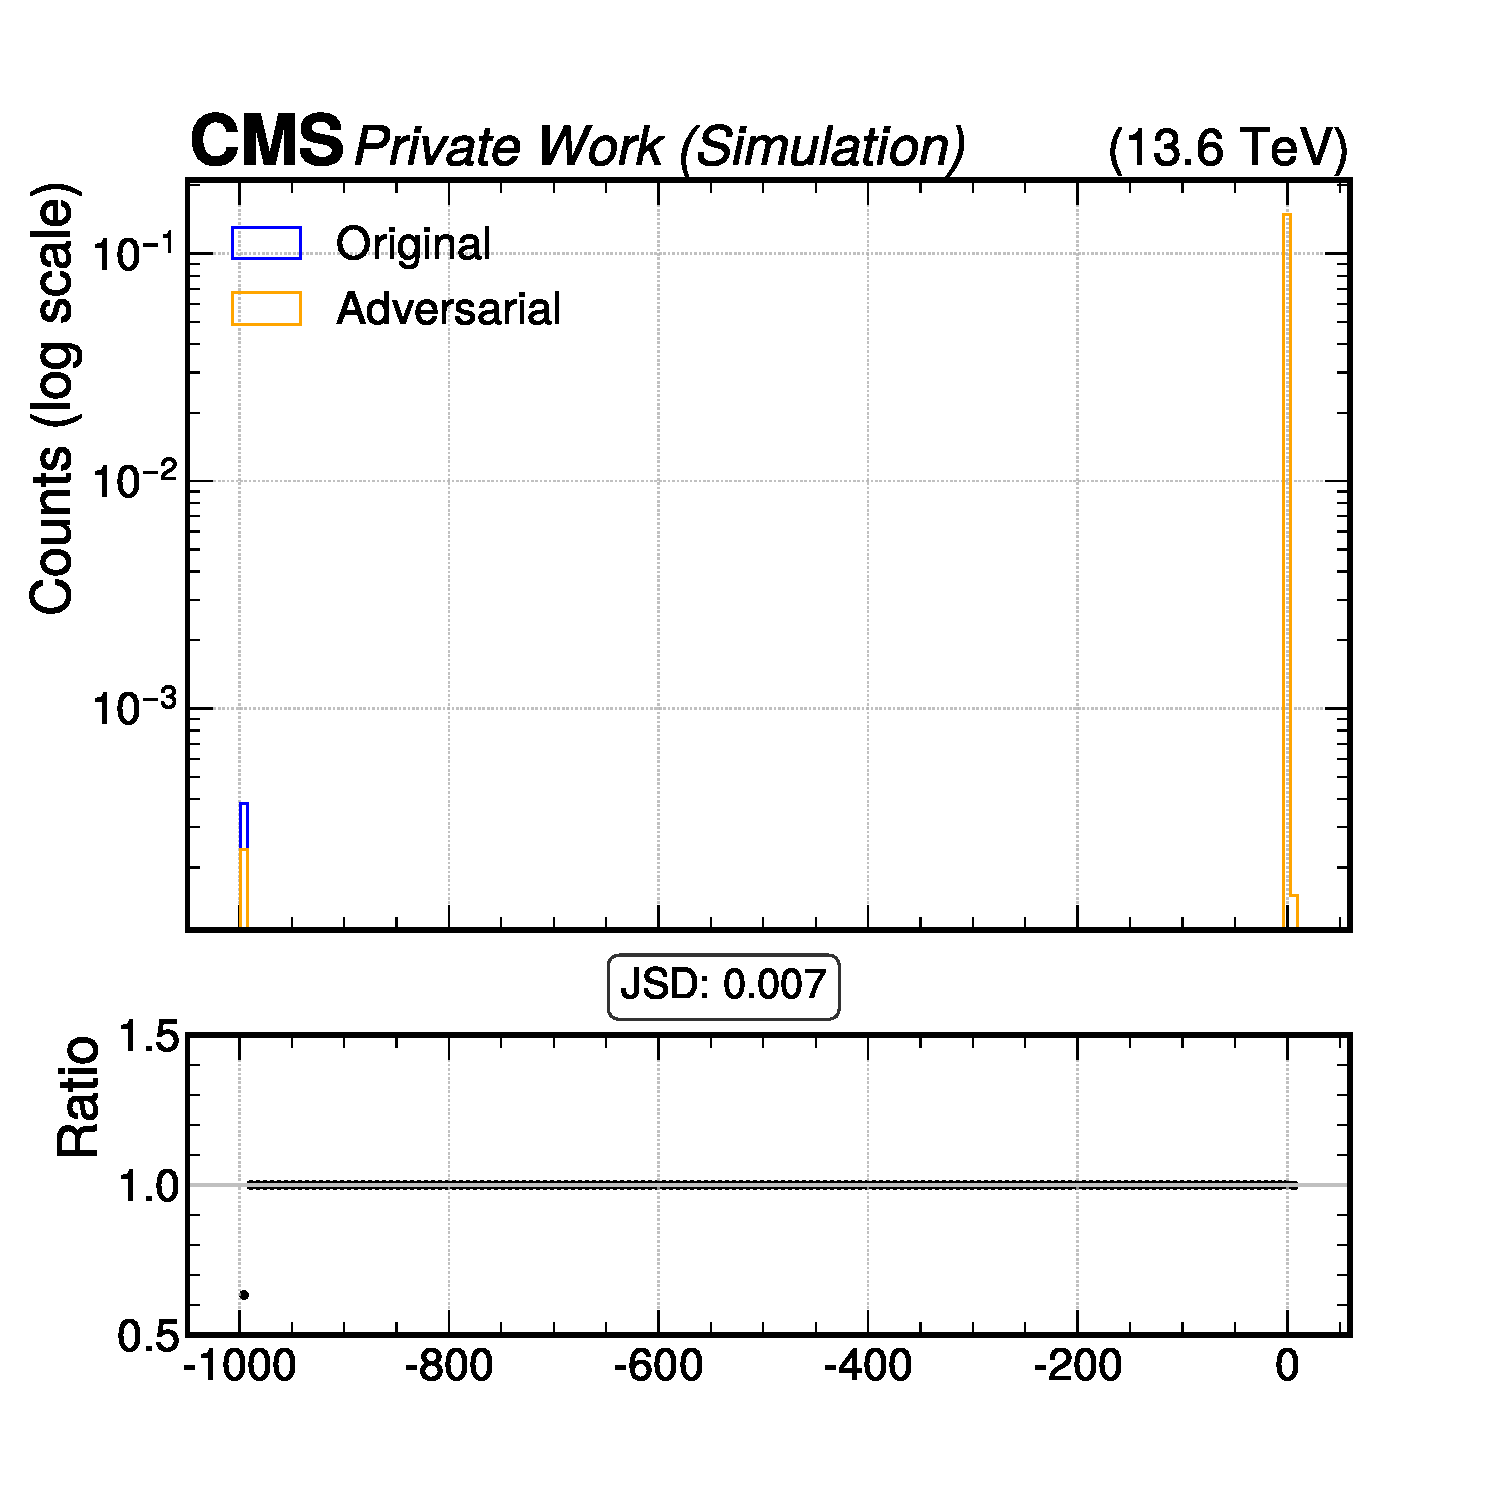
\includegraphics[width=\linewidth]{media/output/features/compare/combined_it_1/cmp_global_features_TagVarCSV_trackSumJetDeltaR.pdf}
    \caption*{Input similarity for PIP-PGD(1).}
  \end{subfigure}\hfill
  \begin{subfigure}[t]{0.32\textwidth}
    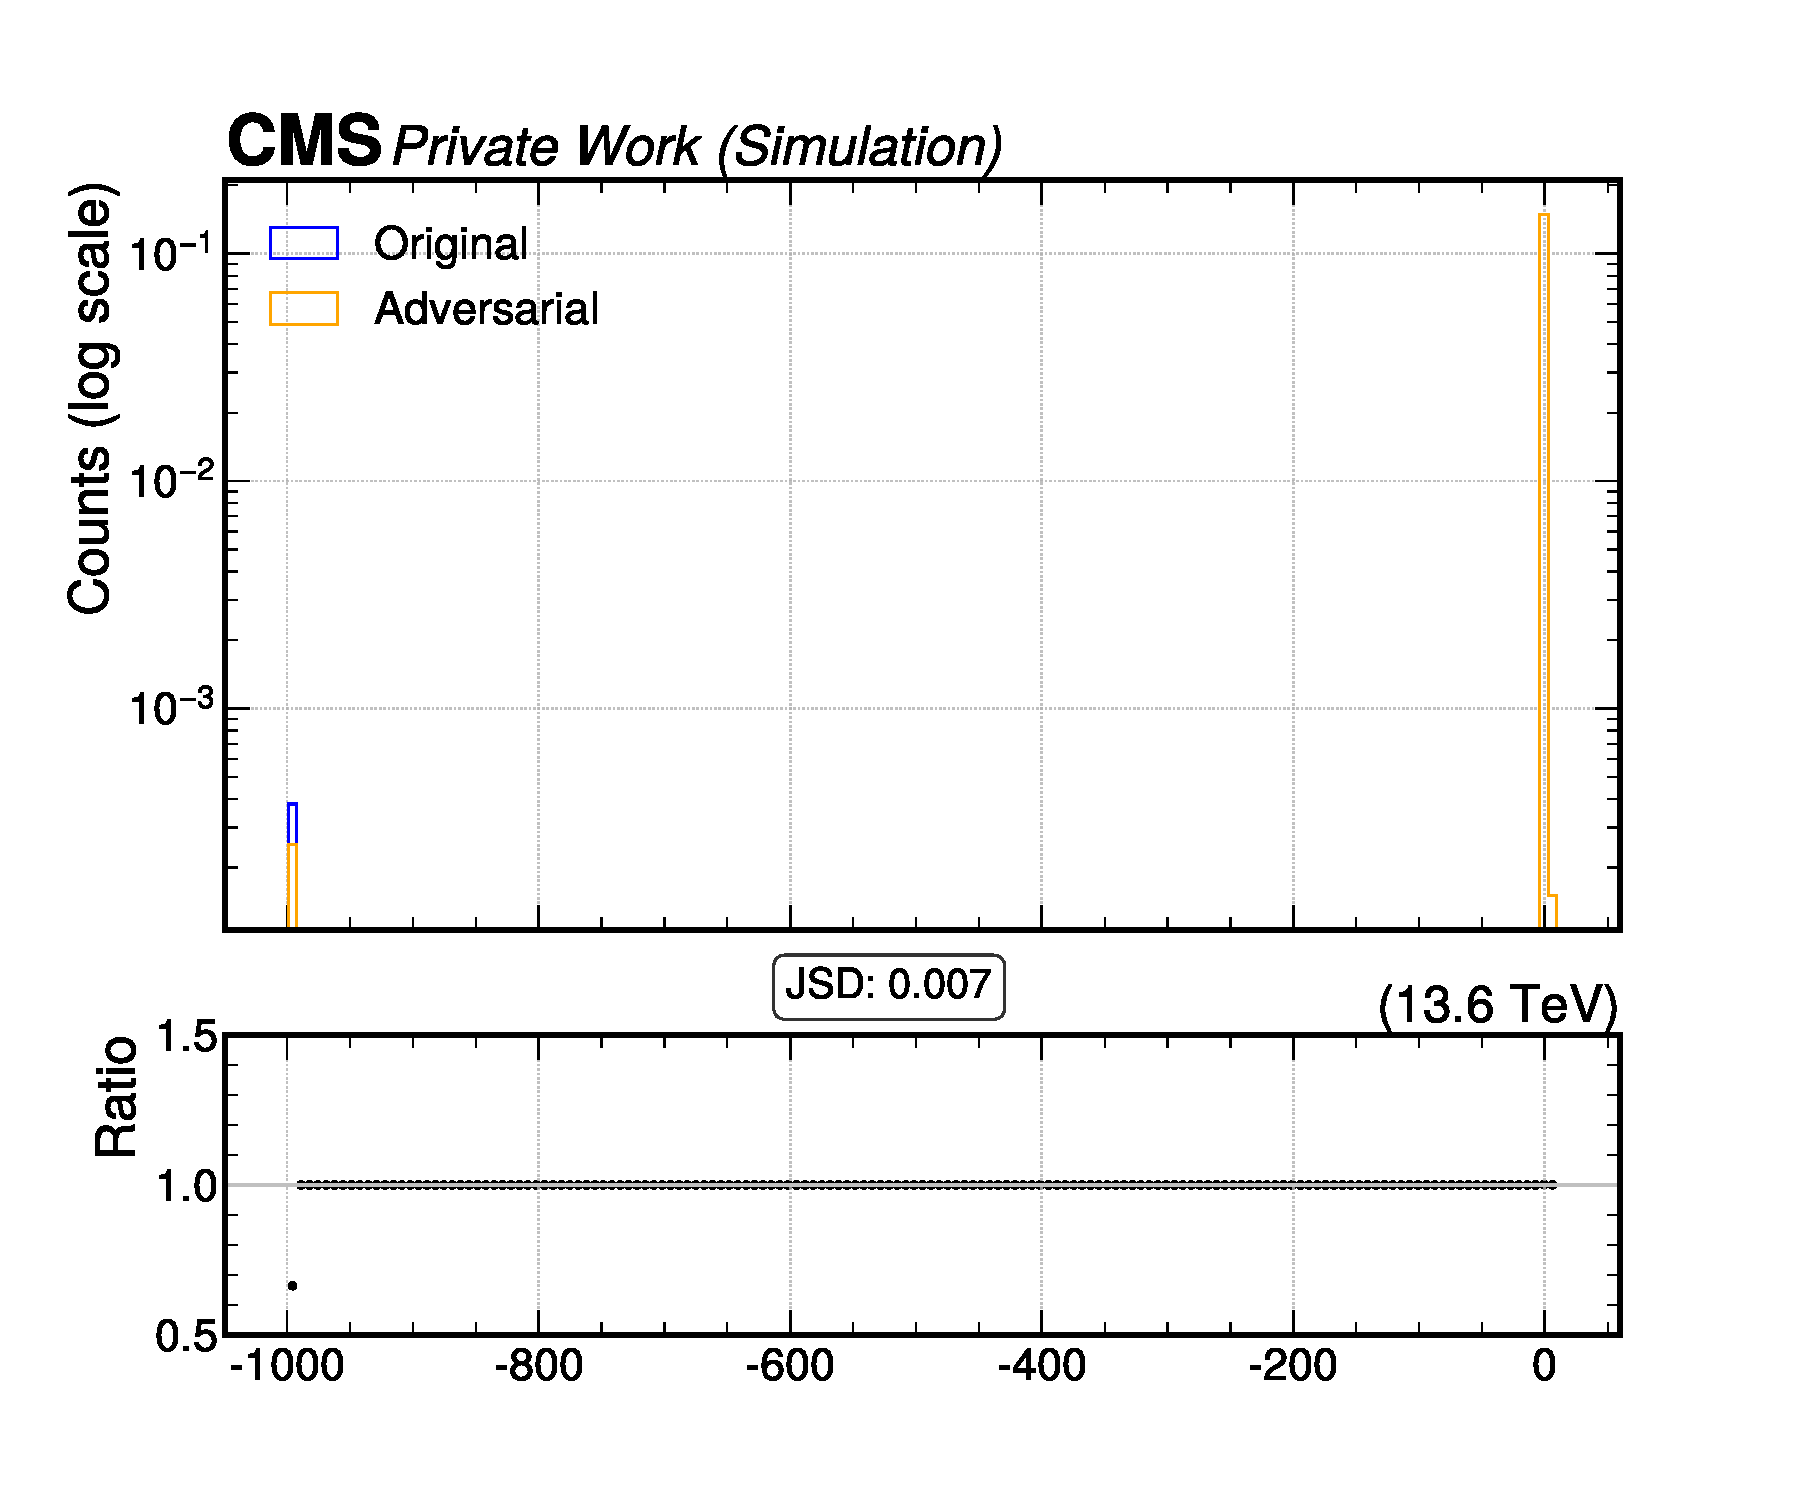
\includegraphics[width=\linewidth]{media/output/features/compare/combined_it_2/cmp_global_features_TagVarCSV_trackSumJetDeltaR.pdf}
    \caption*{Input similarity for PIP-PGD(2).}
  \end{subfigure}\hfill
  \begin{subfigure}[t]{0.32\textwidth}
    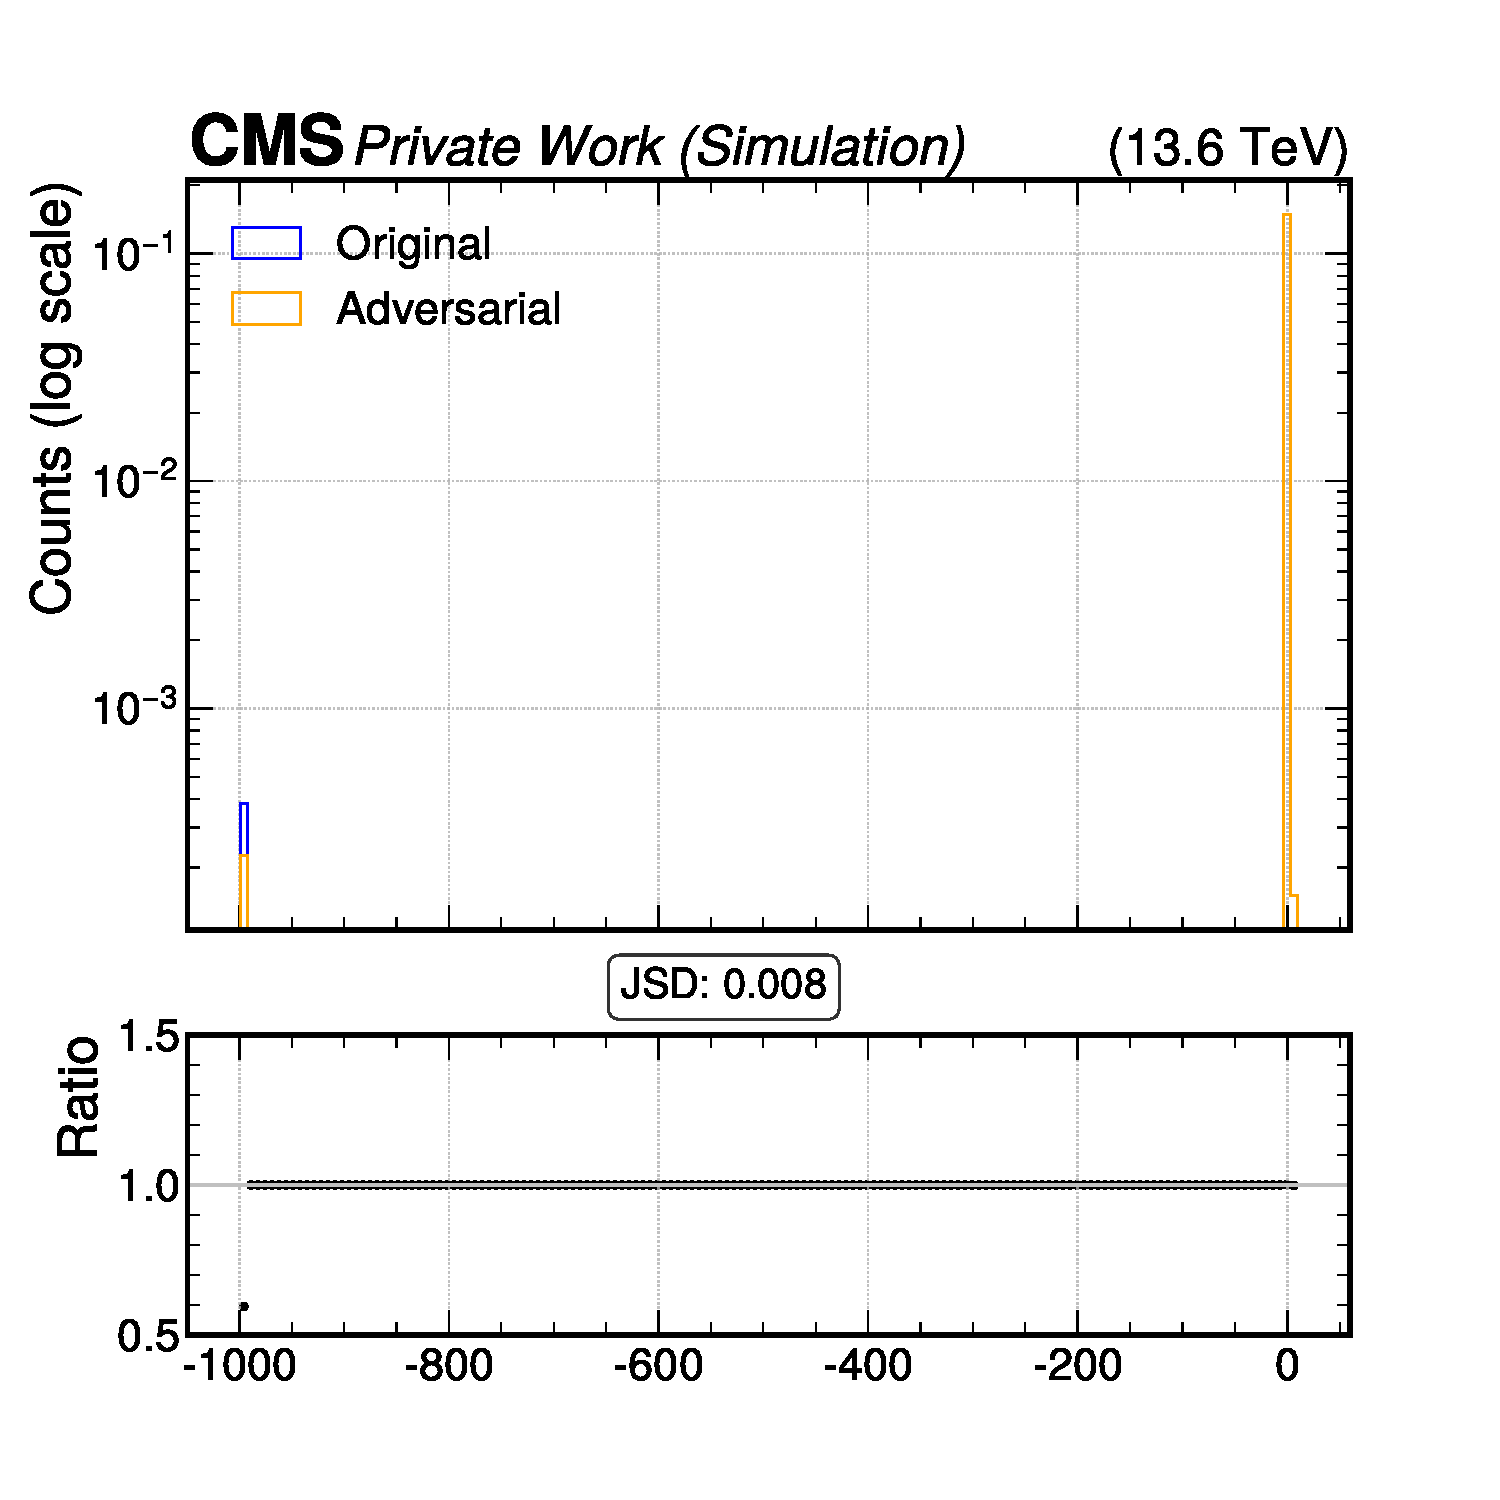
\includegraphics[width=\linewidth]{media/output/features/compare/combined_it_3/cmp_global_features_TagVarCSV_trackSumJetDeltaR.pdf}
    \caption*{Input similarity for PIP-PGD(3).}
  \end{subfigure}

  \caption*{Histogram of \texttt{TagVarCSV\_trackSumJetDeltaR} for multiple iterations of PIP-PGD tested against nominal inputs.}
  \label{fig:combined_input_TagVarCSV_trackSumJetDeltaR}
\end{figure}

\begin{figure}[h]
  \centering
  \begin{subfigure}[t]{0.32\textwidth}
    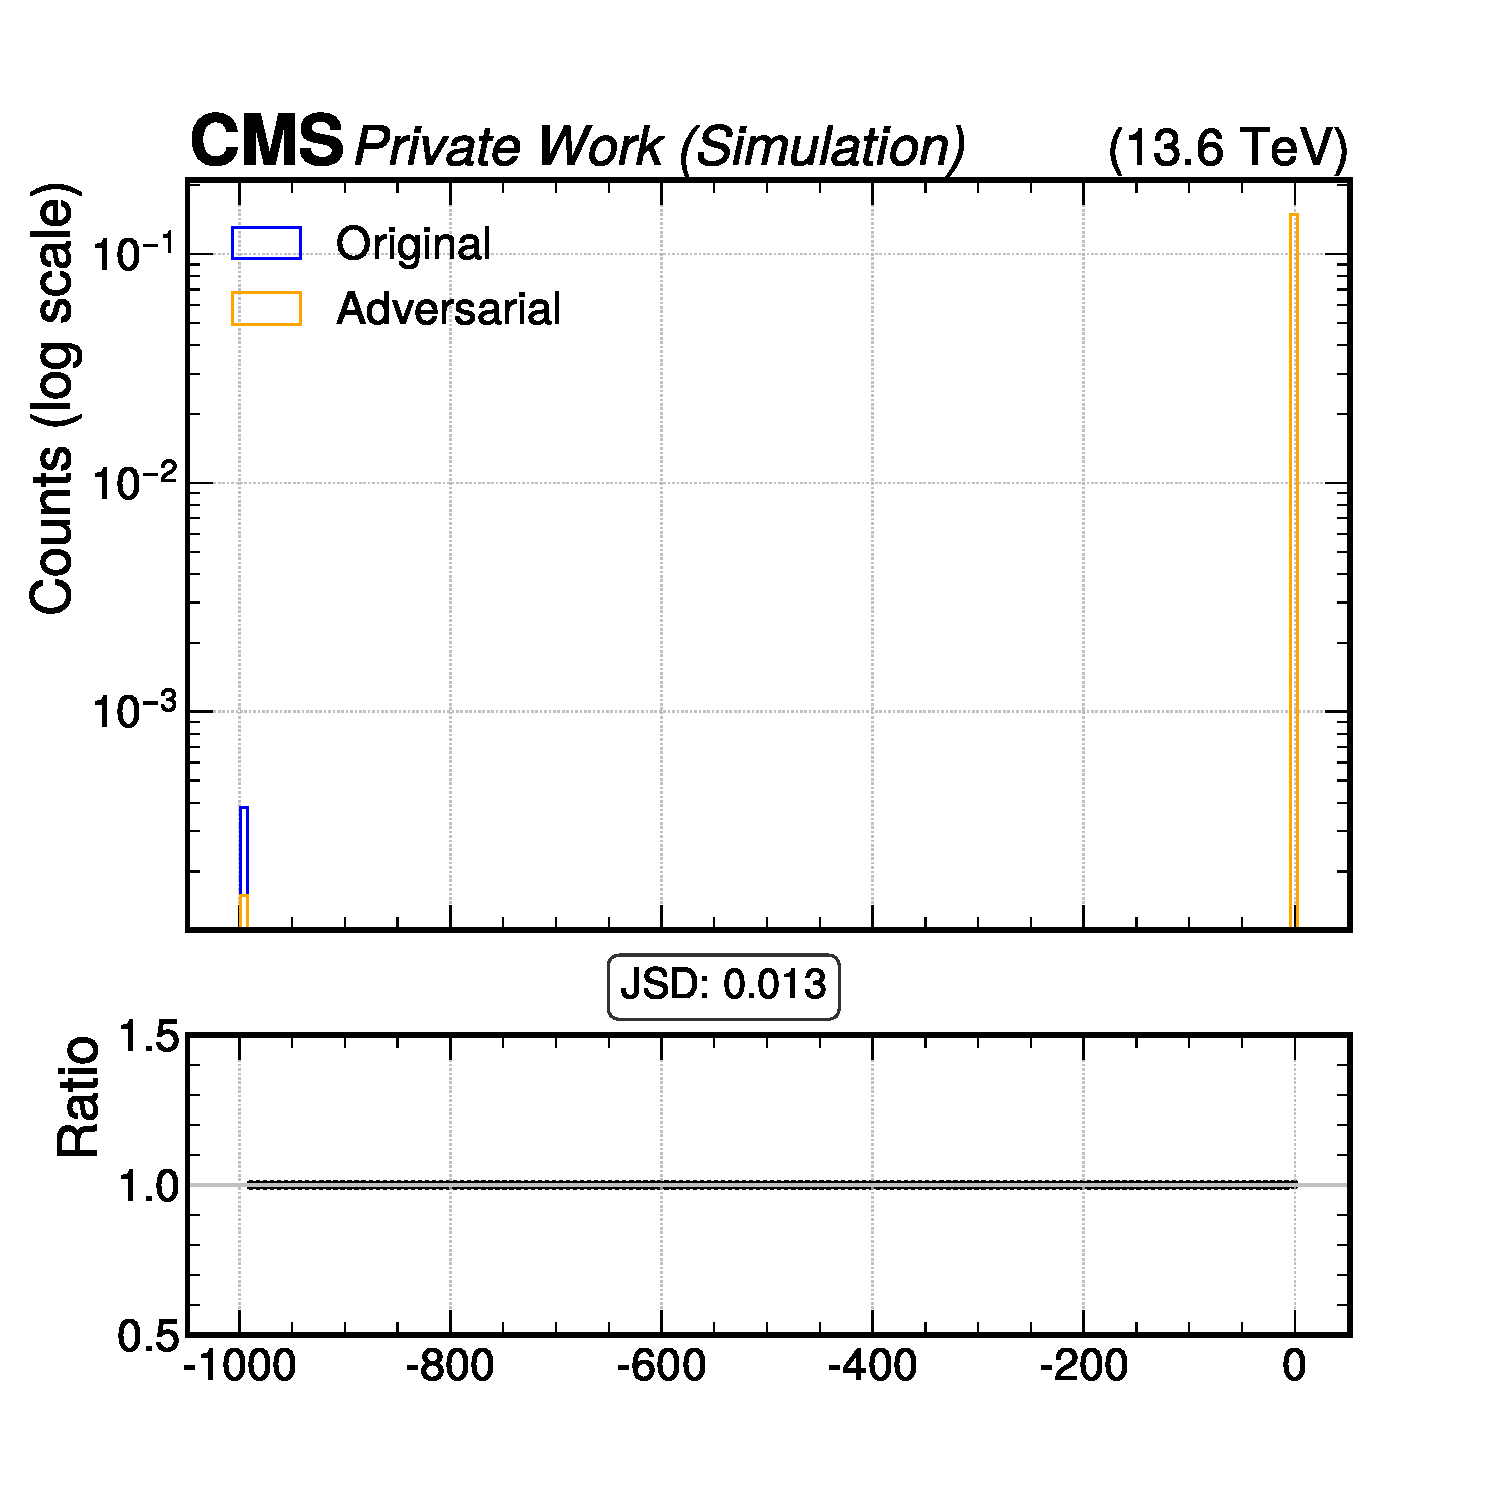
\includegraphics[width=\linewidth]{media/output/features/compare/combined_it_1/cmp_global_features_TagVarCSV_trackSumJetEtRatio.pdf}
    \caption*{Input similarity for PIP-PGD(1).}
  \end{subfigure}\hfill
  \begin{subfigure}[t]{0.32\textwidth}
    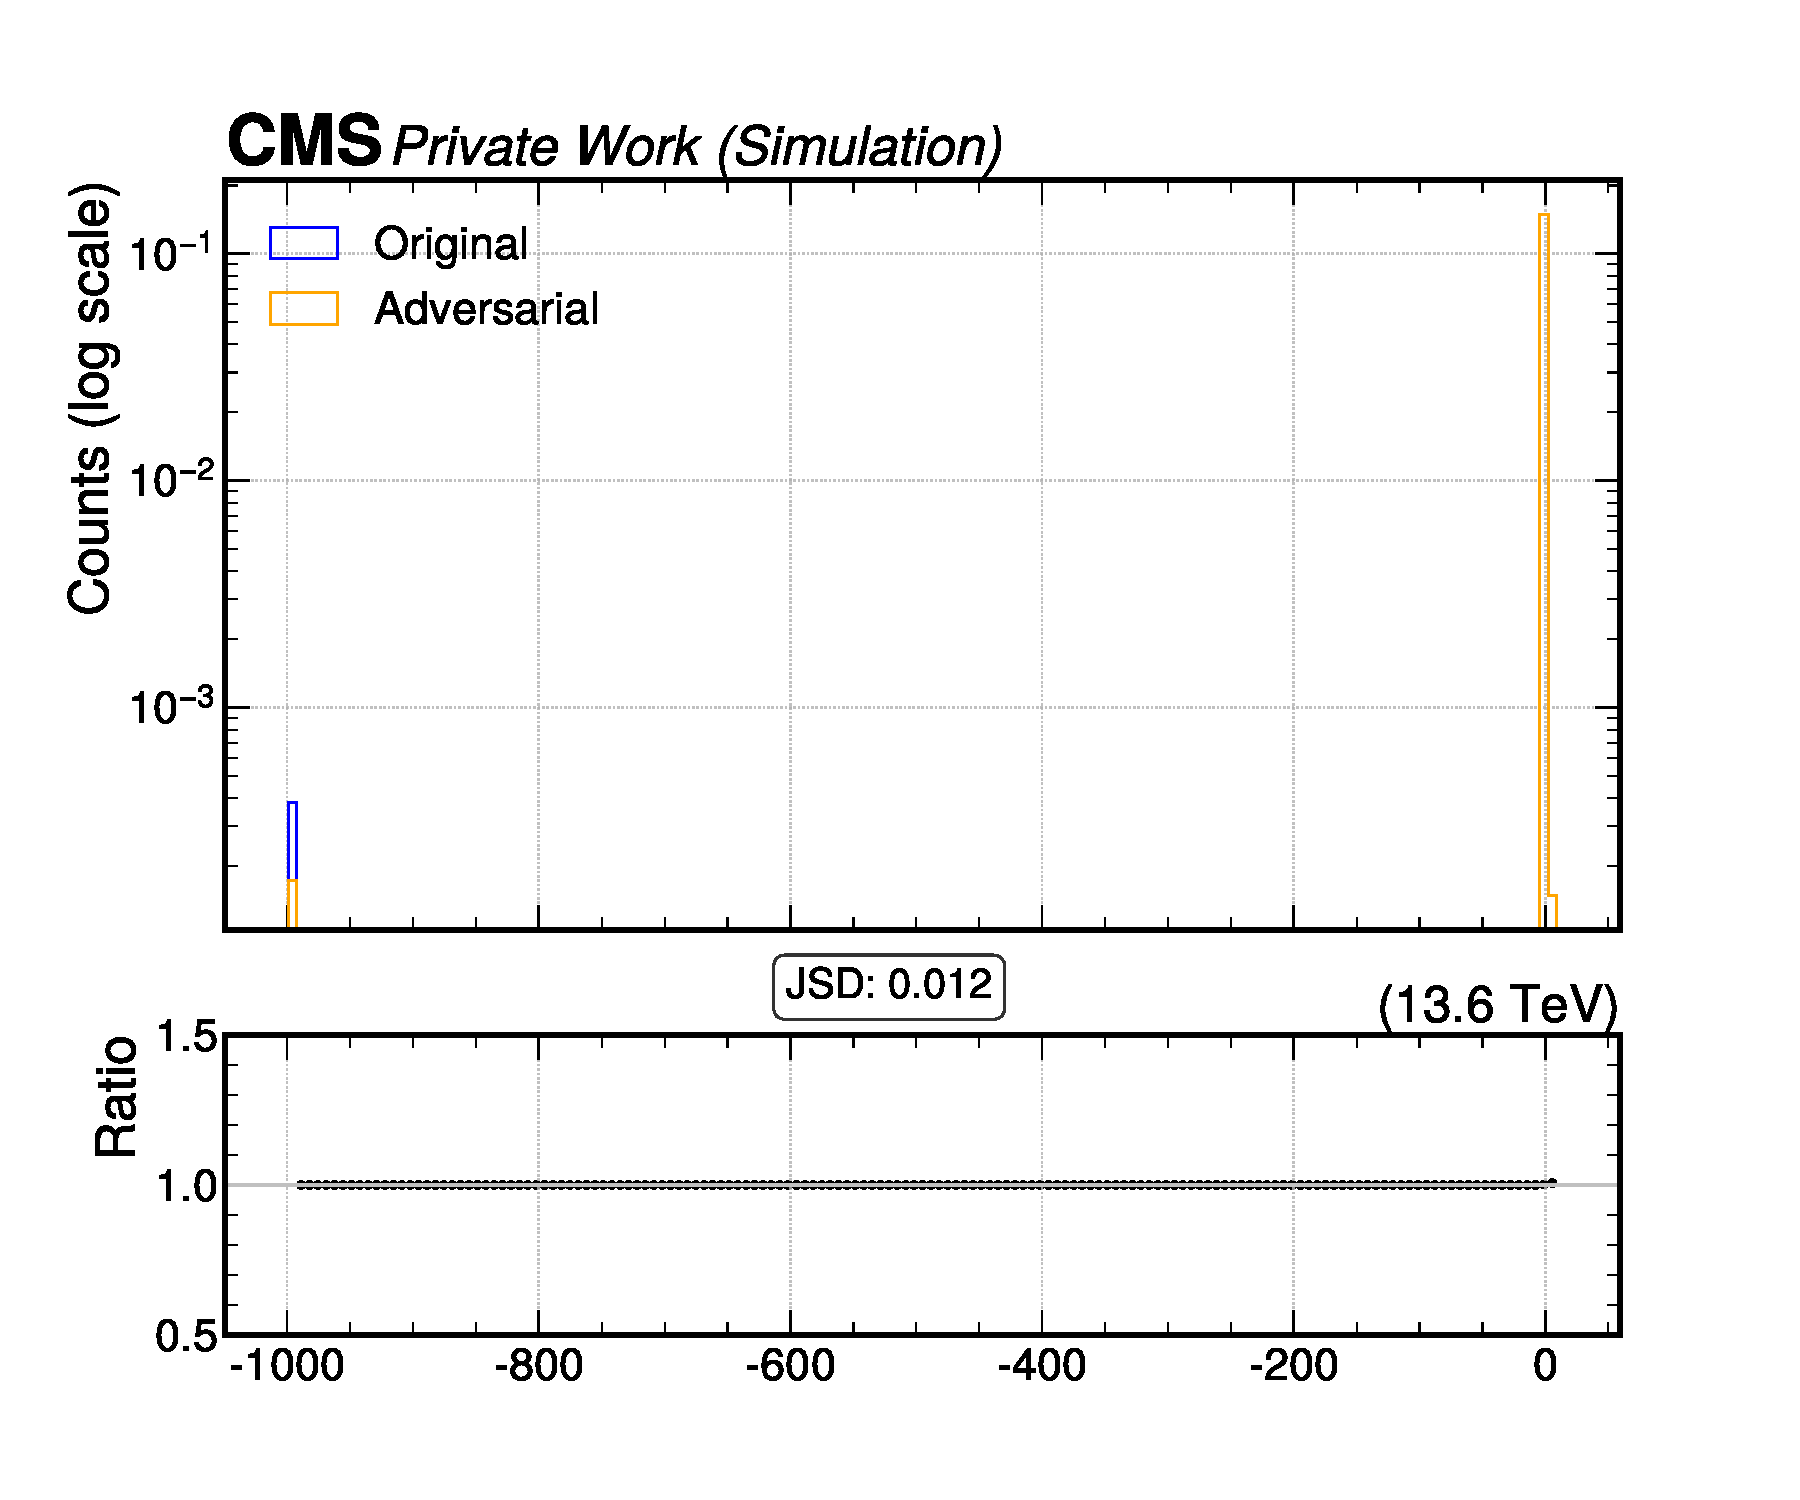
\includegraphics[width=\linewidth]{media/output/features/compare/combined_it_2/cmp_global_features_TagVarCSV_trackSumJetEtRatio.pdf}
    \caption*{Input similarity for PIP-PGD(2).}
  \end{subfigure}\hfill
  \begin{subfigure}[t]{0.32\textwidth}
    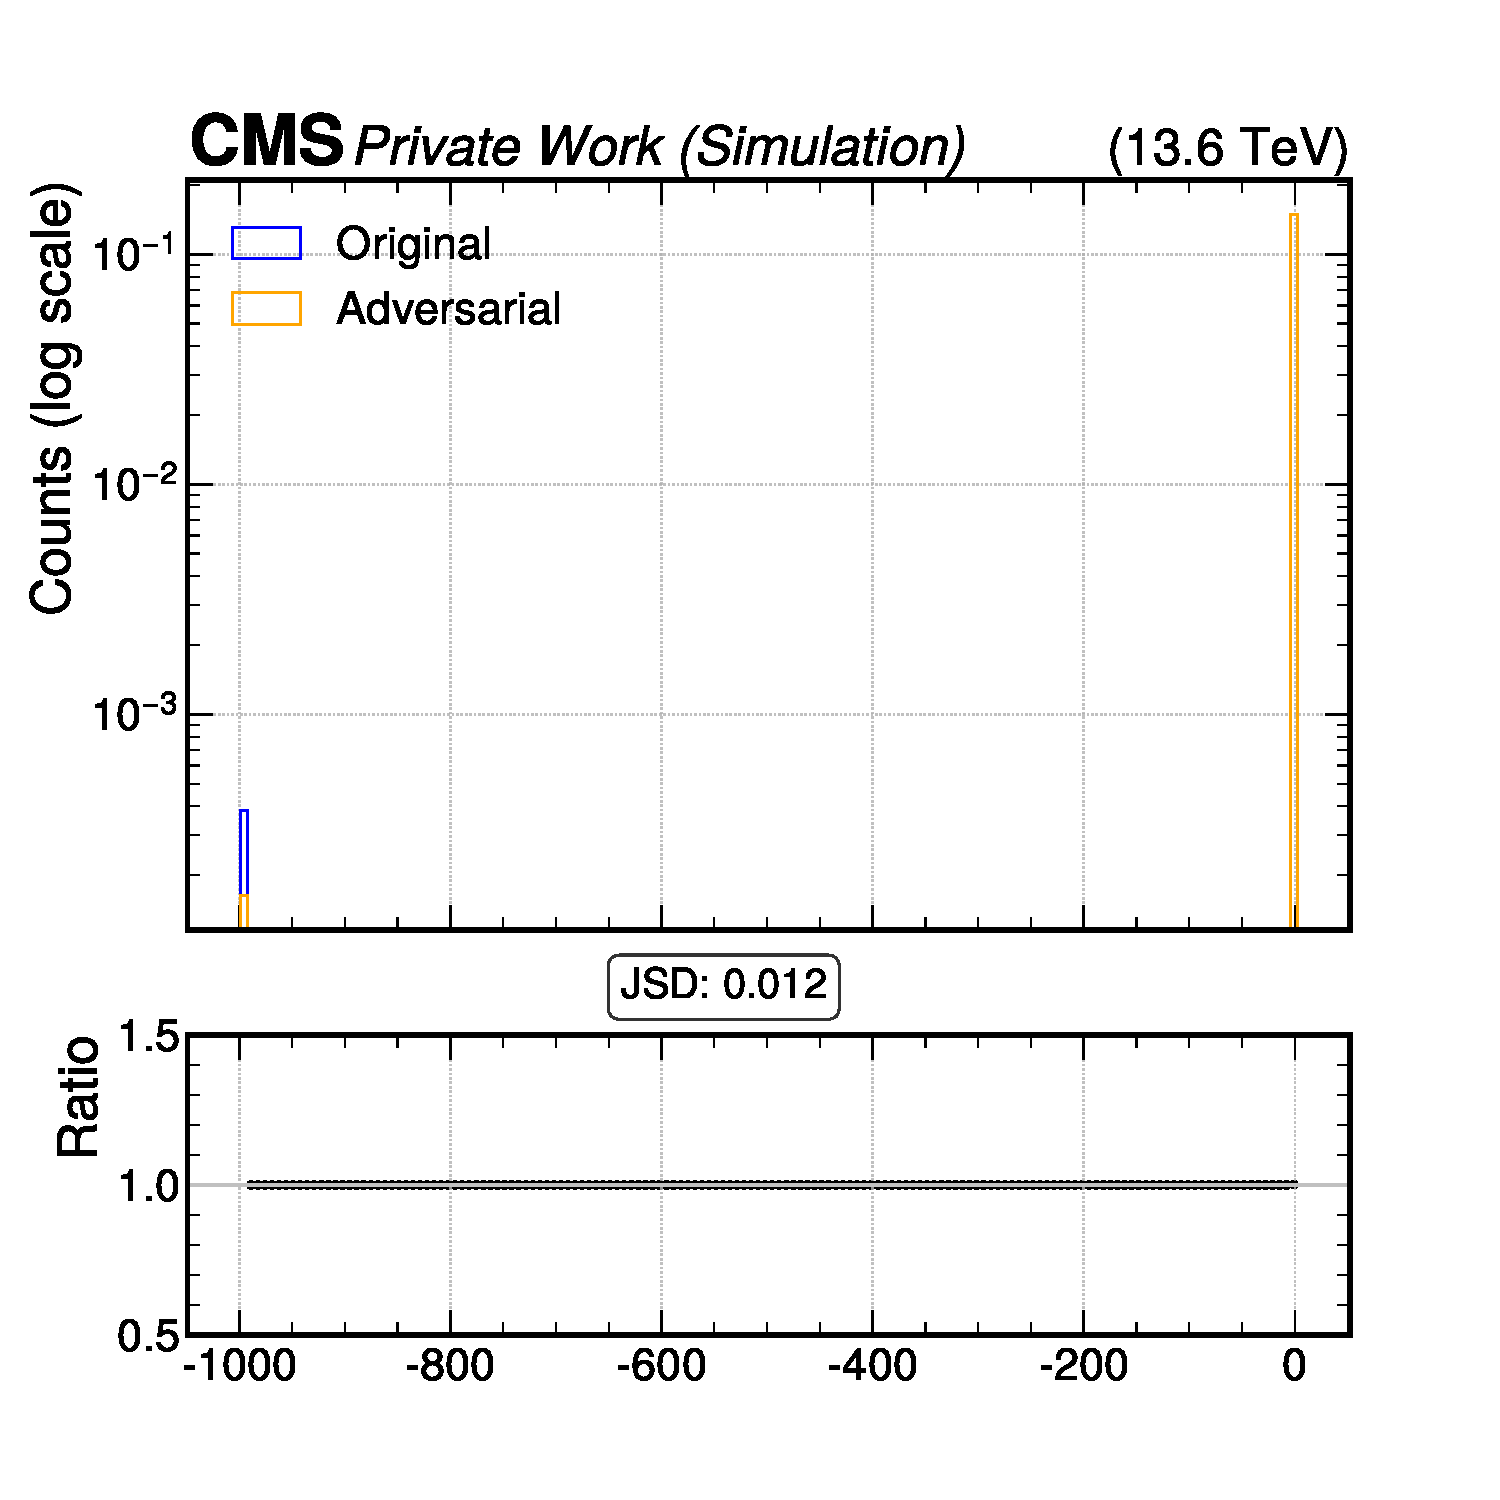
\includegraphics[width=\linewidth]{media/output/features/compare/combined_it_3/cmp_global_features_TagVarCSV_trackSumJetEtRatio.pdf}
    \caption*{Input similarity for PIP-PGD(3).}
  \end{subfigure}

  \caption*{Histogram of \texttt{TagVarCSV\_trackSumJetEtRatio} for multiple iterations of PIP-PGD tested against nominal inputs.}
  \label{fig:combined_input_TagVarCSV_trackSumJetEtRatio}
\end{figure}

\begin{figure}[h]
  \centering
  \begin{subfigure}[t]{0.32\textwidth}
    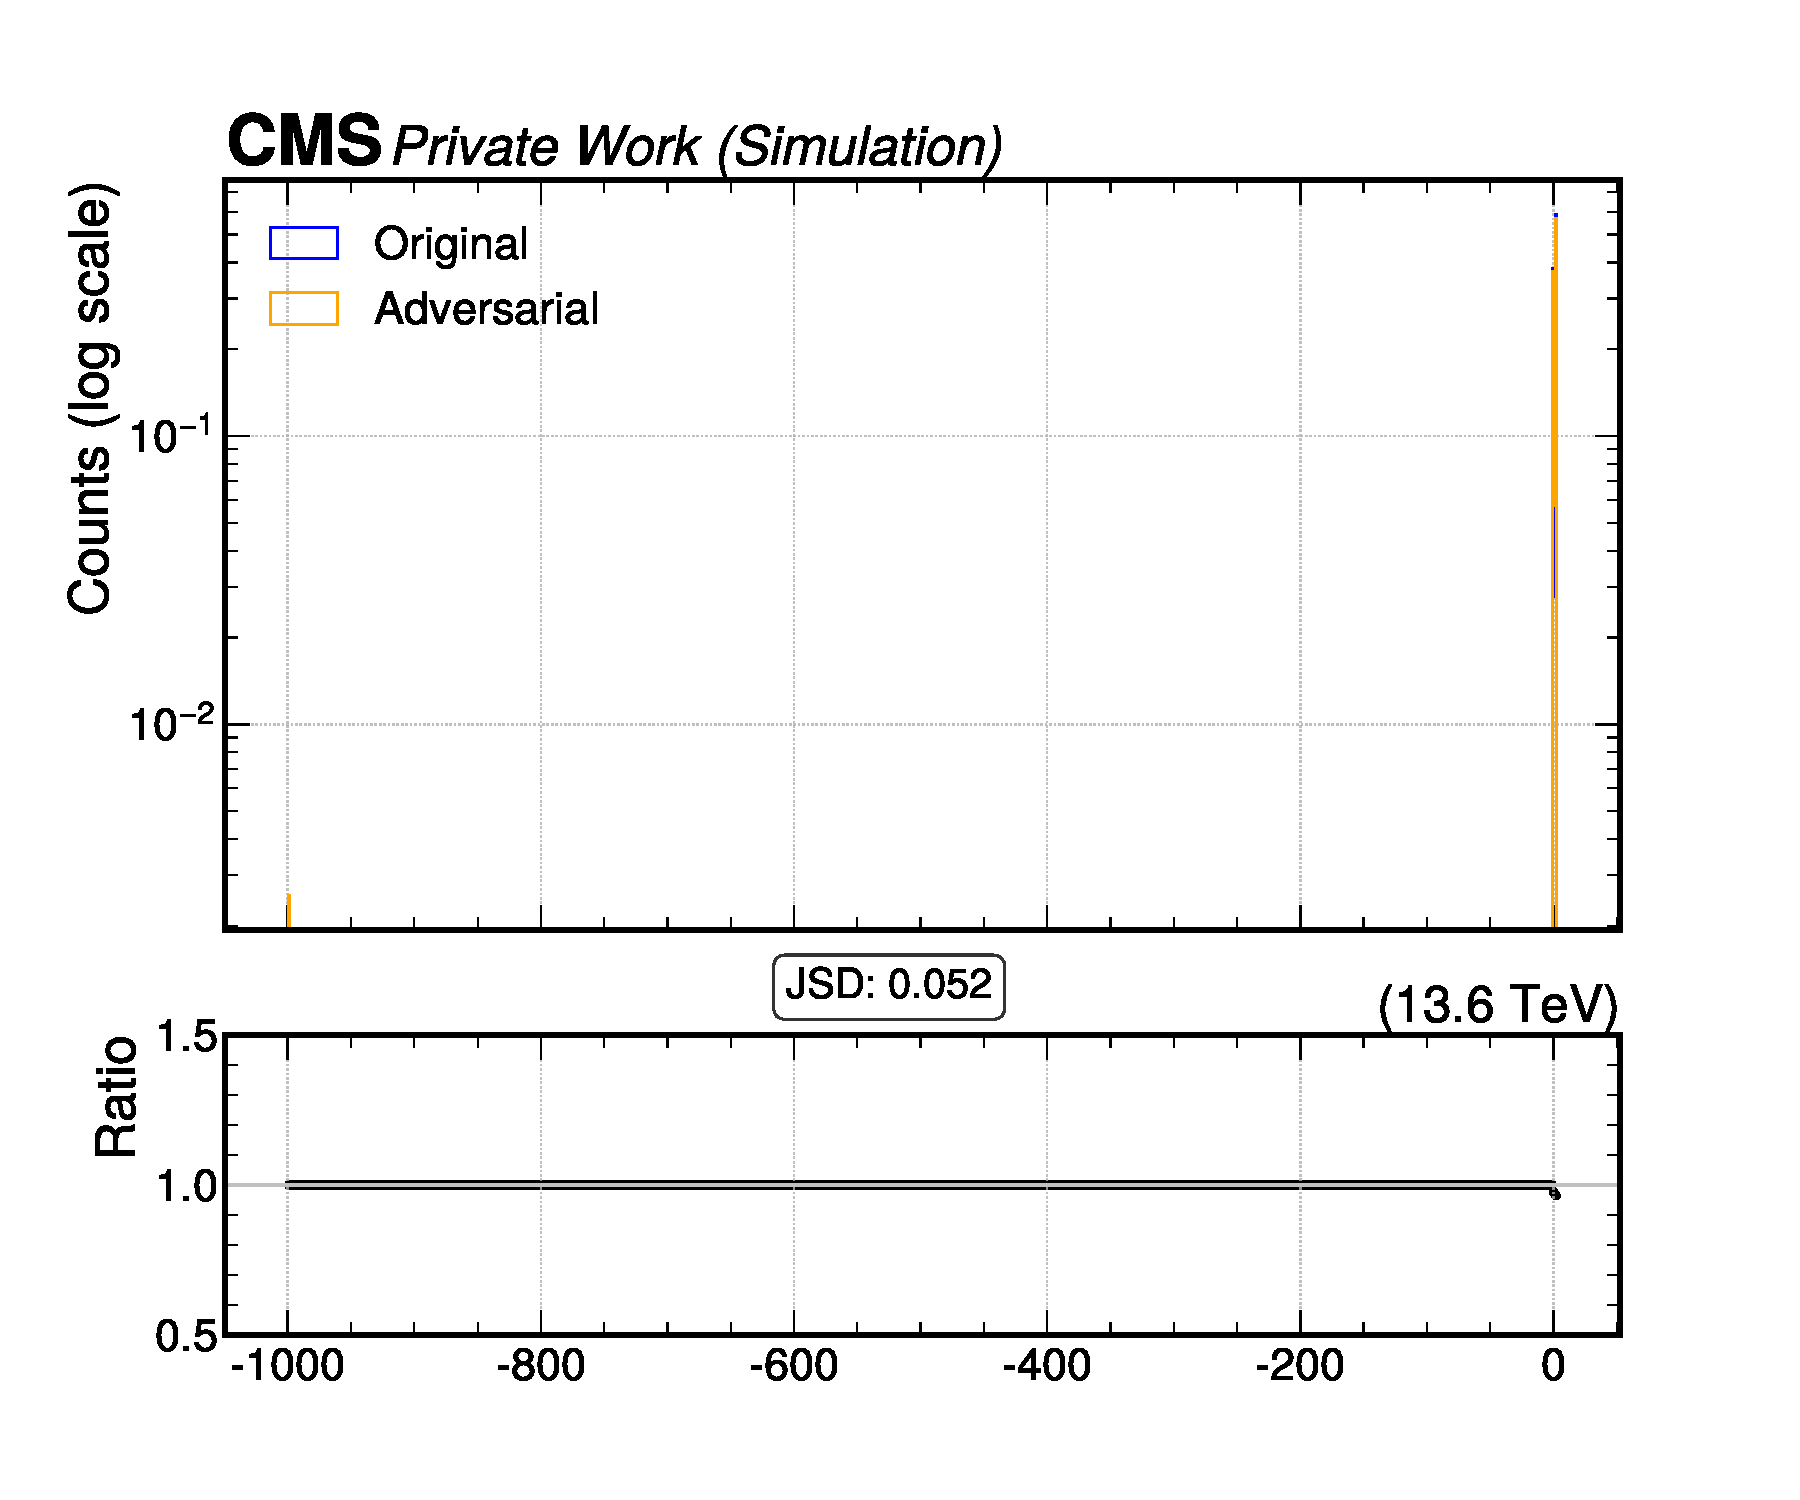
\includegraphics[width=\linewidth]{media/output/features/compare/combined_it_1/cmp_global_features_TagVarCSV_vertexCategory.pdf}
    \caption*{Input similarity for PIP-PGD(1).}
  \end{subfigure}\hfill
  \begin{subfigure}[t]{0.32\textwidth}
    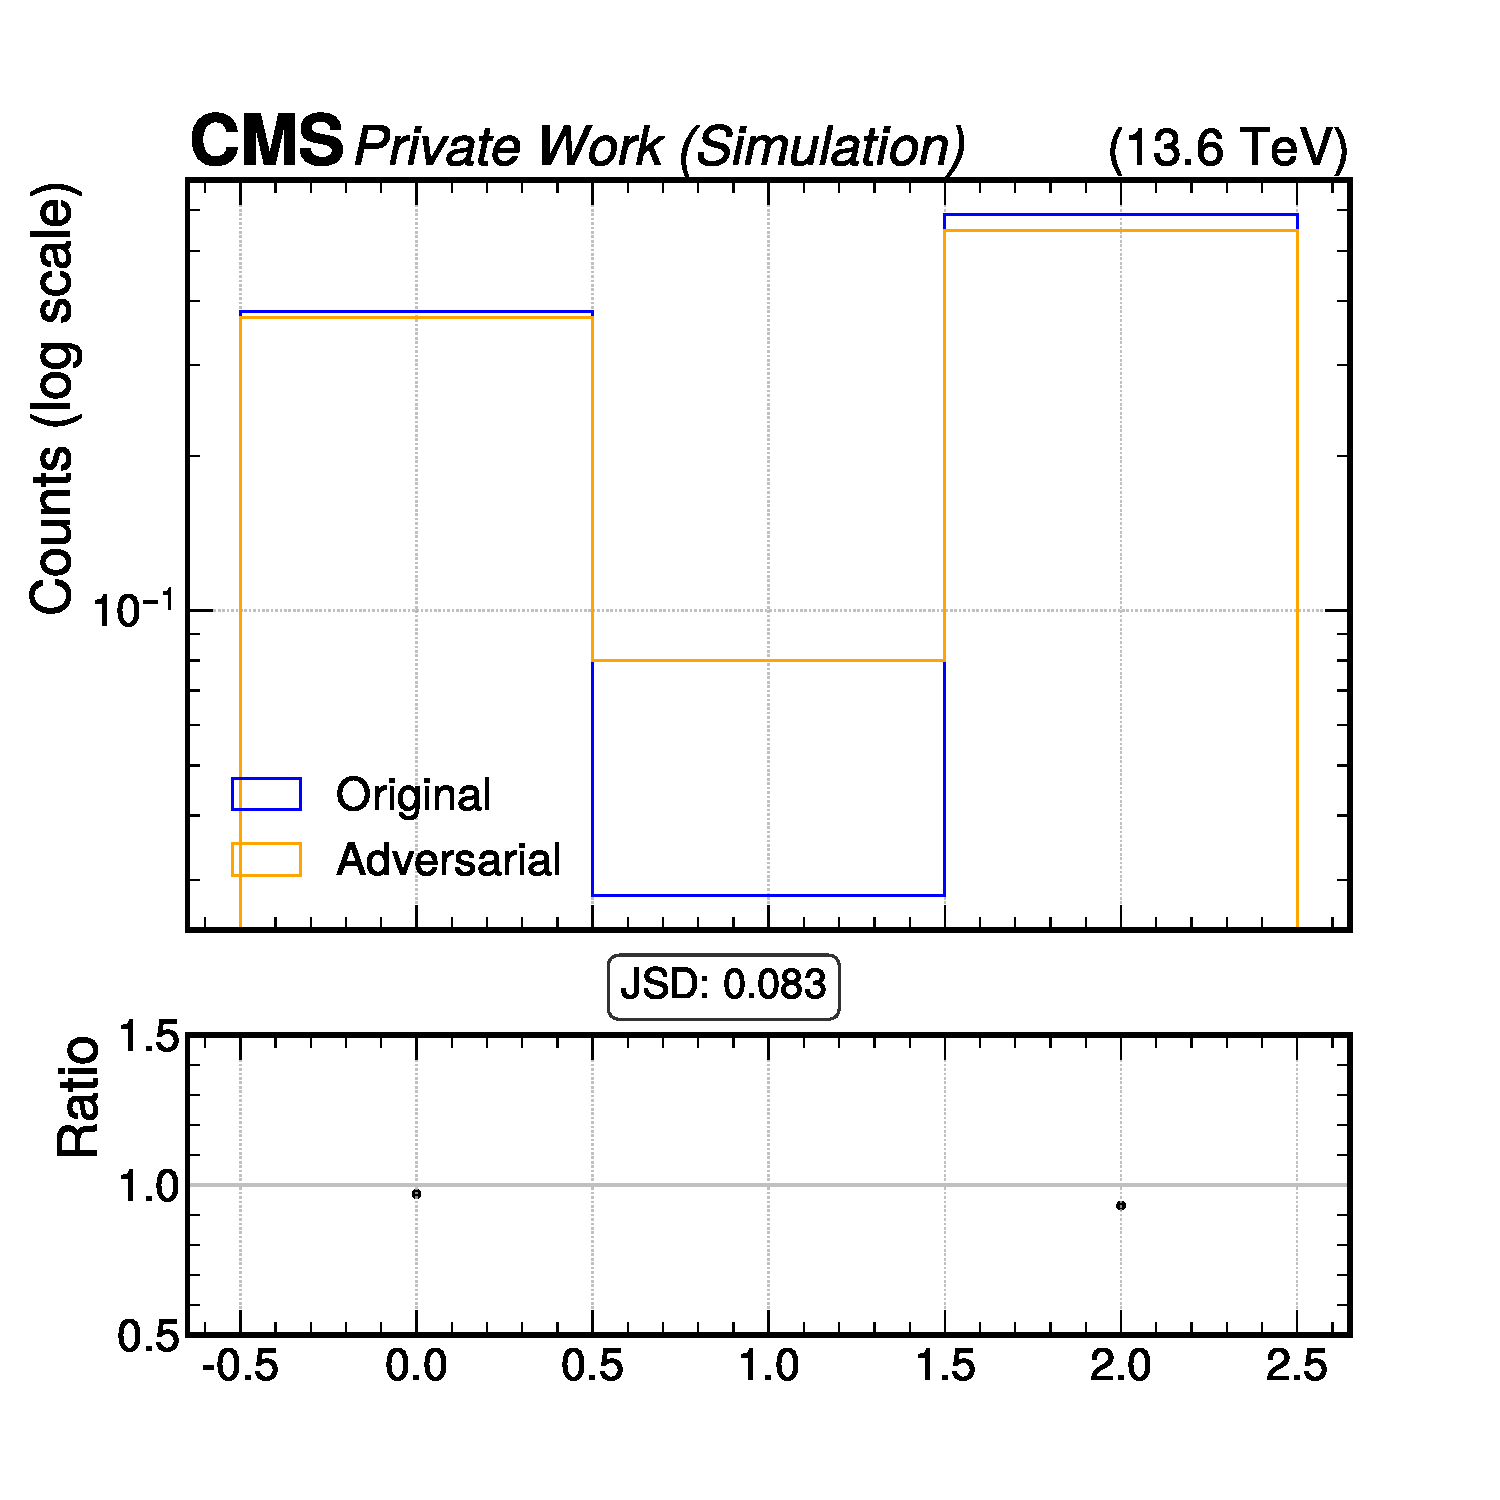
\includegraphics[width=\linewidth]{media/output/features/compare/combined_it_2/cmp_global_features_TagVarCSV_vertexCategory.pdf}
    \caption*{Input similarity for PIP-PGD(2).}
  \end{subfigure}\hfill
  \begin{subfigure}[t]{0.32\textwidth}
    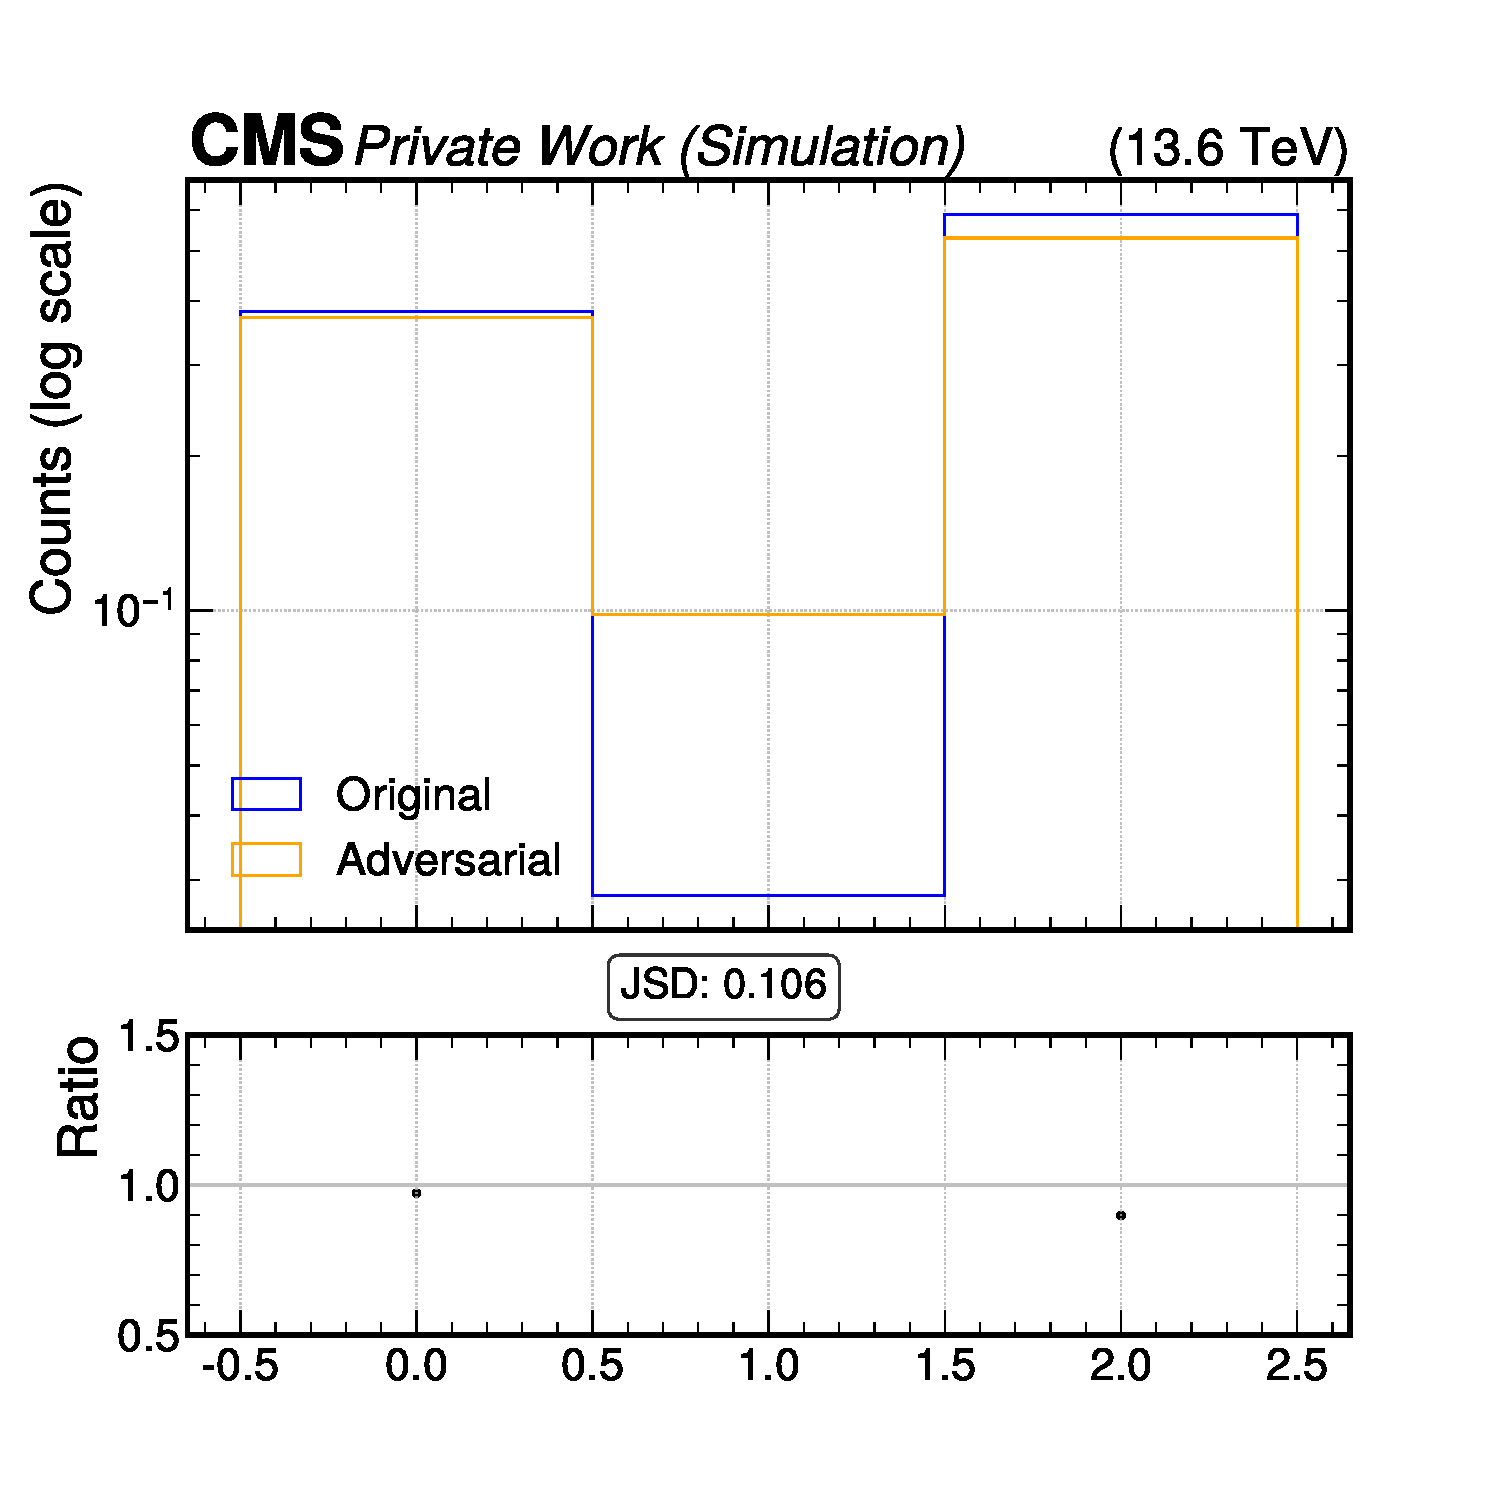
\includegraphics[width=\linewidth]{media/output/features/compare/combined_it_3/cmp_global_features_TagVarCSV_vertexCategory.pdf}
    \caption*{Input similarity for PIP-PGD(3).}
  \end{subfigure}

  \caption*{Histogram of \texttt{TagVarCSV\_vertexCategory} for multiple iterations of PIP-PGD tested against nominal inputs.}
  \label{fig:combined_input_TagVarCSV_vertexCategory}
\end{figure}

\FloatBarrier
\newpage
\subsection*{CPF Features}


\begin{figure}[h]
  \centering
  \begin{subfigure}[t]{0.32\textwidth}
    \includegraphics[width=\linewidth]{media/output/features/compare/combined_it_1/cmp_cpf_arr_Cpfcan_chi2.pdf}
    \caption*{Input similarity for PIP-PGD(1).}
  \end{subfigure}\hfill
  \begin{subfigure}[t]{0.32\textwidth}
    \includegraphics[width=\linewidth]{media/output/features/compare/combined_it_2/cmp_cpf_arr_Cpfcan_chi2.pdf}
    \caption*{Input similarity for PIP-PGD(2).}
  \end{subfigure}\hfill
  \begin{subfigure}[t]{0.32\textwidth}
    \includegraphics[width=\linewidth]{media/output/features/compare/combined_it_3/cmp_cpf_arr_Cpfcan_chi2.pdf}
    \caption*{Input similarity for PIP-PGD(3).}
  \end{subfigure}

  \caption*{Histogram of \texttt{Cpfcan\_chi2} for multiple iterations of PIP-PGD tested against nominal inputs.}
  \label{fig:combined_input_Cpfcan_chi2}
\end{figure}

\begin{figure}[h]
  \centering
  \begin{subfigure}[t]{0.32\textwidth}
    \includegraphics[width=\linewidth]{media/output/features/compare/combined_it_1/cmp_cpf_arr_Cpfcan_chi2.pdf}
    \caption*{Input similarity for PIP-PGD(1).}
  \end{subfigure}\hfill
  \begin{subfigure}[t]{0.32\textwidth}
    \includegraphics[width=\linewidth]{media/output/features/compare/combined_it_2/cmp_cpf_arr_Cpfcan_chi2.pdf}
    \caption*{Input similarity for PIP-PGD(2).}
  \end{subfigure}\hfill
  \begin{subfigure}[t]{0.32\textwidth}
    \includegraphics[width=\linewidth]{media/output/features/compare/combined_it_3/cmp_cpf_arr_Cpfcan_chi2.pdf}
    \caption*{Input similarity for PIP-PGD(3).}
  \end{subfigure}

  \caption*{Histogram of \texttt{Cpfcan\_chi2} for multiple iterations of PIP-PGD tested against nominal inputs.}
  \label{fig:combined_input_Cpfcan_chi2}
\end{figure}

\begin{figure}[h]
  \centering
  \begin{subfigure}[t]{0.32\textwidth}
    \includegraphics[width=\linewidth]{media/output/features/compare/combined_it_1/cmp_cpf_arr_Cpfcan_drminsv.pdf}
    \caption*{Input similarity for PIP-PGD(1).}
  \end{subfigure}\hfill
  \begin{subfigure}[t]{0.32\textwidth}
    \includegraphics[width=\linewidth]{media/output/features/compare/combined_it_2/cmp_cpf_arr_Cpfcan_drminsv.pdf}
    \caption*{Input similarity for PIP-PGD(2).}
  \end{subfigure}\hfill
  \begin{subfigure}[t]{0.32\textwidth}
    \includegraphics[width=\linewidth]{media/output/features/compare/combined_it_3/cmp_cpf_arr_Cpfcan_drminsv.pdf}
    \caption*{Input similarity for PIP-PGD(3).}
  \end{subfigure}

  \caption*{Histogram of \texttt{Cpfcan\_drminsv} for multiple iterations of PIP-PGD tested against nominal inputs.}
  \label{fig:combined_input_Cpfcan_drminsv}
\end{figure}

\begin{figure}[h]
  \centering
  \begin{subfigure}[t]{0.32\textwidth}
    \includegraphics[width=\linewidth]{media/output/features/compare/combined_it_1/cmp_cpf_arr_Cpfcan_ptrel.pdf}
    \caption*{Input similarity for PIP-PGD(1).}
  \end{subfigure}\hfill
  \begin{subfigure}[t]{0.32\textwidth}
    \includegraphics[width=\linewidth]{media/output/features/compare/combined_it_2/cmp_cpf_arr_Cpfcan_ptrel.pdf}
    \caption*{Input similarity for PIP-PGD(2).}
  \end{subfigure}\hfill
  \begin{subfigure}[t]{0.32\textwidth}
    \includegraphics[width=\linewidth]{media/output/features/compare/combined_it_3/cmp_cpf_arr_Cpfcan_ptrel.pdf}
    \caption*{Input similarity for PIP-PGD(3).}
  \end{subfigure}

  \caption*{Histogram of \texttt{Cpfcan\_ptrel} for multiple iterations of PIP-PGD tested against nominal inputs.}
  \label{fig:combined_input_Cpfcan_ptrel}
\end{figure}

\begin{figure}[h]
  \centering
  \begin{subfigure}[t]{0.32\textwidth}
    \includegraphics[width=\linewidth]{media/output/features/compare/combined_it_1/cmp_cpf_arr_Cpfcan_puppiw.pdf}
    \caption*{Input similarity for PIP-PGD(1).}
  \end{subfigure}\hfill
  \begin{subfigure}[t]{0.32\textwidth}
    \includegraphics[width=\linewidth]{media/output/features/compare/combined_it_2/cmp_cpf_arr_Cpfcan_puppiw.pdf}
    \caption*{Input similarity for PIP-PGD(2).}
  \end{subfigure}\hfill
  \begin{subfigure}[t]{0.32\textwidth}
    \includegraphics[width=\linewidth]{media/output/features/compare/combined_it_3/cmp_cpf_arr_Cpfcan_puppiw.pdf}
    \caption*{Input similarity for PIP-PGD(3).}
  \end{subfigure}

  \caption*{Histogram of \texttt{Cpfcan\_puppiw} for multiple iterations of PIP-PGD tested against nominal inputs.}
  \label{fig:combined_input_Cpfcan_puppiw}
\end{figure}

\begin{figure}[h]
  \centering
  \begin{subfigure}[t]{0.32\textwidth}
    \includegraphics[width=\linewidth]{media/output/features/compare/combined_it_1/cmp_cpf_arr_Cpfcan_quality.pdf}
    \caption*{Input similarity for PIP-PGD(1).}
  \end{subfigure}\hfill
  \begin{subfigure}[t]{0.32\textwidth}
    \includegraphics[width=\linewidth]{media/output/features/compare/combined_it_2/cmp_cpf_arr_Cpfcan_quality.pdf}
    \caption*{Input similarity for PIP-PGD(2).}
  \end{subfigure}\hfill
  \begin{subfigure}[t]{0.32\textwidth}
    \includegraphics[width=\linewidth]{media/output/features/compare/combined_it_3/cmp_cpf_arr_Cpfcan_quality.pdf}
    \caption*{Input similarity for PIP-PGD(3).}
  \end{subfigure}

  \caption*{Histogram of \texttt{Cpfcan\_quality} for multiple iterations of PIP-PGD tested against nominal inputs.}
  \label{fig:combined_input_Cpfcan_quality}
\end{figure}

\begin{figure}[h]
  \centering
  \begin{subfigure}[t]{0.32\textwidth}
    \includegraphics[width=\linewidth]{media/output/features/compare/combined_it_1/cmp_cpf_arr_Cpfcan_VTX_ass.pdf}
    \caption*{Input similarity for PIP-PGD(1).}
  \end{subfigure}\hfill
  \begin{subfigure}[t]{0.32\textwidth}
    \includegraphics[width=\linewidth]{media/output/features/compare/combined_it_2/cmp_cpf_arr_Cpfcan_VTX_ass.pdf}
    \caption*{Input similarity for PIP-PGD(2).}
  \end{subfigure}\hfill
  \begin{subfigure}[t]{0.32\textwidth}
    \includegraphics[width=\linewidth]{media/output/features/compare/combined_it_3/cmp_cpf_arr_Cpfcan_VTX_ass.pdf}
    \caption*{Input similarity for PIP-PGD(3).}
  \end{subfigure}

  \caption*{Histogram of \texttt{Cpfcan\_VTX\_ass} for multiple iterations of PIP-PGD tested against nominal inputs.}
  \label{fig:combined_input_Cpfcan_VTX_ass}
\end{figure}

\begin{figure}[h]
  \centering
  \begin{subfigure}[t]{0.32\textwidth}
    \includegraphics[width=\linewidth]{media/output/features/compare/combined_it_1/cmp_cpf_arr_Cpfcan_BtagPf_trackDeltaR.pdf}
    \caption*{Input similarity for PIP-PGD(1).}
  \end{subfigure}\hfill
  \begin{subfigure}[t]{0.32\textwidth}
    \includegraphics[width=\linewidth]{media/output/features/compare/combined_it_2/cmp_cpf_arr_Cpfcan_BtagPf_trackDeltaR.pdf}
    \caption*{Input similarity for PIP-PGD(2).}
  \end{subfigure}\hfill
  \begin{subfigure}[t]{0.32\textwidth}
    \includegraphics[width=\linewidth]{media/output/features/compare/combined_it_3/cmp_cpf_arr_Cpfcan_BtagPf_trackDeltaR.pdf}
    \caption*{Input similarity for PIP-PGD(3).}
  \end{subfigure}

  \caption*{Histogram of \texttt{Cpfcan\_BtagPf\_trackDeltaR} for multiple iterations of PIP-PGD tested against nominal inputs.}
  \label{fig:combined_input_Cpfcan_BtagPf_trackDeltaR}
\end{figure}

\begin{figure}[h]
  \centering
  \begin{subfigure}[t]{0.32\textwidth}
    \includegraphics[width=\linewidth]{media/output/features/compare/combined_it_1/cmp_cpf_arr_Cpfcan_BtagPf_trackEtaRel.pdf}
    \caption*{Input similarity for PIP-PGD(1).}
  \end{subfigure}\hfill
  \begin{subfigure}[t]{0.32\textwidth}
    \includegraphics[width=\linewidth]{media/output/features/compare/combined_it_2/cmp_cpf_arr_Cpfcan_BtagPf_trackEtaRel.pdf}
    \caption*{Input similarity for PIP-PGD(2).}
  \end{subfigure}\hfill
  \begin{subfigure}[t]{0.32\textwidth}
    \includegraphics[width=\linewidth]{media/output/features/compare/combined_it_3/cmp_cpf_arr_Cpfcan_BtagPf_trackEtaRel.pdf}
    \caption*{Input similarity for PIP-PGD(3).}
  \end{subfigure}

  \caption*{Histogram of \texttt{Cpfcan\_BtagPf\_trackEtaRel} for multiple iterations of PIP-PGD tested against nominal inputs.}
  \label{fig:combined_input_Cpfcan_BtagPf_trackEtaRel}
\end{figure}

\begin{figure}[h]
  \centering
  \begin{subfigure}[t]{0.32\textwidth}
    \includegraphics[width=\linewidth]{media/output/features/compare/combined_it_1/cmp_cpf_arr_Cpfcan_BtagPf_trackJetDistVal.pdf}
    \caption*{Input similarity for PIP-PGD(1).}
  \end{subfigure}\hfill
  \begin{subfigure}[t]{0.32\textwidth}
    \includegraphics[width=\linewidth]{media/output/features/compare/combined_it_2/cmp_cpf_arr_Cpfcan_BtagPf_trackJetDistVal.pdf}
    \caption*{Input similarity for PIP-PGD(2).}
  \end{subfigure}\hfill
  \begin{subfigure}[t]{0.32\textwidth}
    \includegraphics[width=\linewidth]{media/output/features/compare/combined_it_3/cmp_cpf_arr_Cpfcan_BtagPf_trackJetDistVal.pdf}
    \caption*{Input similarity for PIP-PGD(3).}
  \end{subfigure}

  \caption*{Histogram of \texttt{Cpfcan\_BtagPf\_trackJetDistVal} for multiple iterations of PIP-PGD tested against nominal inputs.}
  \label{fig:combined_input_Cpfcan_BtagPf_trackJetDistVal}
\end{figure}

\begin{figure}[h]
  \centering
  \begin{subfigure}[t]{0.32\textwidth}
    \includegraphics[width=\linewidth]{media/output/features/compare/combined_it_1/cmp_cpf_arr_Cpfcan_BtagPf_trackPPar.pdf}
    \caption*{Input similarity for PIP-PGD(1).}
  \end{subfigure}\hfill
  \begin{subfigure}[t]{0.32\textwidth}
    \includegraphics[width=\linewidth]{media/output/features/compare/combined_it_2/cmp_cpf_arr_Cpfcan_BtagPf_trackPPar.pdf}
    \caption*{Input similarity for PIP-PGD(2).}
  \end{subfigure}\hfill
  \begin{subfigure}[t]{0.32\textwidth}
    \includegraphics[width=\linewidth]{media/output/features/compare/combined_it_3/cmp_cpf_arr_Cpfcan_BtagPf_trackPPar.pdf}
    \caption*{Input similarity for PIP-PGD(3).}
  \end{subfigure}

  \caption*{Histogram of \texttt{Cpfcan\_BtagPf\_trackPPar} for multiple iterations of PIP-PGD tested against nominal inputs.}
  \label{fig:combined_input_Cpfcan_BtagPf_trackPPar}
\end{figure}

\begin{figure}[h]
  \centering
  \begin{subfigure}[t]{0.32\textwidth}
    \includegraphics[width=\linewidth]{media/output/features/compare/combined_it_1/cmp_cpf_arr_Cpfcan_BtagPf_trackPParRatio.pdf}
    \caption*{Input similarity for PIP-PGD(1).}
  \end{subfigure}\hfill
  \begin{subfigure}[t]{0.32\textwidth}
    \includegraphics[width=\linewidth]{media/output/features/compare/combined_it_2/cmp_cpf_arr_Cpfcan_BtagPf_trackPParRatio.pdf}
    \caption*{Input similarity for PIP-PGD(2).}
  \end{subfigure}\hfill
  \begin{subfigure}[t]{0.32\textwidth}
    \includegraphics[width=\linewidth]{media/output/features/compare/combined_it_3/cmp_cpf_arr_Cpfcan_BtagPf_trackPParRatio.pdf}
    \caption*{Input similarity for PIP-PGD(3).}
  \end{subfigure}

  \caption*{Histogram of \texttt{Cpfcan\_BtagPf\_trackPParRatio} for multiple iterations of PIP-PGD tested against nominal inputs.}
  \label{fig:combined_input_Cpfcan_BtagPf_trackPParRatio}
\end{figure}

\begin{figure}[h]
  \centering
  \begin{subfigure}[t]{0.32\textwidth}
    \includegraphics[width=\linewidth]{media/output/features/compare/combined_it_1/cmp_cpf_arr_Cpfcan_BtagPf_trackPtRel.pdf}
    \caption*{Input similarity for PIP-PGD(1).}
  \end{subfigure}\hfill
  \begin{subfigure}[t]{0.32\textwidth}
    \includegraphics[width=\linewidth]{media/output/features/compare/combined_it_2/cmp_cpf_arr_Cpfcan_BtagPf_trackPtRel.pdf}
    \caption*{Input similarity for PIP-PGD(2).}
  \end{subfigure}\hfill
  \begin{subfigure}[t]{0.32\textwidth}
    \includegraphics[width=\linewidth]{media/output/features/compare/combined_it_3/cmp_cpf_arr_Cpfcan_BtagPf_trackPtRel.pdf}
    \caption*{Input similarity for PIP-PGD(3).}
  \end{subfigure}

  \caption*{Histogram of \texttt{Cpfcan\_BtagPf\_trackPtRel} for multiple iterations of PIP-PGD tested against nominal inputs.}
  \label{fig:combined_input_Cpfcan_BtagPf_trackPtRel}
\end{figure}

\begin{figure}[h]
  \centering
  \begin{subfigure}[t]{0.32\textwidth}
    \includegraphics[width=\linewidth]{media/output/features/compare/combined_it_1/cmp_cpf_arr_Cpfcan_BtagPf_trackSip2dSig.pdf}
    \caption*{Input similarity for PIP-PGD(1).}
  \end{subfigure}\hfill
  \begin{subfigure}[t]{0.32\textwidth}
    \includegraphics[width=\linewidth]{media/output/features/compare/combined_it_2/cmp_cpf_arr_Cpfcan_BtagPf_trackSip2dSig.pdf}
    \caption*{Input similarity for PIP-PGD(2).}
  \end{subfigure}\hfill
  \begin{subfigure}[t]{0.32\textwidth}
    \includegraphics[width=\linewidth]{media/output/features/compare/combined_it_3/cmp_cpf_arr_Cpfcan_BtagPf_trackSip2dSig.pdf}
    \caption*{Input similarity for PIP-PGD(3).}
  \end{subfigure}

  \caption*{Histogram of \texttt{Cpfcan\_BtagPf\_trackSip2dSig} for multiple iterations of PIP-PGD tested against nominal inputs.}
  \label{fig:combined_input_Cpfcan_BtagPf_trackSip2dSig}
\end{figure}

\begin{figure}[h]
  \centering
  \begin{subfigure}[t]{0.32\textwidth}
    \includegraphics[width=\linewidth]{media/output/features/compare/combined_it_1/cmp_cpf_arr_Cpfcan_BtagPf_trackSip2dVal.pdf}
    \caption*{Input similarity for PIP-PGD(1).}
  \end{subfigure}\hfill
  \begin{subfigure}[t]{0.32\textwidth}
    \includegraphics[width=\linewidth]{media/output/features/compare/combined_it_2/cmp_cpf_arr_Cpfcan_BtagPf_trackSip2dVal.pdf}
    \caption*{Input similarity for PIP-PGD(2).}
  \end{subfigure}\hfill
  \begin{subfigure}[t]{0.32\textwidth}
    \includegraphics[width=\linewidth]{media/output/features/compare/combined_it_3/cmp_cpf_arr_Cpfcan_BtagPf_trackSip2dVal.pdf}
    \caption*{Input similarity for PIP-PGD(3).}
  \end{subfigure}

  \caption*{Histogram of \texttt{Cpfcan\_BtagPf\_trackSip2dVal} for multiple iterations of PIP-PGD tested against nominal inputs.}
  \label{fig:combined_input_Cpfcan_BtagPf_trackSip2dVal}
\end{figure}

\begin{figure}[h]
  \centering
  \begin{subfigure}[t]{0.32\textwidth}
    \includegraphics[width=\linewidth]{media/output/features/compare/combined_it_1/cmp_cpf_arr_Cpfcan_BtagPf_trackSip3dSig.pdf}
    \caption*{Input similarity for PIP-PGD(1).}
  \end{subfigure}\hfill
  \begin{subfigure}[t]{0.32\textwidth}
    \includegraphics[width=\linewidth]{media/output/features/compare/combined_it_2/cmp_cpf_arr_Cpfcan_BtagPf_trackSip3dSig.pdf}
    \caption*{Input similarity for PIP-PGD(2).}
  \end{subfigure}\hfill
  \begin{subfigure}[t]{0.32\textwidth}
    \includegraphics[width=\linewidth]{media/output/features/compare/combined_it_3/cmp_cpf_arr_Cpfcan_BtagPf_trackSip3dSig.pdf}
    \caption*{Input similarity for PIP-PGD(3).}
  \end{subfigure}

  \caption*{Histogram of \texttt{Cpfcan\_BtagPf\_trackSip3dSig} for multiple iterations of PIP-PGD tested against nominal inputs.}
  \label{fig:combined_input_Cpfcan_BtagPf_trackSip3dSig}
\end{figure}

\begin{figure}[h]
  \centering
  \begin{subfigure}[t]{0.32\textwidth}
    \includegraphics[width=\linewidth]{media/output/features/compare/combined_it_1/cmp_cpf_arr_Cpfcan_BtagPf_trackSip3dVal.pdf}
    \caption*{Input similarity for PIP-PGD(1).}
  \end{subfigure}\hfill
  \begin{subfigure}[t]{0.32\textwidth}
    \includegraphics[width=\linewidth]{media/output/features/compare/combined_it_2/cmp_cpf_arr_Cpfcan_BtagPf_trackSip3dVal.pdf}
    \caption*{Input similarity for PIP-PGD(2).}
  \end{subfigure}\hfill
  \begin{subfigure}[t]{0.32\textwidth}
    \includegraphics[width=\linewidth]{media/output/features/compare/combined_it_3/cmp_cpf_arr_Cpfcan_BtagPf_trackSip3dVal.pdf}
    \caption*{Input similarity for PIP-PGD(3).}
  \end{subfigure}

  \caption*{Histogram of \texttt{Cpfcan\_BtagPf\_trackSip3dVal} for multiple iterations of PIP-PGD tested against nominal inputs.}
  \label{fig:combined_input_Cpfcan_BtagPf_trackSip3dVal}
\end{figure}

\FloatBarrier
\newpage
\subsection*{NPF Features}


\begin{figure}[h]
  \centering
  \begin{subfigure}[t]{0.32\textwidth}
    \includegraphics[width=\linewidth]{media/output/features/compare/combined_it_1/cmp_npf_arr_Npfcan_deltaR.pdf}
    \caption*{Input similarity for PIP-PGD(1).}
  \end{subfigure}\hfill
  \begin{subfigure}[t]{0.32\textwidth}
    \includegraphics[width=\linewidth]{media/output/features/compare/combined_it_2/cmp_npf_arr_Npfcan_deltaR.pdf}
    \caption*{Input similarity for PIP-PGD(2).}
  \end{subfigure}\hfill
  \begin{subfigure}[t]{0.32\textwidth}
    \includegraphics[width=\linewidth]{media/output/features/compare/combined_it_3/cmp_npf_arr_Npfcan_deltaR.pdf}
    \caption*{Input similarity for PIP-PGD(3).}
  \end{subfigure}

  \caption*{Histogram of \texttt{Npfcan\_deltaR} for multiple iterations of PIP-PGD tested against nominal inputs.}
  \label{fig:combined_input_Npfcan_deltaR}
\end{figure}

\begin{figure}[h]
  \centering
  \begin{subfigure}[t]{0.32\textwidth}
    \includegraphics[width=\linewidth]{media/output/features/compare/combined_it_1/cmp_npf_arr_Npfcan_drminsv.pdf}
    \caption*{Input similarity for PIP-PGD(1).}
  \end{subfigure}\hfill
  \begin{subfigure}[t]{0.32\textwidth}
    \includegraphics[width=\linewidth]{media/output/features/compare/combined_it_2/cmp_npf_arr_Npfcan_drminsv.pdf}
    \caption*{Input similarity for PIP-PGD(2).}
  \end{subfigure}\hfill
  \begin{subfigure}[t]{0.32\textwidth}
    \includegraphics[width=\linewidth]{media/output/features/compare/combined_it_3/cmp_npf_arr_Npfcan_drminsv.pdf}
    \caption*{Input similarity for PIP-PGD(3).}
  \end{subfigure}

  \caption*{Histogram of \texttt{Npfcan\_drminsv} for multiple iterations of PIP-PGD tested against nominal inputs.}
  \label{fig:combined_input_Npfcan_drminsv}
\end{figure}

\begin{figure}[h]
  \centering
  \begin{subfigure}[t]{0.32\textwidth}
    \includegraphics[width=\linewidth]{media/output/features/compare/combined_it_1/cmp_npf_arr_Npfcan_HadFrac.pdf}
    \caption*{Input similarity for PIP-PGD(1).}
  \end{subfigure}\hfill
  \begin{subfigure}[t]{0.32\textwidth}
    \includegraphics[width=\linewidth]{media/output/features/compare/combined_it_2/cmp_npf_arr_Npfcan_HadFrac.pdf}
    \caption*{Input similarity for PIP-PGD(2).}
  \end{subfigure}\hfill
  \begin{subfigure}[t]{0.32\textwidth}
    \includegraphics[width=\linewidth]{media/output/features/compare/combined_it_3/cmp_npf_arr_Npfcan_HadFrac.pdf}
    \caption*{Input similarity for PIP-PGD(3).}
  \end{subfigure}

  \caption*{Histogram of \texttt{Npfcan\_HadFrac} for multiple iterations of PIP-PGD tested against nominal inputs.}
  \label{fig:combined_input_Npfcan_HadFrac}
\end{figure}

\begin{figure}[h]
  \centering
  \begin{subfigure}[t]{0.32\textwidth}
    \includegraphics[width=\linewidth]{media/output/features/compare/combined_it_1/cmp_npf_arr_Npfcan_isGamma.pdf}
    \caption*{Input similarity for PIP-PGD(1).}
  \end{subfigure}\hfill
  \begin{subfigure}[t]{0.32\textwidth}
    \includegraphics[width=\linewidth]{media/output/features/compare/combined_it_2/cmp_npf_arr_Npfcan_isGamma.pdf}
    \caption*{Input similarity for PIP-PGD(2).}
  \end{subfigure}\hfill
  \begin{subfigure}[t]{0.32\textwidth}
    \includegraphics[width=\linewidth]{media/output/features/compare/combined_it_3/cmp_npf_arr_Npfcan_isGamma.pdf}
    \caption*{Input similarity for PIP-PGD(3).}
  \end{subfigure}

  \caption*{Histogram of \texttt{Npfcan\_isGamma} for multiple iterations of PIP-PGD tested against nominal inputs.}
  \label{fig:combined_input_Npfcan_isGamma}
\end{figure}

\begin{figure}[h]
  \centering
  \begin{subfigure}[t]{0.32\textwidth}
    \includegraphics[width=\linewidth]{media/output/features/compare/combined_it_1/cmp_npf_arr_Npfcan_ptrel.pdf}
    \caption*{Input similarity for PIP-PGD(1).}
  \end{subfigure}\hfill
  \begin{subfigure}[t]{0.32\textwidth}
    \includegraphics[width=\linewidth]{media/output/features/compare/combined_it_2/cmp_npf_arr_Npfcan_ptrel.pdf}
    \caption*{Input similarity for PIP-PGD(2).}
  \end{subfigure}\hfill
  \begin{subfigure}[t]{0.32\textwidth}
    \includegraphics[width=\linewidth]{media/output/features/compare/combined_it_3/cmp_npf_arr_Npfcan_ptrel.pdf}
    \caption*{Input similarity for PIP-PGD(3).}
  \end{subfigure}

  \caption*{Histogram of \texttt{Npfcan\_ptrel} for multiple iterations of PIP-PGD tested against nominal inputs.}
  \label{fig:combined_input_Npfcan_ptrel}
\end{figure}

\begin{figure}[h]
  \centering
  \begin{subfigure}[t]{0.32\textwidth}
    \includegraphics[width=\linewidth]{media/output/features/compare/combined_it_1/cmp_npf_arr_Npfcan_puppiw.pdf}
    \caption*{Input similarity for PIP-PGD(1).}
  \end{subfigure}\hfill
  \begin{subfigure}[t]{0.32\textwidth}
    \includegraphics[width=\linewidth]{media/output/features/compare/combined_it_2/cmp_npf_arr_Npfcan_puppiw.pdf}
    \caption*{Input similarity for PIP-PGD(2).}
  \end{subfigure}\hfill
  \begin{subfigure}[t]{0.32\textwidth}
    \includegraphics[width=\linewidth]{media/output/features/compare/combined_it_3/cmp_npf_arr_Npfcan_puppiw.pdf}
    \caption*{Input similarity for PIP-PGD(3).}
  \end{subfigure}

  \caption*{Histogram of \texttt{Npfcan\_puppiw} for multiple iterations of PIP-PGD tested against nominal inputs.}
  \label{fig:combined_input_Npfcan_puppiw}
\end{figure}

\FloatBarrier
\newpage
\subsection*{SV Features}

\begin{figure}[h]
  \centering
  \begin{subfigure}[t]{0.32\textwidth}
    \includegraphics[width=\linewidth]{media/output/features/compare/combined_it_1/cmp_vtx_arr_sv_chi2.pdf}
    \caption*{Input similarity for PIP-PGD(1).}
  \end{subfigure}\hfill
  \begin{subfigure}[t]{0.32\textwidth}
    \includegraphics[width=\linewidth]{media/output/features/compare/combined_it_2/cmp_vtx_arr_sv_chi2.pdf}
    \caption*{Input similarity for PIP-PGD(2).}
  \end{subfigure}\hfill
  \begin{subfigure}[t]{0.32\textwidth}
    \includegraphics[width=\linewidth]{media/output/features/compare/combined_it_3/cmp_vtx_arr_sv_chi2.pdf}
    \caption*{Input similarity for PIP-PGD(3).}
  \end{subfigure}

  \caption*{Histogram of \texttt{sv\_chi2} for multiple iterations of PIP-PGD tested against nominal inputs.}
  \label{fig:combined_input_sv_chi2}
\end{figure}

\begin{figure}[h]
  \centering
  \begin{subfigure}[t]{0.32\textwidth}
    \includegraphics[width=\linewidth]{media/output/features/compare/combined_it_1/cmp_vtx_arr_sv_costhetasvpv.pdf}
    \caption*{Input similarity for PIP-PGD(1).}
  \end{subfigure}\hfill
  \begin{subfigure}[t]{0.32\textwidth}
    \includegraphics[width=\linewidth]{media/output/features/compare/combined_it_2/cmp_vtx_arr_sv_costhetasvpv.pdf}
    \caption*{Input similarity for PIP-PGD(2).}
  \end{subfigure}\hfill
  \begin{subfigure}[t]{0.32\textwidth}
    \includegraphics[width=\linewidth]{media/output/features/compare/combined_it_3/cmp_vtx_arr_sv_costhetasvpv.pdf}
    \caption*{Input similarity for PIP-PGD(3).}
  \end{subfigure}

  \caption*{Histogram of \texttt{sv\_costhetasvpv} for multiple iterations of PIP-PGD tested against nominal inputs.}
  \label{fig:combined_input_sv_costhetasvpv}
\end{figure}

\begin{figure}[h]
  \centering
  \begin{subfigure}[t]{0.32\textwidth}
    \includegraphics[width=\linewidth]{media/output/features/compare/combined_it_1/cmp_vtx_arr_sv_d3d.pdf}
    \caption*{Input similarity for PIP-PGD(1).}
  \end{subfigure}\hfill
  \begin{subfigure}[t]{0.32\textwidth}
    \includegraphics[width=\linewidth]{media/output/features/compare/combined_it_2/cmp_vtx_arr_sv_d3d.pdf}
    \caption*{Input similarity for PIP-PGD(2).}
  \end{subfigure}\hfill
  \begin{subfigure}[t]{0.32\textwidth}
    \includegraphics[width=\linewidth]{media/output/features/compare/combined_it_3/cmp_vtx_arr_sv_d3d.pdf}
    \caption*{Input similarity for PIP-PGD(3).}
  \end{subfigure}

  \caption*{Histogram of \texttt{sv\_d3d} for multiple iterations of PIP-PGD tested against nominal inputs.}
  \label{fig:combined_input_sv_d3d}
\end{figure}

\begin{figure}[h]
  \centering
  \begin{subfigure}[t]{0.32\textwidth}
    \includegraphics[width=\linewidth]{media/output/features/compare/combined_it_1/cmp_vtx_arr_sv_d3dsig.pdf}
    \caption*{Input similarity for PIP-PGD(1).}
  \end{subfigure}\hfill
  \begin{subfigure}[t]{0.32\textwidth}
    \includegraphics[width=\linewidth]{media/output/features/compare/combined_it_2/cmp_vtx_arr_sv_d3dsig.pdf}
    \caption*{Input similarity for PIP-PGD(2).}
  \end{subfigure}\hfill
  \begin{subfigure}[t]{0.32\textwidth}
    \includegraphics[width=\linewidth]{media/output/features/compare/combined_it_3/cmp_vtx_arr_sv_d3dsig.pdf}
    \caption*{Input similarity for PIP-PGD(3).}
  \end{subfigure}

  \caption*{Histogram of \texttt{sv\_d3dsig} for multiple iterations of PIP-PGD tested against nominal inputs.}
  \label{fig:combined_input_sv_d3dsig}
\end{figure}

\begin{figure}[h]
  \centering
  \begin{subfigure}[t]{0.32\textwidth}
    \includegraphics[width=\linewidth]{media/output/features/compare/combined_it_1/cmp_vtx_arr_sv_deltaR.pdf}
    \caption*{Input similarity for PIP-PGD(1).}
  \end{subfigure}\hfill
  \begin{subfigure}[t]{0.32\textwidth}
    \includegraphics[width=\linewidth]{media/output/features/compare/combined_it_2/cmp_vtx_arr_sv_deltaR.pdf}
    \caption*{Input similarity for PIP-PGD(2).}
  \end{subfigure}\hfill
  \begin{subfigure}[t]{0.32\textwidth}
    \includegraphics[width=\linewidth]{media/output/features/compare/combined_it_3/cmp_vtx_arr_sv_deltaR.pdf}
    \caption*{Input similarity for PIP-PGD(3).}
  \end{subfigure}

  \caption*{Histogram of \texttt{sv\_deltaR} for multiple iterations of PIP-PGD tested against nominal inputs.}
  \label{fig:combined_input_sv_deltaR}
\end{figure}

\begin{figure}[h]
  \centering
  \begin{subfigure}[t]{0.32\textwidth}
    \includegraphics[width=\linewidth]{media/output/features/compare/combined_it_1/cmp_vtx_arr_sv_dxy.pdf}
    \caption*{Input similarity for PIP-PGD(1).}
  \end{subfigure}\hfill
  \begin{subfigure}[t]{0.32\textwidth}
    \includegraphics[width=\linewidth]{media/output/features/compare/combined_it_2/cmp_vtx_arr_sv_dxy.pdf}
    \caption*{Input similarity for PIP-PGD(2).}
  \end{subfigure}\hfill
  \begin{subfigure}[t]{0.32\textwidth}
    \includegraphics[width=\linewidth]{media/output/features/compare/combined_it_3/cmp_vtx_arr_sv_dxy.pdf}
    \caption*{Input similarity for PIP-PGD(3).}
  \end{subfigure}

  \caption*{Histogram of \texttt{sv\_dxy} for multiple iterations of PIP-PGD tested against nominal inputs.}
  \label{fig:combined_input_sv_dxy}
\end{figure}

\begin{figure}[h]
  \centering
  \begin{subfigure}[t]{0.32\textwidth}
    \includegraphics[width=\linewidth]{media/output/features/compare/combined_it_1/cmp_vtx_arr_sv_dxysig.pdf}
    \caption*{Input similarity for PIP-PGD(1).}
  \end{subfigure}\hfill
  \begin{subfigure}[t]{0.32\textwidth}
    \includegraphics[width=\linewidth]{media/output/features/compare/combined_it_2/cmp_vtx_arr_sv_dxysig.pdf}
    \caption*{Input similarity for PIP-PGD(2).}
  \end{subfigure}\hfill
  \begin{subfigure}[t]{0.32\textwidth}
    \includegraphics[width=\linewidth]{media/output/features/compare/combined_it_3/cmp_vtx_arr_sv_dxysig.pdf}
    \caption*{Input similarity for PIP-PGD(3).}
  \end{subfigure}

  \caption*{Histogram of \texttt{sv\_dxysig} for multiple iterations of PIP-PGD tested against nominal inputs.}
  \label{fig:combined_input_sv_dxysig}
\end{figure}

\begin{figure}[h]
  \centering
  \begin{subfigure}[t]{0.32\textwidth}
    \includegraphics[width=\linewidth]{media/output/features/compare/combined_it_1/cmp_vtx_arr_sv_enratio.pdf}
    \caption*{Input similarity for PIP-PGD(1).}
  \end{subfigure}\hfill
  \begin{subfigure}[t]{0.32\textwidth}
    \includegraphics[width=\linewidth]{media/output/features/compare/combined_it_2/cmp_vtx_arr_sv_enratio.pdf}
    \caption*{Input similarity for PIP-PGD(2).}
  \end{subfigure}\hfill
  \begin{subfigure}[t]{0.32\textwidth}
    \includegraphics[width=\linewidth]{media/output/features/compare/combined_it_3/cmp_vtx_arr_sv_enratio.pdf}
    \caption*{Input similarity for PIP-PGD(3).}
  \end{subfigure}

  \caption*{Histogram of \texttt{sv\_enratio} for multiple iterations of PIP-PGD tested against nominal inputs.}
  \label{fig:combined_input_sv_enratio}
\end{figure}

\begin{figure}[h]
  \centering
  \begin{subfigure}[t]{0.32\textwidth}
    \includegraphics[width=\linewidth]{media/output/features/compare/combined_it_1/cmp_vtx_arr_sv_mass.pdf}
    \caption*{Input similarity for PIP-PGD(1).}
  \end{subfigure}\hfill
  \begin{subfigure}[t]{0.32\textwidth}
    \includegraphics[width=\linewidth]{media/output/features/compare/combined_it_2/cmp_vtx_arr_sv_mass.pdf}
    \caption*{Input similarity for PIP-PGD(2).}
  \end{subfigure}\hfill
  \begin{subfigure}[t]{0.32\textwidth}
    \includegraphics[width=\linewidth]{media/output/features/compare/combined_it_3/cmp_vtx_arr_sv_mass.pdf}
    \caption*{Input similarity for PIP-PGD(3).}
  \end{subfigure}

  \caption*{Histogram of \texttt{sv\_mass} for multiple iterations of PIP-PGD tested against nominal inputs.}
  \label{fig:combined_input_sv_mass}
\end{figure}

\begin{figure}[h]
  \centering
  \begin{subfigure}[t]{0.32\textwidth}
    \includegraphics[width=\linewidth]{media/output/features/compare/combined_it_1/cmp_vtx_arr_sv_normchi2.pdf}
    \caption*{Input similarity for PIP-PGD(1).}
  \end{subfigure}\hfill
  \begin{subfigure}[t]{0.32\textwidth}
    \includegraphics[width=\linewidth]{media/output/features/compare/combined_it_2/cmp_vtx_arr_sv_normchi2.pdf}
    \caption*{Input similarity for PIP-PGD(2).}
  \end{subfigure}\hfill
  \begin{subfigure}[t]{0.32\textwidth}
    \includegraphics[width=\linewidth]{media/output/features/compare/combined_it_3/cmp_vtx_arr_sv_normchi2.pdf}
    \caption*{Input similarity for PIP-PGD(3).}
  \end{subfigure}

  \caption*{Histogram of \texttt{sv\_normchi2} for multiple iterations of PIP-PGD tested against nominal inputs.}
  \label{fig:combined_input_sv_normchi2}
\end{figure}

\begin{figure}[h]
  \centering
  \begin{subfigure}[t]{0.32\textwidth}
    \includegraphics[width=\linewidth]{media/output/features/compare/combined_it_1/cmp_vtx_arr_sv_ntracks.pdf}
    \caption*{Input similarity for PIP-PGD(1).}
  \end{subfigure}\hfill
  \begin{subfigure}[t]{0.32\textwidth}
    \includegraphics[width=\linewidth]{media/output/features/compare/combined_it_2/cmp_vtx_arr_sv_ntracks.pdf}
    \caption*{Input similarity for PIP-PGD(2).}
  \end{subfigure}\hfill
  \begin{subfigure}[t]{0.32\textwidth}
    \includegraphics[width=\linewidth]{media/output/features/compare/combined_it_3/cmp_vtx_arr_sv_ntracks.pdf}
    \caption*{Input similarity for PIP-PGD(3).}
  \end{subfigure}

  \caption*{Histogram of \texttt{sv\_ntracks} for multiple iterations of PIP-PGD tested against nominal inputs.}
  \label{fig:combined_input_sv_ntracks}
\end{figure}

\begin{figure}[h]
  \centering
  \begin{subfigure}[t]{0.32\textwidth}
    \includegraphics[width=\linewidth]{media/output/features/compare/combined_it_1/cmp_vtx_arr_sv_pt.pdf}
    \caption*{Input similarity for PIP-PGD(1).}
  \end{subfigure}\hfill
  \begin{subfigure}[t]{0.32\textwidth}
    \includegraphics[width=\linewidth]{media/output/features/compare/combined_it_2/cmp_vtx_arr_sv_pt.pdf}
    \caption*{Input similarity for PIP-PGD(2).}
  \end{subfigure}\hfill
  \begin{subfigure}[t]{0.32\textwidth}
    \includegraphics[width=\linewidth]{media/output/features/compare/combined_it_3/cmp_vtx_arr_sv_pt.pdf}
    \caption*{Input similarity for PIP-PGD(3).}
  \end{subfigure}

  \caption*{Histogram of \texttt{sv\_pt} for multiple iterations of PIP-PGD tested against nominal inputs.}
  \label{fig:combined_input_sv_pt}
\end{figure}

\newpage